\documentclass[preprint,12pt,authoryear]{elsarticle}
\usepackage[T1]{fontenc}
\usepackage[utf8]{inputenc}
\usepackage{lmodern}
\usepackage{amsmath,amssymb}
\usepackage{booktabs}
\usepackage{multirow}
\usepackage{graphicx}
\usepackage{xcolor}
\usepackage{array}
\usepackage{tabularx}
\usepackage{lineno}
\usepackage[hidelinks]{hyperref}
\usepackage{url}
\expandafter\def\expandafter\UrlBreaks\expandafter{\UrlBreaks\do\-}
\usepackage{adjustbox}
\usepackage{microtype}
\setlength{\emergencystretch}{2em}
\usepackage[section]{placeins}
\linenumbers
\biboptions{authoryear}
\journal{Computer Networks}
\newcommand{\AEbbuDomainCharCanon}{0.992}
\newcommand{\AEbbuDomainCharHost}{0.878}
\newcommand{\AEbbuDomainCharRaw}{0.994}
\newcommand{\AEbbuDomainLexical}{0.953}
\newcommand{\AEbbuDomainPresentation}{0.709}
\newcommand{\AEbbuDomainPresentationHttps}{0.843}
\newcommand{\AEbbuDomainStructure}{0.779}
\newcommand{\AEbbuRandomCharCanon}{0.995}
\newcommand{\AEbbuRandomCharHost}{0.957}
\newcommand{\AEbbuRandomCharRaw}{0.996}
\newcommand{\AEbbuRandomLexical}{0.961}
\newcommand{\AEbbuRandomPresentation}{0.738}
\newcommand{\AEbbuRandomPresentationHttps}{0.828}
\newcommand{\AEbbuRandomStructure}{0.787}
\newcommand{\AHannousseDomainCharCanon}{0.963}
\newcommand{\AHannousseDomainCharHost}{0.851}
\newcommand{\AHannousseDomainCharRaw}{0.968}
\newcommand{\AHannousseDomainLexical}{0.942}
\newcommand{\AHannousseDomainPresentation}{0.756}
\newcommand{\AHannousseDomainPresentationHttps}{0.730}
\newcommand{\AHannousseDomainStructure}{0.765}
\newcommand{\AHannousseRandomCharCanon}{0.968}
\newcommand{\AHannousseRandomCharHost}{0.887}
\newcommand{\AHannousseRandomCharRaw}{0.973}
\newcommand{\AHannousseRandomLexical}{0.943}
\newcommand{\AHannousseRandomPresentation}{0.760}
\newcommand{\AHannousseRandomPresentationHttps}{0.771}
\newcommand{\AHannousseRandomStructure}{0.782}
\newcommand{\AISCXURLDomainCharCanon}{0.998}
\newcommand{\AISCXURLDomainCharHost}{0.791}
\newcommand{\AISCXURLDomainCharRaw}{0.999}
\newcommand{\AISCXURLDomainLexical}{0.995}
\newcommand{\AISCXURLDomainPresentation}{0.785}
\newcommand{\AISCXURLDomainPresentationHttps}{0.784}
\newcommand{\AISCXURLDomainStructure}{0.920}
\newcommand{\AISCXURLRandomCharCanon}{1.000}
\newcommand{\AISCXURLRandomCharHost}{1.000}
\newcommand{\AISCXURLRandomCharRaw}{1.000}
\newcommand{\AISCXURLRandomLexical}{1.000}
\newcommand{\AISCXURLRandomPresentation}{0.782}
\newcommand{\AISCXURLRandomPresentationHttps}{0.785}
\newcommand{\AISCXURLRandomStructure}{0.964}
\newcommand{\AKaggleMUDomainCharCanon}{0.918}
\newcommand{\AKaggleMUDomainCharHost}{0.794}
\newcommand{\AKaggleMUDomainCharRaw}{0.971}
\newcommand{\AKaggleMUDomainLexical}{0.809}
\newcommand{\AKaggleMUDomainPresentation}{0.745}
\newcommand{\AKaggleMUDomainPresentationHttps}{0.746}
\newcommand{\AKaggleMUDomainStructure}{0.723}
\newcommand{\AKaggleMURandomCharCanon}{0.945}
\newcommand{\AKaggleMURandomCharHost}{0.898}
\newcommand{\AKaggleMURandomCharRaw}{0.982}
\newcommand{\AKaggleMURandomLexical}{0.870}
\newcommand{\AKaggleMURandomPresentation}{0.764}
\newcommand{\AKaggleMURandomPresentationHttps}{0.766}
\newcommand{\AKaggleMURandomStructure}{0.755}
\newcommand{\APTAlexaDomainCharCanon}{0.989}
\newcommand{\APTAlexaDomainCharHost}{0.699}
\newcommand{\APTAlexaDomainCharRaw}{1.000}
\newcommand{\APTAlexaDomainLexical}{0.991}
\newcommand{\APTAlexaDomainPresentation}{1.000}
\newcommand{\APTAlexaDomainPresentationHttps}{1.000}
\newcommand{\APTAlexaDomainStructure}{0.988}
\newcommand{\APTAlexaRandomCharCanon}{0.990}
\newcommand{\APTAlexaRandomCharHost}{0.922}
\newcommand{\APTAlexaRandomCharRaw}{1.000}
\newcommand{\APTAlexaRandomLexical}{0.991}
\newcommand{\APTAlexaRandomPresentation}{1.000}
\newcommand{\APTAlexaRandomPresentationHttps}{1.000}
\newcommand{\APTAlexaRandomStructure}{0.987}
\newcommand{\APhiUSIILDomainCharCanon}{0.928}
\newcommand{\APhiUSIILDomainCharHost}{0.905}
\newcommand{\APhiUSIILDomainCharRaw}{0.999}
\newcommand{\APhiUSIILDomainLexical}{0.889}
\newcommand{\APhiUSIILDomainPresentation}{0.812}
\newcommand{\APhiUSIILDomainPresentationHttps}{0.992}
\newcommand{\APhiUSIILDomainStructure}{0.792}
\newcommand{\APhiUSIILRandomCharCanon}{0.929}
\newcommand{\APhiUSIILRandomCharHost}{0.910}
\newcommand{\APhiUSIILRandomCharRaw}{0.999}
\newcommand{\APhiUSIILRandomLexical}{0.890}
\newcommand{\APhiUSIILRandomPresentation}{0.801}
\newcommand{\APhiUSIILRandomPresentationHttps}{0.993}
\newcommand{\APhiUSIILRandomStructure}{0.784}
\newcommand{\APhishStormDomainCharCanon}{0.986}
\newcommand{\APhishStormDomainCharHost}{0.884}
\newcommand{\APhishStormDomainCharRaw}{0.987}
\newcommand{\APhishStormDomainLexical}{0.937}
\newcommand{\APhishStormDomainPresentation}{0.654}
\newcommand{\APhishStormDomainPresentationHttps}{0.654}
\newcommand{\APhishStormDomainStructure}{0.765}
\newcommand{\APhishStormRandomCharCanon}{0.993}
\newcommand{\APhishStormRandomCharHost}{0.961}
\newcommand{\APhishStormRandomCharRaw}{0.993}
\newcommand{\APhishStormRandomLexical}{0.950}
\newcommand{\APhishStormRandomPresentation}{0.721}
\newcommand{\APhishStormRandomPresentationHttps}{0.723}
\newcommand{\APhishStormRandomStructure}{0.793}
\newcommand{\AmpLegitMaxOther}{0.004}
\newcommand{\CNNDropEbbuDomain}{0.028}
\newcommand{\CNNDropEbbuRandom}{0.021}
\newcommand{\CNNDropHannousseDomain}{0.018}
\newcommand{\CNNDropHannousseRandom}{0.026}
\newcommand{\CNNDropISCXURLDomain}{0.049}
\newcommand{\CNNDropISCXURLRandom}{0.004}
\newcommand{\CNNDropKaggleMUDomain}{0.225}
\newcommand{\CNNDropKaggleMURandom}{0.215}
\newcommand{\CNNDropPTAlexaDomain}{0.054}
\newcommand{\CNNDropPTAlexaRandom}{0.052}
\newcommand{\CNNDropPhiUSIILDomain}{0.244}
\newcommand{\CNNDropPhiUSIILRandom}{0.246}
\newcommand{\CNNDropPhishStormDomain}{0.030}
\newcommand{\CNNDropPhishStormRandom}{0.016}
\newcommand{\CNNEbbuDomainCanon}{0.879}
\newcommand{\CNNEbbuDomainRaw}{0.907}
\newcommand{\CNNEbbuRandomCanon}{0.901}
\newcommand{\CNNEbbuRandomRaw}{0.923}
\newcommand{\CNNGroupCostEbbu}{0.022}
\newcommand{\CNNGroupCostHannousse}{0.002}
\newcommand{\CNNGroupCostISCXURL}{0.099}
\newcommand{\CNNGroupCostKaggleMU}{0.072}
\newcommand{\CNNGroupCostPTAlexa}{0.002}
\newcommand{\CNNGroupCostPhiUSIIL}{$-$0.002}
\newcommand{\CNNGroupCostPhishStorm}{0.053}
\newcommand{\CNNHannousseDomainCanon}{0.749}
\newcommand{\CNNHannousseDomainRaw}{0.766}
\newcommand{\CNNHannousseRandomCanon}{0.751}
\newcommand{\CNNHannousseRandomRaw}{0.777}
\newcommand{\CNNHours}{1.8}
\newcommand{\CNNISCXURLDomainCanon}{0.885}
\newcommand{\CNNISCXURLDomainRaw}{0.934}
\newcommand{\CNNISCXURLRandomCanon}{0.983}
\newcommand{\CNNISCXURLRandomRaw}{0.987}
\newcommand{\CNNKaggleMUDomainCanon}{0.607}
\newcommand{\CNNKaggleMUDomainRaw}{0.833}
\newcommand{\CNNKaggleMURandomCanon}{0.679}
\newcommand{\CNNKaggleMURandomRaw}{0.893}
\newcommand{\CNNMaxEbbuDomainCanon}{0.900}
\newcommand{\CNNMaxEbbuDomainRaw}{0.922}
\newcommand{\CNNMaxEbbuRandomCanon}{0.907}
\newcommand{\CNNMaxEbbuRandomRaw}{0.928}
\newcommand{\CNNMaxHannousseDomainCanon}{0.778}
\newcommand{\CNNMaxHannousseDomainRaw}{0.787}
\newcommand{\CNNMaxHannousseRandomCanon}{0.761}
\newcommand{\CNNMaxHannousseRandomRaw}{0.796}
\newcommand{\CNNMaxISCXURLDomainCanon}{0.957}
\newcommand{\CNNMaxISCXURLDomainRaw}{0.963}
\newcommand{\CNNMaxISCXURLRandomCanon}{0.986}
\newcommand{\CNNMaxISCXURLRandomRaw}{0.988}
\newcommand{\CNNMaxKaggleMUDomainCanon}{0.636}
\newcommand{\CNNMaxKaggleMUDomainRaw}{0.849}
\newcommand{\CNNMaxKaggleMURandomCanon}{0.682}
\newcommand{\CNNMaxKaggleMURandomRaw}{0.898}
\newcommand{\CNNMaxPTAlexaDomainCanon}{0.951}
\newcommand{\CNNMaxPTAlexaDomainRaw}{1.000}
\newcommand{\CNNMaxPTAlexaRandomCanon}{0.955}
\newcommand{\CNNMaxPTAlexaRandomRaw}{1.000}
\newcommand{\CNNMaxPhiUSIILDomainCanon}{0.759}
\newcommand{\CNNMaxPhiUSIILDomainRaw}{0.998}
\newcommand{\CNNMaxPhiUSIILRandomCanon}{0.755}
\newcommand{\CNNMaxPhiUSIILRandomRaw}{0.997}
\newcommand{\CNNMaxPhishStormDomainCanon}{0.864}
\newcommand{\CNNMaxPhishStormDomainRaw}{0.886}
\newcommand{\CNNMaxPhishStormRandomCanon}{0.888}
\newcommand{\CNNMaxPhishStormRandomRaw}{0.907}
\newcommand{\CNNMinEbbuDomainCanon}{0.859}
\newcommand{\CNNMinEbbuDomainRaw}{0.892}
\newcommand{\CNNMinEbbuRandomCanon}{0.896}
\newcommand{\CNNMinEbbuRandomRaw}{0.917}
\newcommand{\CNNMinHannousseDomainCanon}{0.725}
\newcommand{\CNNMinHannousseDomainRaw}{0.749}
\newcommand{\CNNMinHannousseRandomCanon}{0.745}
\newcommand{\CNNMinHannousseRandomRaw}{0.762}
\newcommand{\CNNMinISCXURLDomainCanon}{0.761}
\newcommand{\CNNMinISCXURLDomainRaw}{0.877}
\newcommand{\CNNMinISCXURLRandomCanon}{0.982}
\newcommand{\CNNMinISCXURLRandomRaw}{0.986}
\newcommand{\CNNMinKaggleMUDomainCanon}{0.588}
\newcommand{\CNNMinKaggleMUDomainRaw}{0.807}
\newcommand{\CNNMinKaggleMURandomCanon}{0.673}
\newcommand{\CNNMinKaggleMURandomRaw}{0.890}
\newcommand{\CNNMinPTAlexaDomainCanon}{0.941}
\newcommand{\CNNMinPTAlexaDomainRaw}{1.000}
\newcommand{\CNNMinPTAlexaRandomCanon}{0.944}
\newcommand{\CNNMinPTAlexaRandomRaw}{1.000}
\newcommand{\CNNMinPhiUSIILDomainCanon}{0.746}
\newcommand{\CNNMinPhiUSIILDomainRaw}{0.996}
\newcommand{\CNNMinPhiUSIILRandomCanon}{0.748}
\newcommand{\CNNMinPhiUSIILRandomRaw}{0.996}
\newcommand{\CNNMinPhishStormDomainCanon}{0.780}
\newcommand{\CNNMinPhishStormDomainRaw}{0.823}
\newcommand{\CNNMinPhishStormRandomCanon}{0.880}
\newcommand{\CNNMinPhishStormRandomRaw}{0.896}
\newcommand{\CNNPTAlexaDomainCanon}{0.946}
\newcommand{\CNNPTAlexaDomainRaw}{1.000}
\newcommand{\CNNPTAlexaRandomCanon}{0.948}
\newcommand{\CNNPTAlexaRandomRaw}{1.000}
\newcommand{\CNNPhiUSIILDomainCanon}{0.753}
\newcommand{\CNNPhiUSIILDomainRaw}{0.997}
\newcommand{\CNNPhiUSIILRandomCanon}{0.751}
\newcommand{\CNNPhiUSIILRandomRaw}{0.997}
\newcommand{\CNNPhishStormDomainCanon}{0.832}
\newcommand{\CNNPhishStormDomainRaw}{0.862}
\newcommand{\CNNPhishStormRandomCanon}{0.885}
\newcommand{\CNNPhishStormRandomRaw}{0.901}
\newcommand{\CNNSDEbbuDomainCanon}{0.020}
\newcommand{\CNNSDEbbuDomainRaw}{0.015}
\newcommand{\CNNSDEbbuRandomCanon}{0.005}
\newcommand{\CNNSDEbbuRandomRaw}{0.006}
\newcommand{\CNNSDHannousseDomainCanon}{0.027}
\newcommand{\CNNSDHannousseDomainRaw}{0.020}
\newcommand{\CNNSDHannousseRandomCanon}{0.009}
\newcommand{\CNNSDHannousseRandomRaw}{0.017}
\newcommand{\CNNSDISCXURLDomainCanon}{0.108}
\newcommand{\CNNSDISCXURLDomainRaw}{0.050}
\newcommand{\CNNSDISCXURLRandomCanon}{0.003}
\newcommand{\CNNSDISCXURLRandomRaw}{0.001}
\newcommand{\CNNSDKaggleMUDomainCanon}{0.025}
\newcommand{\CNNSDKaggleMUDomainRaw}{0.022}
\newcommand{\CNNSDKaggleMURandomCanon}{0.005}
\newcommand{\CNNSDKaggleMURandomRaw}{0.004}
\newcommand{\CNNSDPTAlexaDomainCanon}{0.005}
\newcommand{\CNNSDPTAlexaDomainRaw}{0.000}
\newcommand{\CNNSDPTAlexaRandomCanon}{0.006}
\newcommand{\CNNSDPTAlexaRandomRaw}{0.000}
\newcommand{\CNNSDPhiUSIILDomainCanon}{0.007}
\newcommand{\CNNSDPhiUSIILDomainRaw}{0.001}
\newcommand{\CNNSDPhiUSIILRandomCanon}{0.003}
\newcommand{\CNNSDPhiUSIILRandomRaw}{0.001}
\newcommand{\CNNSDPhishStormDomainCanon}{0.045}
\newcommand{\CNNSDPhishStormDomainRaw}{0.034}
\newcommand{\CNNSDPhishStormRandomCanon}{0.004}
\newcommand{\CNNSDPhishStormRandomRaw}{0.006}
\newcommand{\CNNSecMean}{309}
\newcommand{\CanonConfEbbu}{0}
\newcommand{\CanonConfHannousse}{0}
\newcommand{\CanonConfISCXURL}{0}
\newcommand{\CanonConfKaggleMU}{3,971}
\newcommand{\CanonConfPTAlexa}{0}
\newcommand{\CanonConfPhiUSIIL}{43}
\newcommand{\CanonConfPhishStorm}{0}
\newcommand{\CanonDupEbbu}{3,042}
\newcommand{\CanonDupHannousse}{359}
\newcommand{\CanonDupISCXURL}{583}
\newcommand{\CanonDupKaggleMU}{9,097}
\newcommand{\CanonDupPTAlexa}{2,529}
\newcommand{\CanonDupPhiUSIIL}{3,621}
\newcommand{\CanonDupPhishStorm}{10,420}
\newcommand{\CanonHttpsEbbu}{0.942}
\newcommand{\CanonHttpsGainEbbu}{+0.008}
\newcommand{\CanonHttpsGainHannousse}{+0.008}
\newcommand{\CanonHttpsGainISCXURL}{+0.002}
\newcommand{\CanonHttpsGainKaggleMU}{+0.006}
\newcommand{\CanonHttpsGainPTAlexa}{+0.020}
\newcommand{\CanonHttpsGainPhiUSIIL}{+0.216}
\newcommand{\CanonHttpsGainPhishStorm}{+0.000}
\newcommand{\CanonHttpsHannousse}{0.828}
\newcommand{\CanonHttpsISCXURL}{0.987}
\newcommand{\CanonHttpsKaggleMU}{0.751}
\newcommand{\CanonHttpsPTAlexa}{0.947}
\newcommand{\CanonHttpsPhiUSIIL}{0.967}
\newcommand{\CanonHttpsPhishStorm}{0.919}
\newcommand{\DACanonRandomVsDomainEbbu}{0.003}
\newcommand{\DACanonRandomVsDomainHannousse}{0.005}
\newcommand{\DACanonRandomVsDomainISCXURL}{0.002}
\newcommand{\DACanonRandomVsDomainKaggleMU}{0.027}
\newcommand{\DACanonRandomVsDomainPTAlexa}{0.001}
\newcommand{\DACanonRandomVsDomainPhiUSIIL}{0.001}
\newcommand{\DACanonRandomVsDomainPhishStorm}{0.007}
\newcommand{\DAHostRandomVsDomainEbbu}{0.078}
\newcommand{\DAHostRandomVsDomainHannousse}{0.037}
\newcommand{\DAHostRandomVsDomainISCXURL}{0.208}
\newcommand{\DAHostRandomVsDomainKaggleMU}{0.104}
\newcommand{\DAHostRandomVsDomainPTAlexa}{0.222}
\newcommand{\DAHostRandomVsDomainPhiUSIIL}{0.005}
\newcommand{\DAHostRandomVsDomainPhishStorm}{0.077}
\newcommand{\DALexicalRandomVsDomainEbbu}{0.008}
\newcommand{\DALexicalRandomVsDomainHannousse}{0.002}
\newcommand{\DALexicalRandomVsDomainISCXURL}{0.005}
\newcommand{\DALexicalRandomVsDomainKaggleMU}{0.061}
\newcommand{\DALexicalRandomVsDomainPTAlexa}{$-$0.000}
\newcommand{\DALexicalRandomVsDomainPhiUSIIL}{0.001}
\newcommand{\DALexicalRandomVsDomainPhishStorm}{0.013}
\newcommand{\DARawVsCanonEbbu}{0.001}
\newcommand{\DARawVsCanonHannousse}{0.005}
\newcommand{\DARawVsCanonISCXURL}{0.000}
\newcommand{\DARawVsCanonKaggleMU}{0.038}
\newcommand{\DARawVsCanonPTAlexa}{0.010}
\newcommand{\DARawVsCanonPhiUSIIL}{0.070}
\newcommand{\DARawVsCanonPhishStorm}{0.001}
\newcommand{\DARawVsHostEbbu}{0.040}
\newcommand{\DARawVsHostHannousse}{0.086}
\newcommand{\DARawVsHostISCXURL}{0.000}
\newcommand{\DARawVsHostKaggleMU}{0.084}
\newcommand{\DARawVsHostPTAlexa}{0.078}
\newcommand{\DARawVsHostPhiUSIIL}{0.089}
\newcommand{\DARawVsHostPhishStorm}{0.033}
\newcommand{\DCanonRandomVsDomainEbbu}{0.025}
\newcommand{\DCanonRandomVsDomainHannousse}{0.006}
\newcommand{\DCanonRandomVsDomainISCXURL}{0.030}
\newcommand{\DCanonRandomVsDomainKaggleMU}{0.077}
\newcommand{\DCanonRandomVsDomainPTAlexa}{0.011}
\newcommand{\DCanonRandomVsDomainPhiUSIIL}{0.003}
\newcommand{\DCanonRandomVsDomainPhishStorm}{0.037}
\newcommand{\DHiCanonRandomVsDomainEbbu}{+0.033}
\newcommand{\DHiCanonRandomVsDomainHannousse}{+0.026}
\newcommand{\DHiCanonRandomVsDomainISCXURL}{+0.042}
\newcommand{\DHiCanonRandomVsDomainKaggleMU}{+0.111}
\newcommand{\DHiCanonRandomVsDomainPTAlexa}{+0.022}
\newcommand{\DHiCanonRandomVsDomainPhiUSIIL}{+0.014}
\newcommand{\DHiCanonRandomVsDomainPhishStorm}{+0.050}
\newcommand{\DHiHostRandomVsDomainEbbu}{+0.243}
\newcommand{\DHiHostRandomVsDomainHannousse}{+0.083}
\newcommand{\DHiHostRandomVsDomainISCXURL}{+0.798}
\newcommand{\DHiHostRandomVsDomainKaggleMU}{+0.232}
\newcommand{\DHiHostRandomVsDomainPTAlexa}{+0.330}
\newcommand{\DHiHostRandomVsDomainPhiUSIIL}{+0.026}
\newcommand{\DHiHostRandomVsDomainPhishStorm}{+0.271}
\newcommand{\DHiLexicalRandomVsDomainEbbu}{+0.045}
\newcommand{\DHiLexicalRandomVsDomainHannousse}{+0.037}
\newcommand{\DHiLexicalRandomVsDomainISCXURL}{+0.136}
\newcommand{\DHiLexicalRandomVsDomainKaggleMU}{+0.129}
\newcommand{\DHiLexicalRandomVsDomainPTAlexa}{+0.007}
\newcommand{\DHiLexicalRandomVsDomainPhiUSIIL}{+0.005}
\newcommand{\DHiLexicalRandomVsDomainPhishStorm}{+0.077}
\newcommand{\DHiRawVsCanonEbbu}{+0.014}
\newcommand{\DHiRawVsCanonHannousse}{+0.027}
\newcommand{\DHiRawVsCanonISCXURL}{+0.003}
\newcommand{\DHiRawVsCanonKaggleMU}{+0.147}
\newcommand{\DHiRawVsCanonPTAlexa}{+0.080}
\newcommand{\DHiRawVsCanonPhiUSIIL}{+0.246}
\newcommand{\DHiRawVsCanonPhishStorm}{+0.009}
\newcommand{\DHiRawVsHostEbbu}{+0.173}
\newcommand{\DHiRawVsHostHannousse}{+0.248}
\newcommand{\DHiRawVsHostISCXURL}{+0.012}
\newcommand{\DHiRawVsHostKaggleMU}{+0.277}
\newcommand{\DHiRawVsHostPTAlexa}{+0.317}
\newcommand{\DHiRawVsHostPhiUSIIL}{+0.307}
\newcommand{\DHiRawVsHostPhishStorm}{+0.143}
\newcommand{\DHostRandomVsDomainEbbu}{0.222}
\newcommand{\DHostRandomVsDomainHannousse}{0.051}
\newcommand{\DHostRandomVsDomainISCXURL}{0.727}
\newcommand{\DHostRandomVsDomainKaggleMU}{0.189}
\newcommand{\DHostRandomVsDomainPTAlexa}{0.298}
\newcommand{\DHostRandomVsDomainPhiUSIIL}{0.012}
\newcommand{\DHostRandomVsDomainPhishStorm}{0.193}
\newcommand{\DLexicalRandomVsDomainEbbu}{0.025}
\newcommand{\DLexicalRandomVsDomainHannousse}{0.015}
\newcommand{\DLexicalRandomVsDomainISCXURL}{0.071}
\newcommand{\DLexicalRandomVsDomainKaggleMU}{0.082}
\newcommand{\DLexicalRandomVsDomainPTAlexa}{$-$0.001}
\newcommand{\DLexicalRandomVsDomainPhiUSIIL}{$-$0.001}
\newcommand{\DLexicalRandomVsDomainPhishStorm}{0.037}
\newcommand{\DLoCanonRandomVsDomainEbbu}{+0.017}
\newcommand{\DLoCanonRandomVsDomainHannousse}{$-$0.014}
\newcommand{\DLoCanonRandomVsDomainISCXURL}{+0.018}
\newcommand{\DLoCanonRandomVsDomainKaggleMU}{+0.042}
\newcommand{\DLoCanonRandomVsDomainPTAlexa}{+0.001}
\newcommand{\DLoCanonRandomVsDomainPhiUSIIL}{$-$0.008}
\newcommand{\DLoCanonRandomVsDomainPhishStorm}{+0.023}
\newcommand{\DLoHostRandomVsDomainEbbu}{+0.201}
\newcommand{\DLoHostRandomVsDomainHannousse}{+0.018}
\newcommand{\DLoHostRandomVsDomainISCXURL}{+0.656}
\newcommand{\DLoHostRandomVsDomainKaggleMU}{+0.146}
\newcommand{\DLoHostRandomVsDomainPTAlexa}{+0.266}
\newcommand{\DLoHostRandomVsDomainPhiUSIIL}{$-$0.001}
\newcommand{\DLoHostRandomVsDomainPhishStorm}{+0.116}
\newcommand{\DLoLexicalRandomVsDomainEbbu}{+0.004}
\newcommand{\DLoLexicalRandomVsDomainHannousse}{$-$0.006}
\newcommand{\DLoLexicalRandomVsDomainISCXURL}{+0.006}
\newcommand{\DLoLexicalRandomVsDomainKaggleMU}{+0.035}
\newcommand{\DLoLexicalRandomVsDomainPTAlexa}{$-$0.009}
\newcommand{\DLoLexicalRandomVsDomainPhiUSIIL}{$-$0.007}
\newcommand{\DLoLexicalRandomVsDomainPhishStorm}{$-$0.003}
\newcommand{\DLoRawVsCanonEbbu}{+0.004}
\newcommand{\DLoRawVsCanonHannousse}{$-$0.014}
\newcommand{\DLoRawVsCanonISCXURL}{$-$0.005}
\newcommand{\DLoRawVsCanonKaggleMU}{+0.133}
\newcommand{\DLoRawVsCanonPTAlexa}{+0.066}
\newcommand{\DLoRawVsCanonPhiUSIIL}{+0.234}
\newcommand{\DLoRawVsCanonPhishStorm}{+0.002}
\newcommand{\DLoRawVsHostEbbu}{+0.156}
\newcommand{\DLoRawVsHostHannousse}{+0.208}
\newcommand{\DLoRawVsHostISCXURL}{+0.003}
\newcommand{\DLoRawVsHostKaggleMU}{+0.252}
\newcommand{\DLoRawVsHostPTAlexa}{+0.282}
\newcommand{\DLoRawVsHostPhiUSIIL}{+0.290}
\newcommand{\DLoRawVsHostPhishStorm}{+0.129}
\newcommand{\DRawVsCanonEbbu}{0.009}
\newcommand{\DRawVsCanonHannousse}{0.006}
\newcommand{\DRawVsCanonISCXURL}{$-$0.001}
\newcommand{\DRawVsCanonKaggleMU}{0.140}
\newcommand{\DRawVsCanonPTAlexa}{0.073}
\newcommand{\DRawVsCanonPhiUSIIL}{0.240}
\newcommand{\DRawVsCanonPhishStorm}{0.006}
\newcommand{\DRawVsHostEbbu}{0.165}
\newcommand{\DRawVsHostHannousse}{0.228}
\newcommand{\DRawVsHostISCXURL}{0.007}
\newcommand{\DRawVsHostKaggleMU}{0.264}
\newcommand{\DRawVsHostPTAlexa}{0.299}
\newcommand{\DRawVsHostPhiUSIIL}{0.298}
\newcommand{\DRawVsHostPhishStorm}{0.136}
\newcommand{\DupEbbu}{18,812}
\newcommand{\DupHannousse}{1}
\newcommand{\DupISCXURL}{9}
\newcommand{\DupKaggleMU}{42}
\newcommand{\DupLegitEbbu}{6,490}
\newcommand{\DupLegitHannousse}{0}
\newcommand{\DupLegitISCXURL}{0}
\newcommand{\DupLegitKaggleMU}{23}
\newcommand{\DupLegitPTAlexa}{0}
\newcommand{\DupLegitPhiUSIIL}{0}
\newcommand{\DupLegitPhishStorm}{0}
\newcommand{\DupPTAlexa}{7}
\newcommand{\DupPctEbbu}{25.6}
\newcommand{\DupPctHannousse}{0.0}
\newcommand{\DupPctISCXURL}{0.0}
\newcommand{\DupPctKaggleMU}{0.0}
\newcommand{\DupPctPTAlexa}{0.0}
\newcommand{\DupPctPhiUSIIL}{0.2}
\newcommand{\DupPctPhishStorm}{0.0}
\newcommand{\DupPhiUSIIL}{425}
\newcommand{\DupPhishEbbu}{12,322}
\newcommand{\DupPhishHannousse}{1}
\newcommand{\DupPhishISCXURL}{9}
\newcommand{\DupPhishKaggleMU}{19}
\newcommand{\DupPhishPTAlexa}{7}
\newcommand{\DupPhishPhiUSIIL}{425}
\newcommand{\DupPhishPhishStorm}{0}
\newcommand{\DupPhishStorm}{0}
\newcommand{\FPZeroEbbuDomainCharCanon}{0}
\newcommand{\FPZeroEbbuDomainCharRaw}{0}
\newcommand{\FPZeroEbbuRandomCharCanon}{0}
\newcommand{\FPZeroEbbuRandomCharRaw}{0}
\newcommand{\FPZeroHannousseDomainCharCanon}{0}
\newcommand{\FPZeroHannousseDomainCharRaw}{0}
\newcommand{\FPZeroHannousseRandomCharCanon}{0}
\newcommand{\FPZeroHannousseRandomCharRaw}{0}
\newcommand{\FPZeroISCXURLDomainCharCanon}{0}
\newcommand{\FPZeroISCXURLDomainCharRaw}{0}
\newcommand{\FPZeroISCXURLRandomCharCanon}{0}
\newcommand{\FPZeroISCXURLRandomCharRaw}{0}
\newcommand{\FPZeroKaggleMUDomainCharCanon}{0}
\newcommand{\FPZeroKaggleMUDomainCharRaw}{0}
\newcommand{\FPZeroKaggleMURandomCharCanon}{0}
\newcommand{\FPZeroKaggleMURandomCharRaw}{0}
\newcommand{\FPZeroPTAlexaDomainCharCanon}{0}
\newcommand{\FPZeroPTAlexaDomainCharRaw}{10}
\newcommand{\FPZeroPTAlexaRandomCharCanon}{0}
\newcommand{\FPZeroPTAlexaRandomCharRaw}{10}
\newcommand{\FPZeroPhiUSIILDomainCharCanon}{0}
\newcommand{\FPZeroPhiUSIILDomainCharRaw}{10}
\newcommand{\FPZeroPhiUSIILRandomCharCanon}{0}
\newcommand{\FPZeroPhiUSIILRandomCharRaw}{10}
\newcommand{\FPZeroPhishStormDomainCharCanon}{0}
\newcommand{\FPZeroPhishStormDomainCharRaw}{0}
\newcommand{\FPZeroPhishStormRandomCharCanon}{0}
\newcommand{\FPZeroPhishStormRandomCharRaw}{0}
\newcommand{\HomeEbbuCharCanon}{0.721}
\newcommand{\HomeEbbuCharRaw}{0.779}
\newcommand{\HomeEbbuPresentationHttps}{0.464}
\newcommand{\HomeHannousseCharCanon}{0.708}
\newcommand{\HomeHannousseCharRaw}{0.783}
\newcommand{\HomeHannoussePresentationHttps}{0.556}
\newcommand{\HomeKaggleMUCharCanon}{0.503}
\newcommand{\HomeKaggleMUCharRaw}{0.925}
\newcommand{\HomeKaggleMUPresentationHttps}{0.933}
\newcommand{\HomeNEbbu}{1,248/509}
\newcommand{\HomeNHannousse}{2,213/1,077}
\newcommand{\HomeNISCXURL}{81/370}
\newcommand{\HomeNKaggleMU}{3,033/6,607}
\newcommand{\HomeNPTAlexa}{15,753/2,193}
\newcommand{\HomeNPhiUSIIL}{25,000/18,433}
\newcommand{\HomeNPhishStorm}{90/60}
\newcommand{\HomePTAlexaCharCanon}{0.698}
\newcommand{\HomePTAlexaCharRaw}{0.999}
\newcommand{\HomePTAlexaPresentationHttps}{1.000}
\newcommand{\HomePhiUSIILCharCanon}{0.709}
\newcommand{\HomePhiUSIILCharRaw}{0.991}
\newcommand{\HomePhiUSIILPresentationHttps}{0.996}
\newcommand{\HomeSlashLegitEbbu}{94.7}
\newcommand{\HomeSlashLegitHannousse}{82.4}
\newcommand{\HomeSlashLegitISCXURL}{0.0}
\newcommand{\HomeSlashLegitKaggleMU}{90.7}
\newcommand{\HomeSlashLegitPTAlexa}{0.0}
\newcommand{\HomeSlashLegitPhiUSIIL}{0.0}
\newcommand{\HomeSlashLegitPhishStorm}{1.2}
\newcommand{\HomeSlashPhishEbbu}{65.8}
\newcommand{\HomeSlashPhishHannousse}{67.5}
\newcommand{\HomeSlashPhishISCXURL}{86.9}
\newcommand{\HomeSlashPhishKaggleMU}{7.5}
\newcommand{\HomeSlashPhishPTAlexa}{70.7}
\newcommand{\HomeSlashPhishPhiUSIIL}{43.1}
\newcommand{\HomeSlashPhishPhishStorm}{11.8}
\newcommand{\ISCXInKagglePct}{91}
\newcommand{\KCleanBareWwwPct}{27.0}
\newcommand{\KCleanCharCanon}{0.739}
\newcommand{\KCleanCharRaw}{0.904}
\newcommand{\KCleanDrop}{0.166}
\newcommand{\KCleanNAfterLegit}{312,932}
\newcommand{\KCleanNAfterPhish}{52,034}
\newcommand{\KCleanNBefore}{509,092}
\newcommand{\KCleanNDropped}{144,126}
\newcommand{\KCleanNMixedRows}{130,288}
\newcommand{\KCleanPresentation}{0.456}
\newcommand{\KCleanPresentationHttps}{0.474}
\newcommand{\KCleanTwoCharCanon}{0.763}
\newcommand{\KCleanTwoCharRaw}{0.904}
\newcommand{\KCleanTwoDrop}{0.141}
\newcommand{\KCleanTwoNAfterLegit}{312,932}
\newcommand{\KCleanTwoNAfterPhish}{37,968}
\newcommand{\KCleanTwoNBareWwwPhish}{14,066}
\newcommand{\KCleanTwoNDropped}{14,066}
\newcommand{\KCleanTwoNTopKPhish}{0}
\newcommand{\KCleanTwoPresentation}{0.351}
\newcommand{\KCleanTwoPresentationHttps}{0.351}
\newcommand{\KOtherKwShare}{19.9}
\newcommand{\KWwwKwShare}{0.8}
\newcommand{\KWwwTopDomains}{\texttt{ddj.com}, \texttt{gamereport.com}, \texttt{ntcresearch.org}, \texttt{nongnu.org}}
\newcommand{\LADomainEbbuCharCanon}{0.968}
\newcommand{\LADomainEbbuCharHost}{0.709}
\newcommand{\LADomainEbbuCharRaw}{0.975}
\newcommand{\LADomainEbbuLexical}{0.918}
\newcommand{\LADomainEbbuPresentation}{0.697}
\newcommand{\LADomainEbbuPresentationHttps}{0.579}
\newcommand{\LADomainHannousseCharCanon}{0.934}
\newcommand{\LADomainHannousseCharHost}{0.719}
\newcommand{\LADomainHannousseCharRaw}{0.903}
\newcommand{\LADomainHannousseLexical}{0.924}
\newcommand{\LADomainHannoussePresentation}{0.743}
\newcommand{\LADomainHannoussePresentationHttps}{0.708}
\newcommand{\LADomainKaggleMUCharCanon}{0.621}
\newcommand{\LADomainKaggleMUCharHost}{0.616}
\newcommand{\LADomainKaggleMUCharRaw}{0.610}
\newcommand{\LADomainKaggleMULexical}{0.558}
\newcommand{\LADomainKaggleMUPresentation}{0.470}
\newcommand{\LADomainKaggleMUPresentationHttps}{0.469}
\newcommand{\LADomainPTAlexaCharCanon}{0.895}
\newcommand{\LADomainPTAlexaCharHost}{0.687}
\newcommand{\LADomainPTAlexaCharRaw}{0.647}
\newcommand{\LADomainPTAlexaLexical}{0.928}
\newcommand{\LADomainPTAlexaPresentation}{0.922}
\newcommand{\LADomainPTAlexaPresentationHttps}{0.946}
\newcommand{\LADomainPhiUSIILCharCanon}{0.839}
\newcommand{\LADomainPhiUSIILCharHost}{0.760}
\newcommand{\LADomainPhiUSIILCharRaw}{0.927}
\newcommand{\LADomainPhiUSIILLexical}{0.812}
\newcommand{\LADomainPhiUSIILPresentation}{0.797}
\newcommand{\LADomainPhiUSIILPresentationHttps}{0.987}
\newcommand{\LADomainPhishStormCharCanon}{0.937}
\newcommand{\LADomainPhishStormCharHost}{0.718}
\newcommand{\LADomainPhishStormCharRaw}{0.929}
\newcommand{\LADomainPhishStormLexical}{0.817}
\newcommand{\LADomainPhishStormPresentation}{0.759}
\newcommand{\LADomainPhishStormPresentationHttps}{0.478}
\newcommand{\LAUrlEbbuCharCanon}{0.978}
\newcommand{\LAUrlEbbuCharHost}{0.846}
\newcommand{\LAUrlEbbuCharRaw}{0.986}
\newcommand{\LAUrlEbbuLexical}{0.931}
\newcommand{\LAUrlEbbuPresentation}{0.737}
\newcommand{\LAUrlEbbuPresentationHttps}{0.576}
\newcommand{\LAUrlHannousseCharCanon}{0.957}
\newcommand{\LAUrlHannousseCharHost}{0.828}
\newcommand{\LAUrlHannousseCharRaw}{0.927}
\newcommand{\LAUrlHannousseLexical}{0.935}
\newcommand{\LAUrlHannoussePresentation}{0.726}
\newcommand{\LAUrlHannoussePresentationHttps}{0.687}
\newcommand{\LAUrlKaggleMUCharCanon}{0.593}
\newcommand{\LAUrlKaggleMUCharHost}{0.582}
\newcommand{\LAUrlKaggleMUCharRaw}{0.550}
\newcommand{\LAUrlKaggleMULexical}{0.578}
\newcommand{\LAUrlKaggleMUPresentation}{0.524}
\newcommand{\LAUrlKaggleMUPresentationHttps}{0.524}
\newcommand{\LAUrlPTAlexaCharCanon}{0.931}
\newcommand{\LAUrlPTAlexaCharHost}{0.772}
\newcommand{\LAUrlPTAlexaCharRaw}{0.733}
\newcommand{\LAUrlPTAlexaLexical}{0.947}
\newcommand{\LAUrlPTAlexaPresentation}{0.942}
\newcommand{\LAUrlPTAlexaPresentationHttps}{0.965}
\newcommand{\LAUrlPhiUSIILCharCanon}{0.849}
\newcommand{\LAUrlPhiUSIILCharHost}{0.772}
\newcommand{\LAUrlPhiUSIILCharRaw}{0.932}
\newcommand{\LAUrlPhiUSIILLexical}{0.824}
\newcommand{\LAUrlPhiUSIILPresentation}{0.803}
\newcommand{\LAUrlPhiUSIILPresentationHttps}{0.988}
\newcommand{\LAUrlPhishStormCharCanon}{0.930}
\newcommand{\LAUrlPhishStormCharHost}{0.739}
\newcommand{\LAUrlPhishStormCharRaw}{0.914}
\newcommand{\LAUrlPhishStormLexical}{0.850}
\newcommand{\LAUrlPhishStormPresentation}{0.710}
\newcommand{\LAUrlPhishStormPresentationHttps}{0.492}
\newcommand{\LDomainEbbuCharCanon}{0.788}
\newcommand{\LDomainEbbuCharHost}{0.288}
\newcommand{\LDomainEbbuCharRaw}{0.800}
\newcommand{\LDomainEbbuLexical}{0.670}
\newcommand{\LDomainEbbuPresentation}{0.363}
\newcommand{\LDomainEbbuPresentationHttps}{0.277}
\newcommand{\LDomainHannousseCharCanon}{0.674}
\newcommand{\LDomainHannousseCharHost}{0.248}
\newcommand{\LDomainHannousseCharRaw}{0.529}
\newcommand{\LDomainHannousseLexical}{0.681}
\newcommand{\LDomainHannoussePresentation}{$-$0.068}
\newcommand{\LDomainHannoussePresentationHttps}{0.403}
\newcommand{\LDomainKaggleMUCharCanon}{0.121}
\newcommand{\LDomainKaggleMUCharHost}{0.185}
\newcommand{\LDomainKaggleMUCharRaw}{0.071}
\newcommand{\LDomainKaggleMULexical}{0.012}
\newcommand{\LDomainKaggleMUPresentation}{0.214}
\newcommand{\LDomainKaggleMUPresentationHttps}{0.225}
\newcommand{\LDomainPTAlexaCharCanon}{0.541}
\newcommand{\LDomainPTAlexaCharHost}{0.230}
\newcommand{\LDomainPTAlexaCharRaw}{$-$0.046}
\newcommand{\LDomainPTAlexaLexical}{0.722}
\newcommand{\LDomainPTAlexaPresentation}{0.916}
\newcommand{\LDomainPTAlexaPresentationHttps}{0.959}
\newcommand{\LDomainPhiUSIILCharCanon}{0.573}
\newcommand{\LDomainPhiUSIILCharHost}{0.326}
\newcommand{\LDomainPhiUSIILCharRaw}{0.628}
\newcommand{\LDomainPhiUSIILLexical}{0.607}
\newcommand{\LDomainPhiUSIILPresentation}{0.632}
\newcommand{\LDomainPhiUSIILPresentationHttps}{0.645}
\newcommand{\LDomainPhishStormCharCanon}{0.611}
\newcommand{\LDomainPhishStormCharHost}{0.291}
\newcommand{\LDomainPhishStormCharRaw}{0.439}
\newcommand{\LDomainPhishStormLexical}{0.330}
\newcommand{\LDomainPhishStormPresentation}{0.389}
\newcommand{\LDomainPhishStormPresentationHttps}{0.042}
\newcommand{\LUrlEbbuCharCanon}{0.831}
\newcommand{\LUrlEbbuCharHost}{0.504}
\newcommand{\LUrlEbbuCharRaw}{0.853}
\newcommand{\LUrlEbbuLexical}{0.696}
\newcommand{\LUrlEbbuPresentation}{0.385}
\newcommand{\LUrlEbbuPresentationHttps}{0.311}
\newcommand{\LUrlHannousseCharCanon}{0.746}
\newcommand{\LUrlHannousseCharHost}{0.411}
\newcommand{\LUrlHannousseCharRaw}{0.598}
\newcommand{\LUrlHannousseLexical}{0.697}
\newcommand{\LUrlHannoussePresentation}{$-$0.054}
\newcommand{\LUrlHannoussePresentationHttps}{0.436}
\newcommand{\LUrlKaggleMUCharCanon}{0.115}
\newcommand{\LUrlKaggleMUCharHost}{0.165}
\newcommand{\LUrlKaggleMUCharRaw}{0.087}
\newcommand{\LUrlKaggleMULexical}{0.041}
\newcommand{\LUrlKaggleMUPresentation}{0.180}
\newcommand{\LUrlKaggleMUPresentationHttps}{0.188}
\newcommand{\LUrlPTAlexaCharCanon}{0.632}
\newcommand{\LUrlPTAlexaCharHost}{0.365}
\newcommand{\LUrlPTAlexaCharRaw}{0.037}
\newcommand{\LUrlPTAlexaLexical}{0.770}
\newcommand{\LUrlPTAlexaPresentation}{0.933}
\newcommand{\LUrlPTAlexaPresentationHttps}{0.971}
\newcommand{\LUrlPhiUSIILCharCanon}{0.585}
\newcommand{\LUrlPhiUSIILCharHost}{0.351}
\newcommand{\LUrlPhiUSIILCharRaw}{0.637}
\newcommand{\LUrlPhiUSIILLexical}{0.619}
\newcommand{\LUrlPhiUSIILPresentation}{0.642}
\newcommand{\LUrlPhiUSIILPresentationHttps}{0.654}
\newcommand{\LUrlPhishStormCharCanon}{0.598}
\newcommand{\LUrlPhishStormCharHost}{0.353}
\newcommand{\LUrlPhishStormCharRaw}{0.473}
\newcommand{\LUrlPhishStormLexical}{0.415}
\newcommand{\LUrlPhishStormPresentation}{0.330}
\newcommand{\LUrlPhishStormPresentationHttps}{0.064}
\newcommand{\LargestLegitEbbu}{wikipedia.org}
\newcommand{\LargestLegitHannousse}{wikipedia.org}
\newcommand{\LargestLegitISCXURL}{torcache.net}
\newcommand{\LargestLegitKaggleMU}{wikipedia.org}
\newcommand{\LargestLegitPTAlexa}{tmall.com}
\newcommand{\LargestLegitPctEbbu}{4.5}
\newcommand{\LargestLegitPctHannousse}{3.1}
\newcommand{\LargestLegitPctISCXURL}{3.9}
\newcommand{\LargestLegitPctKaggleMU}{3.0}
\newcommand{\LargestLegitPctPTAlexa}{0.9}
\newcommand{\LargestLegitPctPhiUSIIL}{0.1}
\newcommand{\LargestLegitPctPhishStorm}{3.9}
\newcommand{\LargestLegitPhiUSIIL}{af.mil}
\newcommand{\LargestLegitPhishStorm}{wikipedia.org}
\newcommand{\LargestPhishEbbu}{esy.es}
\newcommand{\LargestPhishHannousse}{duilawyeryork.com}
\newcommand{\LargestPhishISCXURL}{pastehtml.com}
\newcommand{\LargestPhishKaggleMU}{ietf.org}
\newcommand{\LargestPhishPTAlexa}{google.com}
\newcommand{\LargestPhishPctEbbu}{0.9}
\newcommand{\LargestPhishPctHannousse}{6.1}
\newcommand{\LargestPhishPctISCXURL}{9.5}
\newcommand{\LargestPhishPctKaggleMU}{3.4}
\newcommand{\LargestPhishPctPTAlexa}{2.9}
\newcommand{\LargestPhishPctPhiUSIIL}{3.1}
\newcommand{\LargestPhishPctPhishStorm}{0.8}
\newcommand{\LargestPhishPhiUSIIL}{weeblysite.com}
\newcommand{\LargestPhishPhishStorm}{mhcable.com}
\newcommand{\MixedEbbu}{16}
\newcommand{\MixedHannousse}{17}
\newcommand{\MixedISCXURL}{1}
\newcommand{\MixedKaggleMU}{4,313}
\newcommand{\MixedPTAlexa}{81}
\newcommand{\MixedPhiUSIIL}{106}
\newcommand{\MixedPhishStorm}{52}
\newcommand{\NLegTestEbbu}{5,000}
\newcommand{\NLegTestHannousse}{1,143}
\newcommand{\NLegTestISCXURL}{5,000}
\newcommand{\NLegTestKaggleMU}{5,000}
\newcommand{\NLegTestPTAlexa}{3,151}
\newcommand{\NLegTestPhiUSIIL}{5,000}
\newcommand{\NLegTestPhishStorm}{4,999}
\newcommand{\NSourceFiles}{11}
\newcommand{\PTHttpsEarly}{6.7}
\newcommand{\PTHttpsEarlyN}{389}
\newcommand{\PTHttpsEighteen}{32.4}
\newcommand{\PTHttpsNineteen}{40.0}
\newcommand{\PTHttpsSeventeen}{9.6}
\newcommand{\PTHttpsSixteen}{3.6}
\newcommand{\PTHttpsTwenty}{49.8}
\newcommand{\PTNTwenty}{13,063}
\newcommand{\PrecOneEbbuDomainCharCanon}{0.265}
\newcommand{\PrecOneEbbuDomainCharHost}{0.052}
\newcommand{\PrecOneEbbuDomainCharRaw}{0.255}
\newcommand{\PrecOneEbbuDomainLexical}{0.077}
\newcommand{\PrecOneEbbuDomainPresentation}{0.016}
\newcommand{\PrecOneEbbuDomainPresentationHttps}{0.036}
\newcommand{\PrecOneEbbuDomainStructure}{0.026}
\newcommand{\PrecOneEbbuRandomCharCanon}{0.305}
\newcommand{\PrecOneEbbuRandomCharHost}{0.086}
\newcommand{\PrecOneEbbuRandomCharRaw}{0.294}
\newcommand{\PrecOneEbbuRandomLexical}{0.080}
\newcommand{\PrecOneEbbuRandomPresentation}{0.019}
\newcommand{\PrecOneEbbuRandomPresentationHttps}{0.031}
\newcommand{\PrecOneEbbuRandomStructure}{0.029}
\newcommand{\PrecOneHannousseDomainCharCanon}{0.121}
\newcommand{\PrecOneHannousseDomainCharHost}{0.040}
\newcommand{\PrecOneHannousseDomainCharRaw}{0.098}
\newcommand{\PrecOneHannousseDomainLexical}{0.057}
\newcommand{\PrecOneHannousseDomainPresentation}{0.023}
\newcommand{\PrecOneHannousseDomainPresentationHttps}{0.023}
\newcommand{\PrecOneHannousseDomainStructure}{0.024}
\newcommand{\PrecOneHannousseRandomCharCanon}{0.137}
\newcommand{\PrecOneHannousseRandomCharHost}{0.049}
\newcommand{\PrecOneHannousseRandomCharRaw}{0.109}
\newcommand{\PrecOneHannousseRandomLexical}{0.069}
\newcommand{\PrecOneHannousseRandomPresentation}{0.024}
\newcommand{\PrecOneHannousseRandomPresentationHttps}{0.024}
\newcommand{\PrecOneHannousseRandomStructure}{0.025}
\newcommand{\PrecOneISCXURLDomainCharCanon}{0.412}
\newcommand{\PrecOneISCXURLDomainCharHost}{0.013}
\newcommand{\PrecOneISCXURLDomainCharRaw}{0.631}
\newcommand{\PrecOneISCXURLDomainLexical}{0.271}
\newcommand{\PrecOneISCXURLDomainPresentation}{0.635}
\newcommand{\PrecOneISCXURLDomainPresentationHttps}{0.635}
\newcommand{\PrecOneISCXURLDomainStructure}{0.169}
\newcommand{\PrecOneISCXURLRandomCharCanon}{0.871}
\newcommand{\PrecOneISCXURLRandomCharHost}{0.745}
\newcommand{\PrecOneISCXURLRandomCharRaw}{0.925}
\newcommand{\PrecOneISCXURLRandomLexical}{0.875}
\newcommand{\PrecOneISCXURLRandomPresentation}{0.576}
\newcommand{\PrecOneISCXURLRandomPresentationHttps}{0.790}
\newcommand{\PrecOneISCXURLRandomStructure}{0.341}
\newcommand{\PrecOneKaggleMUDomainCharCanon}{0.040}
\newcommand{\PrecOneKaggleMUDomainCharHost}{0.022}
\newcommand{\PrecOneKaggleMUDomainCharRaw}{0.129}
\newcommand{\PrecOneKaggleMUDomainLexical}{0.023}
\newcommand{\PrecOneKaggleMUDomainPresentation}{0.043}
\newcommand{\PrecOneKaggleMUDomainPresentationHttps}{0.091}
\newcommand{\PrecOneKaggleMUDomainStructure}{0.018}
\newcommand{\PrecOneKaggleMURandomCharCanon}{0.057}
\newcommand{\PrecOneKaggleMURandomCharHost}{0.040}
\newcommand{\PrecOneKaggleMURandomCharRaw}{0.161}
\newcommand{\PrecOneKaggleMURandomLexical}{0.031}
\newcommand{\PrecOneKaggleMURandomPresentation}{0.050}
\newcommand{\PrecOneKaggleMURandomPresentationHttps}{0.104}
\newcommand{\PrecOneKaggleMURandomStructure}{0.020}
\newcommand{\PrecOnePTAlexaDomainCharCanon}{0.602}
\newcommand{\PrecOnePTAlexaDomainCharHost}{0.052}
\newcommand{\PrecOnePTAlexaDomainCharRaw}{1.000}
\newcommand{\PrecOnePTAlexaDomainLexical}{0.530}
\newcommand{\PrecOnePTAlexaDomainPresentation}{1.000}
\newcommand{\PrecOnePTAlexaDomainPresentationHttps}{1.000}
\newcommand{\PrecOnePTAlexaDomainStructure}{0.377}
\newcommand{\PrecOnePTAlexaRandomCharCanon}{0.623}
\newcommand{\PrecOnePTAlexaRandomCharHost}{0.089}
\newcommand{\PrecOnePTAlexaRandomCharRaw}{1.000}
\newcommand{\PrecOnePTAlexaRandomLexical}{0.498}
\newcommand{\PrecOnePTAlexaRandomPresentation}{1.000}
\newcommand{\PrecOnePTAlexaRandomPresentationHttps}{1.000}
\newcommand{\PrecOnePTAlexaRandomStructure}{0.411}
\newcommand{\PrecOnePhiUSIILDomainCharCanon}{0.134}
\newcommand{\PrecOnePhiUSIILDomainCharHost}{0.087}
\newcommand{\PrecOnePhiUSIILDomainCharRaw}{1.000}
\newcommand{\PrecOnePhiUSIILDomainLexical}{0.130}
\newcommand{\PrecOnePhiUSIILDomainPresentation}{1.000}
\newcommand{\PrecOnePhiUSIILDomainPresentationHttps}{1.000}
\newcommand{\PrecOnePhiUSIILDomainStructure}{0.103}
\newcommand{\PrecOnePhiUSIILRandomCharCanon}{0.132}
\newcommand{\PrecOnePhiUSIILRandomCharHost}{0.088}
\newcommand{\PrecOnePhiUSIILRandomCharRaw}{1.000}
\newcommand{\PrecOnePhiUSIILRandomLexical}{0.130}
\newcommand{\PrecOnePhiUSIILRandomPresentation}{1.000}
\newcommand{\PrecOnePhiUSIILRandomPresentationHttps}{1.000}
\newcommand{\PrecOnePhiUSIILRandomStructure}{0.087}
\newcommand{\PrecOnePhishStormDomainCharCanon}{0.198}
\newcommand{\PrecOnePhishStormDomainCharHost}{0.038}
\newcommand{\PrecOnePhishStormDomainCharRaw}{0.199}
\newcommand{\PrecOnePhishStormDomainLexical}{0.069}
\newcommand{\PrecOnePhishStormDomainPresentation}{0.017}
\newcommand{\PrecOnePhishStormDomainPresentationHttps}{0.017}
\newcommand{\PrecOnePhishStormDomainStructure}{0.027}
\newcommand{\PrecOnePhishStormRandomCharCanon}{0.281}
\newcommand{\PrecOnePhishStormRandomCharHost}{0.066}
\newcommand{\PrecOnePhishStormRandomCharRaw}{0.295}
\newcommand{\PrecOnePhishStormRandomLexical}{0.079}
\newcommand{\PrecOnePhishStormRandomPresentation}{0.022}
\newcommand{\PrecOnePhishStormRandomPresentationHttps}{0.022}
\newcommand{\PrecOnePhishStormRandomStructure}{0.030}
\newcommand{\PrecTenEbbuDomainCharCanon}{0.795}
\newcommand{\PrecTenEbbuDomainCharRaw}{0.789}
\newcommand{\PrecTenEbbuRandomCharCanon}{0.828}
\newcommand{\PrecTenEbbuRandomCharRaw}{0.821}
\newcommand{\PrecTenHannousseDomainCharCanon}{0.601}
\newcommand{\PrecTenHannousseDomainCharRaw}{0.541}
\newcommand{\PrecTenHannousseRandomCharCanon}{0.635}
\newcommand{\PrecTenHannousseRandomCharRaw}{0.571}
\newcommand{\PrecTenISCXURLDomainCharCanon}{0.878}
\newcommand{\PrecTenISCXURLDomainCharRaw}{0.944}
\newcommand{\PrecTenISCXURLRandomCharCanon}{0.986}
\newcommand{\PrecTenISCXURLRandomCharRaw}{0.993}
\newcommand{\PrecTenKaggleMUDomainCharCanon}{0.312}
\newcommand{\PrecTenKaggleMUDomainCharRaw}{0.615}
\newcommand{\PrecTenKaggleMURandomCharCanon}{0.399}
\newcommand{\PrecTenKaggleMURandomCharRaw}{0.679}
\newcommand{\PrecTenPTAlexaDomainCharCanon}{0.943}
\newcommand{\PrecTenPTAlexaDomainCharRaw}{1.000}
\newcommand{\PrecTenPTAlexaRandomCharCanon}{0.947}
\newcommand{\PrecTenPTAlexaRandomCharRaw}{1.000}
\newcommand{\PrecTenPhiUSIILDomainCharCanon}{0.629}
\newcommand{\PrecTenPhiUSIILDomainCharRaw}{1.000}
\newcommand{\PrecTenPhiUSIILRandomCharCanon}{0.626}
\newcommand{\PrecTenPhiUSIILRandomCharRaw}{1.000}
\newcommand{\PrecTenPhishStormDomainCharCanon}{0.725}
\newcommand{\PrecTenPhishStormDomainCharRaw}{0.728}
\newcommand{\PrecTenPhishStormRandomCharCanon}{0.811}
\newcommand{\PrecTenPhishStormRandomCharRaw}{0.821}
\newcommand{\PresMinCorpus}{Ebbu2017}
\newcommand{\PresMinMCC}{0.382}
\newcommand{\ProbeEbbuAll}{0.382}
\newcommand{\ProbeEbbuAllPlusHttps}{0.529}
\newcommand{\ProbeEbbuDropHasScheme}{0.382}
\newcommand{\ProbeEbbuDropHasWww}{0.212}
\newcommand{\ProbeEbbuDropHtmlEntity}{0.359}
\newcommand{\ProbeEbbuDropTrailingSlash}{0.382}
\newcommand{\ProbeEbbuDropUpperInHost}{0.381}
\newcommand{\ProbeEbbuPathSubset}{0.379}
\newcommand{\ProbeHannousseAll}{0.482}
\newcommand{\ProbeHannousseAllPlusHttps}{0.482}
\newcommand{\ProbeHannousseDropHasScheme}{0.482}
\newcommand{\ProbeHannousseDropHasWww}{0.164}
\newcommand{\ProbeHannousseDropHtmlEntity}{0.471}
\newcommand{\ProbeHannousseDropTrailingSlash}{0.482}
\newcommand{\ProbeHannousseDropUpperInHost}{0.482}
\newcommand{\ProbeHannoussePathSubset}{0.426}
\newcommand{\ProbeISCXURLAll}{0.611}
\newcommand{\ProbeISCXURLAllPlusHttps}{0.617}
\newcommand{\ProbeISCXURLDropHasScheme}{0.611}
\newcommand{\ProbeISCXURLDropHasWww}{0.251}
\newcommand{\ProbeISCXURLDropHtmlEntity}{0.579}
\newcommand{\ProbeISCXURLDropTrailingSlash}{0.611}
\newcommand{\ProbeISCXURLDropUpperInHost}{0.611}
\newcommand{\ProbeISCXURLPathSubset}{0.619}
\newcommand{\ProbeKaggleMUAll}{0.474}
\newcommand{\ProbeKaggleMUAllPlusHttps}{0.513}
\newcommand{\ProbeKaggleMUDropHasScheme}{0.454}
\newcommand{\ProbeKaggleMUDropHasWww}{0.176}
\newcommand{\ProbeKaggleMUDropHtmlEntity}{0.474}
\newcommand{\ProbeKaggleMUDropTrailingSlash}{0.474}
\newcommand{\ProbeKaggleMUDropUpperInHost}{0.474}
\newcommand{\ProbeKaggleMUPathSubset}{0.609}
\newcommand{\ProbePTAlexaAll}{1.000}
\newcommand{\ProbePTAlexaAllPlusHttps}{1.000}
\newcommand{\ProbePTAlexaDropHasScheme}{0.529}
\newcommand{\ProbePTAlexaDropHasWww}{1.000}
\newcommand{\ProbePTAlexaDropHtmlEntity}{1.000}
\newcommand{\ProbePTAlexaDropTrailingSlash}{1.000}
\newcommand{\ProbePTAlexaDropUpperInHost}{1.000}
\newcommand{\ProbePhiUSIILAll}{0.656}
\newcommand{\ProbePhiUSIILAllPlusHttps}{0.985}
\newcommand{\ProbePhiUSIILDropHasScheme}{0.656}
\newcommand{\ProbePhiUSIILDropHasWww}{0.475}
\newcommand{\ProbePhiUSIILDropHtmlEntity}{0.654}
\newcommand{\ProbePhiUSIILDropTrailingSlash}{0.640}
\newcommand{\ProbePhiUSIILDropUpperInHost}{0.656}
\newcommand{\ProbePhishStormAll}{0.386}
\newcommand{\ProbePhishStormAllPlusHttps}{0.386}
\newcommand{\ProbePhishStormDropHasScheme}{0.386}
\newcommand{\ProbePhishStormDropHasWww}{0.228}
\newcommand{\ProbePhishStormDropHtmlEntity}{0.359}
\newcommand{\ProbePhishStormDropTrailingSlash}{0.386}
\newcommand{\ProbePhishStormDropUpperInHost}{0.386}
\newcommand{\ProbePhishStormPathSubset}{0.383}
\newcommand{\RThreeMinutes}{45}
\newcommand{\RawEbbu}{73,575}
\newcommand{\RawHannousse}{11,430}
\newcommand{\RawISCXURL}{45,343}
\newcommand{\RawKaggleMU}{522,214}
\newcommand{\RawPTAlexa}{31,506}
\newcommand{\RawPhiUSIIL}{235,795}
\newcommand{\RawPhishStorm}{96,018}
\newcommand{\RegLegitEbbu}{12,735}
\newcommand{\RegLegitHannousse}{4,103}
\newcommand{\RegLegitISCXURL}{307}
\newcommand{\RegLegitKaggleMU}{111,801}
\newcommand{\RegLegitPTAlexa}{15,553}
\newcommand{\RegLegitPhiUSIIL}{132,186}
\newcommand{\RegLegitPhishStorm}{17,340}
\newcommand{\RegPhishEbbu}{8,930}
\newcommand{\RegPhishHannousse}{3,174}
\newcommand{\RegPhishISCXURL}{4,154}
\newcommand{\RegPhishKaggleMU}{46,492}
\newcommand{\RegPhishPTAlexa}{6,253}
\newcommand{\RegPhishPhiUSIIL}{65,629}
\newcommand{\RegPhishPhishStorm}{13,756}
\newcommand{\RunMinutes}{43}
\newcommand{\SeenEbbu}{67.8}
\newcommand{\SeenHannousse}{40.7}
\newcommand{\SeenISCXURL}{90.5}
\newcommand{\SeenKaggleMU}{53.1}
\newcommand{\SeenPTAlexa}{29.0}
\newcommand{\SeenPhiUSIIL}{15.3}
\newcommand{\SeenPhishStorm}{67.3}
\newcommand{\ShAbsentMax}{0.542}
\newcommand{\ShAbsentMin}{0.477}
\newcommand{\ShCharAbsentEbbu}{0.500}
\newcommand{\ShCharAbsentHannousse}{0.490}
\newcommand{\ShCharAbsentISCXURL}{0.496}
\newcommand{\ShCharAbsentKaggleMU}{0.504}
\newcommand{\ShCharAbsentPTAlexa}{0.542}
\newcommand{\ShCharAbsentPhiUSIIL}{0.477}
\newcommand{\ShCharAbsentPhishStorm}{0.498}
\newcommand{\ShCharDepEbbu}{0.011}
\newcommand{\ShCharDepHannousse}{0.016}
\newcommand{\ShCharDepISCXURL}{$-$0.001}
\newcommand{\ShCharDepKaggleMU}{0.144}
\newcommand{\ShCharDepPTAlexa}{0.074}
\newcommand{\ShCharDepPhiUSIIL}{0.241}
\newcommand{\ShCharDepPhishStorm}{0.005}
\newcommand{\ShCharFmtOnlyEbbu}{0.009}
\newcommand{\ShCharFmtOnlyHannousse}{0.016}
\newcommand{\ShCharFmtOnlyISCXURL}{0.008}
\newcommand{\ShCharFmtOnlyKaggleMU}{0.002}
\newcommand{\ShCharFmtOnlyMax}{0.027}
\newcommand{\ShCharFmtOnlyPTAlexa}{0.003}
\newcommand{\ShCharFmtOnlyPhiUSIIL}{0.027}
\newcommand{\ShCharFmtOnlyPhishStorm}{0.009}
\newcommand{\ShCharOwnEbbu}{0.082}
\newcommand{\ShCharOwnHannousse}{0.133}
\newcommand{\ShCharOwnISCXURL}{0.047}
\newcommand{\ShCharOwnKaggleMU}{0.085}
\newcommand{\ShCharOwnLegitEbbu}{0.110}
\newcommand{\ShCharOwnLegitHannousse}{0.188}
\newcommand{\ShCharOwnLegitISCXURL}{0.020}
\newcommand{\ShCharOwnLegitKaggleMU}{0.029}
\newcommand{\ShCharOwnLegitPTAlexa}{0.000}
\newcommand{\ShCharOwnLegitPhiUSIIL}{0.376}
\newcommand{\ShCharOwnLegitPhishStorm}{0.099}
\newcommand{\ShCharOwnMaxOther}{0.133}
\newcommand{\ShCharOwnMinOther}{0.047}
\newcommand{\ShCharOwnPTAlexa}{0.146}
\newcommand{\ShCharOwnPhiUSIIL}{0.335}
\newcommand{\ShCharOwnPhishStorm}{0.075}
\newcommand{\ShCharSameEbbu}{0.036}
\newcommand{\ShCharSameHannousse}{0.246}
\newcommand{\ShCharSameISCXURL}{0.055}
\newcommand{\ShCharSameKaggleMU}{0.328}
\newcommand{\ShCharSamePTAlexa}{0.403}
\newcommand{\ShCharSamePhiUSIIL}{0.991}
\newcommand{\ShCharSamePhishStorm}{0.074}
\newcommand{\ShCharSymEbbu}{0.143}
\newcommand{\ShCharSymHannousse}{0.226}
\newcommand{\ShCharSymISCXURL}{0.092}
\newcommand{\ShCharSymKaggleMU}{0.162}
\newcommand{\ShCharSymLegitEbbu}{0.162}
\newcommand{\ShCharSymLegitHannousse}{0.255}
\newcommand{\ShCharSymLegitISCXURL}{0.069}
\newcommand{\ShCharSymLegitKaggleMU}{0.116}
\newcommand{\ShCharSymLegitPTAlexa}{0.334}
\newcommand{\ShCharSymLegitPhiUSIIL}{0.612}
\newcommand{\ShCharSymLegitPhishStorm}{0.129}
\newcommand{\ShCharSymPTAlexa}{0.359}
\newcommand{\ShCharSymPhiUSIIL}{0.634}
\newcommand{\ShCharSymPhishStorm}{0.116}
\newcommand{\ShHttpsEbbu}{0.122}
\newcommand{\ShHttpsHannousse}{0.023}
\newcommand{\ShHttpsISCXURL}{0.013}
\newcommand{\ShHttpsKaggleMU}{0.011}
\newcommand{\ShHttpsPTAlexa}{0.000}
\newcommand{\ShHttpsPhiUSIIL}{0.372}
\newcommand{\ShHttpsPhishStorm}{0.003}
\newcommand{\ShMaxSeedRange}{0.019}
\newcommand{\ShPresEbbu}{0.193}
\newcommand{\ShPresHannousse}{0.180}
\newcommand{\ShPresISCXURL}{0.158}
\newcommand{\ShPresKaggleMU}{0.481}
\newcommand{\ShPresPTAlexa}{1.000}
\newcommand{\ShPresPhiUSIIL}{0.401}
\newcommand{\ShPresPhishStorm}{0.192}
\newcommand{\ShRhoChar}{0.89}
\newcommand{\ShRhoCharP}{0.007}
\newcommand{\ShRhoCharSame}{0.86}
\newcommand{\ShRhoCharSameP}{0.014}
\newcommand{\ShRhoCharSym}{0.89}
\newcommand{\ShRhoCharSymP}{0.007}
\newcommand{\ShRhoCharSymSame}{0.86}
\newcommand{\ShRhoCharSymSameP}{0.014}
\newcommand{\ShRhoTree}{0.39}
\newcommand{\ShRhoTreeNoPT}{0.89}
\newcommand{\ShRhoTreeNoPTP}{0.019}
\newcommand{\ShRhoTreeP}{0.383}
\newcommand{\ShRhoTreeSame}{0.96}
\newcommand{\ShRhoTreeSameP}{$<$0.001}
\newcommand{\ShTopEbbu}{path\_depth}
\newcommand{\ShTopHannousse}{has\_www}
\newcommand{\ShTopISCXURL}{url\_len}
\newcommand{\ShTopKaggleMU}{has\_www}
\newcommand{\ShTopPTAlexa}{has\_scheme}
\newcommand{\ShTopPhiUSIIL}{is\_https}
\newcommand{\ShTopPhishStorm}{longest\_token}
\newcommand{\ShTopShareEbbu}{0.128}
\newcommand{\ShTopShareHannousse}{0.154}
\newcommand{\ShTopShareISCXURL}{0.303}
\newcommand{\ShTopShareKaggleMU}{0.191}
\newcommand{\ShTopSharePTAlexa}{1.000}
\newcommand{\ShTopSharePhiUSIIL}{0.372}
\newcommand{\ShTopSharePhishStorm}{0.144}
\newcommand{\ShTreeDepEbbu}{0.078}
\newcommand{\ShTreeDepHannousse}{0.050}
\newcommand{\ShTreeDepISCXURL}{0.007}
\newcommand{\ShTreeDepKaggleMU}{0.328}
\newcommand{\ShTreeDepPTAlexa}{0.047}
\newcommand{\ShTreeDepPhiUSIIL}{0.300}
\newcommand{\ShTreeDepPhishStorm}{0.063}
\newcommand{\ShTreeFmtEbbu}{0.315}
\newcommand{\ShTreeFmtHannousse}{0.203}
\newcommand{\ShTreeFmtISCXURL}{0.171}
\newcommand{\ShTreeFmtKaggleMU}{0.491}
\newcommand{\ShTreeFmtMaxOther}{0.315}
\newcommand{\ShTreeFmtMinOther}{0.171}
\newcommand{\ShTreeFmtPTAlexa}{1.000}
\newcommand{\ShTreeFmtPhiUSIIL}{0.772}
\newcommand{\ShTreeFmtPhishStorm}{0.195}
\newcommand{\ShTreeMCCEbbu}{0.865}
\newcommand{\ShTreeMCCHannousse}{0.787}
\newcommand{\ShTreeMCCISCXURL}{0.995}
\newcommand{\ShTreeMCCKaggleMU}{0.892}
\newcommand{\ShTreeMCCPTAlexa}{1.000}
\newcommand{\ShTreeMCCPhiUSIIL}{0.997}
\newcommand{\ShTreeMCCPhishStorm}{0.818}
\newcommand{\ShTreeSameEbbu}{0.324}
\newcommand{\ShTreeSameHannousse}{0.136}
\newcommand{\ShTreeSameISCXURL}{0.035}
\newcommand{\ShTreeSameKaggleMU}{0.557}
\newcommand{\ShTreeSamePTAlexa}{1.000}
\newcommand{\ShTreeSamePhiUSIIL}{0.997}
\newcommand{\ShTreeSamePhishStorm}{0.283}
\newcommand{\ShVocabEbbu}{300,000}
\newcommand{\ShVocabHannousse}{114,322}
\newcommand{\ShVocabISCXURL}{300,000}
\newcommand{\ShVocabKaggleMU}{300,000}
\newcommand{\ShVocabMax}{300,000}
\newcommand{\ShVocabMin}{114,322}
\newcommand{\ShVocabPTAlexa}{223,951}
\newcommand{\ShVocabPhiUSIIL}{227,410}
\newcommand{\ShVocabPhishStorm}{300,000}
\newcommand{\ShWwwTopThreeN}{six}
\newcommand{\ShapMinutes}{4}
\newcommand{\TimeCharCanon}{0.865}
\newcommand{\TimeCharCanonHttps}{0.897}
\newcommand{\TimeCharRaw}{1.000}
\newcommand{\TimeGapCharCanon}{0.034}
\newcommand{\TimeGapCharCanonHttps}{0.027}
\newcommand{\TimeNTest}{5,000}
\newcommand{\TimeNTrain}{2,373}
\newcommand{\TimePresentation}{1.000}
\newcommand{\TimePresentationHttps}{1.000}
\newcommand{\TimeRandCharCanon}{0.898}
\newcommand{\TimeRandCharCanonHttps}{0.924}
\newcommand{\TimeRandCharRaw}{1.000}
\newcommand{\TimeRandNTest}{5,000}
\newcommand{\TimeRandNTrain}{2,373}
\newcommand{\TimeRandPresentation}{1.000}
\newcommand{\TimeRandPresentationHttps}{1.000}
\newcommand{\TimeRandTestHttps}{47.7}
\newcommand{\TimeRandTrainHttps}{47.8}
\newcommand{\TimeTestHttps}{50.5}
\newcommand{\TimeTrainHttps}{34.7}
\newcommand{\TopKEbbu}{0.2}
\newcommand{\TopKHannousse}{4.1}
\newcommand{\TopKISCXURL}{1.5}
\newcommand{\TopKKaggleMU}{5.7}
\newcommand{\TopKMaxOther}{4.3}
\newcommand{\TopKMaxOtherCorpus}{PT-Alexa}
\newcommand{\TopKMinOther}{0.2}
\newcommand{\TopKPTAlexa}{4.3}
\newcommand{\TopKPhiUSIIL}{1.5}
\newcommand{\TopKPhishStorm}{0.7}
\newcommand{\UniqEbbu}{51,721}
\newcommand{\UniqHannousse}{11,070}
\newcommand{\UniqISCXURL}{44,751}
\newcommand{\UniqKaggleMU}{509,092}
\newcommand{\UniqPTAlexa}{28,970}
\newcommand{\UniqPhiUSIIL}{231,706}
\newcommand{\UniqPhishStorm}{85,598}
\newcommand{\UpperMaxPct}{0.5}
\newcommand{\VFPEbbuCharCanon}{81}
\newcommand{\VFPEbbuCharRaw}{68}
\newcommand{\VFPHannousseCharCanon}{6}
\newcommand{\VFPHannousseCharRaw}{8}
\newcommand{\VFPISCXURLCharCanon}{53}
\newcommand{\VFPISCXURLCharRaw}{50}
\newcommand{\VFPKaggleMUCharCanon}{53}
\newcommand{\VFPKaggleMUCharRaw}{76}
\newcommand{\VFPPTAlexaCharCanon}{34}
\newcommand{\VFPPTAlexaCharRaw}{0}
\newcommand{\VFPPhiUSIILCharCanon}{65}
\newcommand{\VFPPhiUSIILCharRaw}{48}
\newcommand{\VFPPhishStormCharCanon}{54}
\newcommand{\VFPPhishStormCharRaw}{61}
\newcommand{\VFprEbbuCharCanon}{0.16}
\newcommand{\VFprEbbuCharRaw}{0.14}
\newcommand{\VFprHannousseCharCanon}{0.05}
\newcommand{\VFprHannousseCharRaw}{0.07}
\newcommand{\VFprISCXURLCharCanon}{0.11}
\newcommand{\VFprISCXURLCharRaw}{0.10}
\newcommand{\VFprKaggleMUCharCanon}{0.11}
\newcommand{\VFprKaggleMUCharRaw}{0.15}
\newcommand{\VFprOnePctEbbuCharCanon}{1.04}
\newcommand{\VFprOnePctEbbuCharRaw}{1.04}
\newcommand{\VFprOnePctHannousseCharCanon}{1.06}
\newcommand{\VFprOnePctHannousseCharRaw}{1.22}
\newcommand{\VFprOnePctISCXURLCharCanon}{0.86}
\newcommand{\VFprOnePctISCXURLCharRaw}{0.74}
\newcommand{\VFprOnePctKaggleMUCharCanon}{0.90}
\newcommand{\VFprOnePctKaggleMUCharRaw}{1.05}
\newcommand{\VFprOnePctPTAlexaCharCanon}{0.90}
\newcommand{\VFprOnePctPTAlexaCharRaw}{0.00}
\newcommand{\VFprOnePctPhiUSIILCharCanon}{1.07}
\newcommand{\VFprOnePctPhiUSIILCharRaw}{0.82}
\newcommand{\VFprOnePctPhishStormCharCanon}{0.88}
\newcommand{\VFprOnePctPhishStormCharRaw}{0.95}
\newcommand{\VFprPTAlexaCharCanon}{0.11}
\newcommand{\VFprPTAlexaCharRaw}{0.00}
\newcommand{\VFprPhiUSIILCharCanon}{0.13}
\newcommand{\VFprPhiUSIILCharRaw}{0.10}
\newcommand{\VFprPhishStormCharCanon}{0.11}
\newcommand{\VFprPhishStormCharRaw}{0.12}
\newcommand{\VNZeroEbbuCharCanon}{50,000}
\newcommand{\VNZeroEbbuCharRaw}{50,000}
\newcommand{\VNZeroHannousseCharCanon}{11,430}
\newcommand{\VNZeroHannousseCharRaw}{11,430}
\newcommand{\VNZeroISCXURLCharCanon}{50,010}
\newcommand{\VNZeroISCXURLCharRaw}{50,010}
\newcommand{\VNZeroKaggleMUCharCanon}{50,000}
\newcommand{\VNZeroKaggleMUCharRaw}{50,000}
\newcommand{\VNZeroPTAlexaCharCanon}{31,510}
\newcommand{\VNZeroPTAlexaCharRaw}{31,510}
\newcommand{\VNZeroPhiUSIILCharCanon}{50,000}
\newcommand{\VNZeroPhiUSIILCharRaw}{50,000}
\newcommand{\VNZeroPhishStormCharCanon}{50,000}
\newcommand{\VNZeroPhishStormCharRaw}{50,000}
\newcommand{\VPrecOneAtOnePctEbbuCharCanon}{0.468}
\newcommand{\VPrecOneAtOnePctEbbuCharRaw}{0.474}
\newcommand{\VPrecOneAtOnePctHannousseCharCanon}{0.394}
\newcommand{\VPrecOneAtOnePctHannousseCharRaw}{0.376}
\newcommand{\VPrecOneAtOnePctISCXURLCharCanon}{0.538}
\newcommand{\VPrecOneAtOnePctISCXURLCharRaw}{0.578}
\newcommand{\VPrecOneAtOnePctKaggleMUCharCanon}{0.272}
\newcommand{\VPrecOneAtOnePctKaggleMUCharRaw}{0.380}
\newcommand{\VPrecOneAtOnePctPTAlexaCharCanon}{0.510}
\newcommand{\VPrecOneAtOnePctPTAlexaCharRaw}{1.000}
\newcommand{\VPrecOneAtOnePctPhiUSIILCharCanon}{0.402}
\newcommand{\VPrecOneAtOnePctPhiUSIILCharRaw}{0.552}
\newcommand{\VPrecOneAtOnePctPhishStormCharCanon}{0.504}
\newcommand{\VPrecOneAtOnePctPhishStormCharRaw}{0.489}
\newcommand{\VPrecOneEbbuCharCanon}{0.820}
\newcommand{\VPrecOneEbbuCharRaw}{0.850}
\newcommand{\VPrecOneHannousseCharCanon}{0.798}
\newcommand{\VPrecOneHannousseCharRaw}{0.832}
\newcommand{\VPrecOneISCXURLCharCanon}{0.900}
\newcommand{\VPrecOneISCXURLCharRaw}{0.908}
\newcommand{\VPrecOneKaggleMUCharCanon}{0.548}
\newcommand{\VPrecOneKaggleMUCharRaw}{0.570}
\newcommand{\VPrecOnePTAlexaCharCanon}{0.879}
\newcommand{\VPrecOnePTAlexaCharRaw}{1.000}
\newcommand{\VPrecOnePhiUSIILCharCanon}{0.820}
\newcommand{\VPrecOnePhiUSIILCharRaw}{0.913}
\newcommand{\VPrecOnePhishStormCharCanon}{0.869}
\newcommand{\VPrecOnePhishStormCharRaw}{0.862}
\newcommand{\VPrecTenthEbbuCharCanon}{0.311}
\newcommand{\VPrecTenthEbbuCharRaw}{0.360}
\newcommand{\VPrecTenthHannousseCharCanon}{0.282}
\newcommand{\VPrecTenthHannousseCharRaw}{0.329}
\newcommand{\VPrecTenthISCXURLCharCanon}{0.472}
\newcommand{\VPrecTenthISCXURLCharRaw}{0.494}
\newcommand{\VPrecTenthKaggleMUCharCanon}{0.107}
\newcommand{\VPrecTenthKaggleMUCharRaw}{0.116}
\newcommand{\VPrecTenthPTAlexaCharCanon}{0.420}
\newcommand{\VPrecTenthPTAlexaCharRaw}{1.000}
\newcommand{\VPrecTenthPhiUSIILCharCanon}{0.311}
\newcommand{\VPrecTenthPhiUSIILCharRaw}{0.509}
\newcommand{\VPrecTenthPhishStormCharCanon}{0.398}
\newcommand{\VPrecTenthPhishStormCharRaw}{0.382}
\newcommand{\VTprEbbuCharCanon}{0.730}
\newcommand{\VTprEbbuCharRaw}{0.766}
\newcommand{\VTprHannousseCharCanon}{0.206}
\newcommand{\VTprHannousseCharRaw}{0.343}
\newcommand{\VTprISCXURLCharCanon}{0.947}
\newcommand{\VTprISCXURLCharRaw}{0.974}
\newcommand{\VTprKaggleMUCharCanon}{0.127}
\newcommand{\VTprKaggleMUCharRaw}{0.199}
\newcommand{\VTprPTAlexaCharCanon}{0.779}
\newcommand{\VTprPTAlexaCharRaw}{1.000}
\newcommand{\VTprPhiUSIILCharCanon}{0.585}
\newcommand{\VTprPhiUSIILCharRaw}{0.995}
\newcommand{\VTprPhishStormCharCanon}{0.712}
\newcommand{\VTprPhishStormCharRaw}{0.753}
\newcommand{\VerCpu}{Intel(R) Xeon(R) Processor @ 2.10GHz}
\newcommand{\VerNCpu}{4}
\newcommand{\VerNumpy}{2.5.3}
\newcommand{\VerPandas}{3.0.5}
\newcommand{\VerPython}{3.13.18}
\newcommand{\VerScipy}{1.18.1}
\newcommand{\VerShap}{0.54.1}
\newcommand{\VerSklearn}{1.9.1}
\newcommand{\VerTldextract}{5.4.0}
\newcommand{\VerTorch}{2.15.0}
\newcommand{\WEbbuDomainCharCanon}{0.908}
\newcommand{\WEbbuDomainCharHost}{0.556}
\newcommand{\WEbbuDomainCharRaw}{0.924}
\newcommand{\WEbbuDomainLexical}{0.757}
\newcommand{\WEbbuDomainPresentation}{0.294}
\newcommand{\WEbbuDomainPresentationHttps}{0.546}
\newcommand{\WEbbuDomainStructure}{0.410}
\newcommand{\WEbbuRandomCharCanon}{0.933}
\newcommand{\WEbbuRandomCharHost}{0.778}
\newcommand{\WEbbuRandomCharRaw}{0.943}
\newcommand{\WEbbuRandomLexical}{0.782}
\newcommand{\WEbbuRandomPresentation}{0.382}
\newcommand{\WEbbuRandomPresentationHttps}{0.529}
\newcommand{\WEbbuRandomStructure}{0.424}
\newcommand{\WHannousseDomainCharCanon}{0.814}
\newcommand{\WHannousseDomainCharHost}{0.547}
\newcommand{\WHannousseDomainCharRaw}{0.816}
\newcommand{\WHannousseDomainLexical}{0.722}
\newcommand{\WHannousseDomainPresentation}{0.454}
\newcommand{\WHannousseDomainPresentationHttps}{0.454}
\newcommand{\WHannousseDomainStructure}{0.368}
\newcommand{\WHannousseRandomCharCanon}{0.820}
\newcommand{\WHannousseRandomCharHost}{0.598}
\newcommand{\WHannousseRandomCharRaw}{0.826}
\newcommand{\WHannousseRandomLexical}{0.738}
\newcommand{\WHannousseRandomPresentation}{0.482}
\newcommand{\WHannousseRandomPresentationHttps}{0.482}
\newcommand{\WHannousseRandomStructure}{0.395}
\newcommand{\WISCXURLDomainCharCanon}{0.955}
\newcommand{\WISCXURLDomainCharHost}{0.250}
\newcommand{\WISCXURLDomainCharRaw}{0.962}
\newcommand{\WISCXURLDomainLexical}{0.919}
\newcommand{\WISCXURLDomainPresentation}{0.599}
\newcommand{\WISCXURLDomainPresentationHttps}{0.599}
\newcommand{\WISCXURLDomainStructure}{0.786}
\newcommand{\WISCXURLRandomCharCanon}{0.985}
\newcommand{\WISCXURLRandomCharHost}{0.977}
\newcommand{\WISCXURLRandomCharRaw}{0.984}
\newcommand{\WISCXURLRandomLexical}{0.990}
\newcommand{\WISCXURLRandomPresentation}{0.611}
\newcommand{\WISCXURLRandomPresentationHttps}{0.617}
\newcommand{\WISCXURLRandomStructure}{0.842}
\newcommand{\WKaggleMUDomainCharCanon}{0.669}
\newcommand{\WKaggleMUDomainCharHost}{0.432}
\newcommand{\WKaggleMUDomainCharRaw}{0.850}
\newcommand{\WKaggleMUDomainLexical}{0.482}
\newcommand{\WKaggleMUDomainPresentation}{0.413}
\newcommand{\WKaggleMUDomainPresentationHttps}{0.464}
\newcommand{\WKaggleMUDomainStructure}{0.353}
\newcommand{\WKaggleMURandomCharCanon}{0.745}
\newcommand{\WKaggleMURandomCharHost}{0.621}
\newcommand{\WKaggleMURandomCharRaw}{0.885}
\newcommand{\WKaggleMURandomLexical}{0.564}
\newcommand{\WKaggleMURandomPresentation}{0.474}
\newcommand{\WKaggleMURandomPresentationHttps}{0.513}
\newcommand{\WKaggleMURandomStructure}{0.383}
\newcommand{\WPTAlexaDomainCharCanon}{0.916}
\newcommand{\WPTAlexaDomainCharHost}{0.403}
\newcommand{\WPTAlexaDomainCharRaw}{1.000}
\newcommand{\WPTAlexaDomainLexical}{0.954}
\newcommand{\WPTAlexaDomainPresentation}{1.000}
\newcommand{\WPTAlexaDomainPresentationHttps}{1.000}
\newcommand{\WPTAlexaDomainStructure}{0.927}
\newcommand{\WPTAlexaRandomCharCanon}{0.927}
\newcommand{\WPTAlexaRandomCharHost}{0.701}
\newcommand{\WPTAlexaRandomCharRaw}{1.000}
\newcommand{\WPTAlexaRandomLexical}{0.953}
\newcommand{\WPTAlexaRandomPresentation}{1.000}
\newcommand{\WPTAlexaRandomPresentationHttps}{1.000}
\newcommand{\WPTAlexaRandomStructure}{0.928}
\newcommand{\WPhiUSIILDomainCharCanon}{0.748}
\newcommand{\WPhiUSIILDomainCharHost}{0.680}
\newcommand{\WPhiUSIILDomainCharRaw}{0.990}
\newcommand{\WPhiUSIILDomainLexical}{0.702}
\newcommand{\WPhiUSIILDomainPresentation}{0.674}
\newcommand{\WPhiUSIILDomainPresentationHttps}{0.984}
\newcommand{\WPhiUSIILDomainStructure}{0.564}
\newcommand{\WPhiUSIILRandomCharCanon}{0.751}
\newcommand{\WPhiUSIILRandomCharHost}{0.693}
\newcommand{\WPhiUSIILRandomCharRaw}{0.991}
\newcommand{\WPhiUSIILRandomLexical}{0.701}
\newcommand{\WPhiUSIILRandomPresentation}{0.656}
\newcommand{\WPhiUSIILRandomPresentationHttps}{0.985}
\newcommand{\WPhiUSIILRandomStructure}{0.540}
\newcommand{\WPhishStormDomainCharCanon}{0.883}
\newcommand{\WPhishStormDomainCharHost}{0.596}
\newcommand{\WPhishStormDomainCharRaw}{0.894}
\newcommand{\WPhishStormDomainLexical}{0.715}
\newcommand{\WPhishStormDomainPresentation}{0.287}
\newcommand{\WPhishStormDomainPresentationHttps}{0.280}
\newcommand{\WPhishStormDomainStructure}{0.413}
\newcommand{\WPhishStormRandomCharCanon}{0.919}
\newcommand{\WPhishStormRandomCharHost}{0.789}
\newcommand{\WPhishStormRandomCharRaw}{0.925}
\newcommand{\WPhishStormRandomLexical}{0.752}
\newcommand{\WPhishStormRandomPresentation}{0.386}
\newcommand{\WPhishStormRandomPresentationHttps}{0.386}
\newcommand{\WPhishStormRandomStructure}{0.452}
\newcommand{\XByTestBetter}{7}
\newcommand{\XByTestGain}{+0.097}
\newcommand{\XByTestN}{7}
\newcommand{\XByTestNoKBetter}{6}
\newcommand{\XByTestNoKGain}{+0.081}
\newcommand{\XByTestNoKN}{6}
\newcommand{\XByTestNoKP}{0.031}
\newcommand{\XByTestP}{0.016}
\newcommand{\XCDomainCharCanonEbbuPhiUSIIL}{0.705}
\newcommand{\XCDomainCharCanonKaggleMUPhiUSIIL}{0.656}
\newcommand{\XCDomainCharCanonPTAlexaPhiUSIIL}{0.829}
\newcommand{\XCDomainCharCanonPhiUSIILKaggleMU}{0.475}
\newcommand{\XCDomainCharHostEbbuPhiUSIIL}{0.651}
\newcommand{\XCDomainCharHostKaggleMUPhiUSIIL}{0.725}
\newcommand{\XCDomainCharHostPTAlexaPhiUSIIL}{0.725}
\newcommand{\XCDomainCharHostPhiUSIILKaggleMU}{0.557}
\newcommand{\XCDomainCharRawEbbuPhiUSIIL}{0.992}
\newcommand{\XCDomainCharRawKaggleMUPhiUSIIL}{0.154}
\newcommand{\XCDomainCharRawPTAlexaPhiUSIIL}{0.310}
\newcommand{\XCDomainCharRawPhiUSIILKaggleMU}{0.327}
\newcommand{\XCUrlCharCanonEbbuPhiUSIIL}{0.710}
\newcommand{\XCUrlCharCanonKaggleMUPhiUSIIL}{0.663}
\newcommand{\XCUrlCharCanonPTAlexaPhiUSIIL}{0.838}
\newcommand{\XCUrlCharCanonPhiUSIILKaggleMU}{0.477}
\newcommand{\XCUrlCharHostEbbuPhiUSIIL}{0.651}
\newcommand{\XCUrlCharHostKaggleMUPhiUSIIL}{0.733}
\newcommand{\XCUrlCharHostPTAlexaPhiUSIIL}{0.738}
\newcommand{\XCUrlCharHostPhiUSIILKaggleMU}{0.559}
\newcommand{\XCUrlCharRawEbbuPhiUSIIL}{0.992}
\newcommand{\XCUrlCharRawKaggleMUPhiUSIIL}{0.146}
\newcommand{\XCUrlCharRawPTAlexaPhiUSIIL}{0.302}
\newcommand{\XCUrlCharRawPhiUSIILKaggleMU}{0.324}
\newcommand{\XConfALEbbuHannousse}{0}
\newcommand{\XConfALEbbuISCXURL}{0}
\newcommand{\XConfALEbbuKaggleMU}{36}
\newcommand{\XConfALEbbuPTAlexa}{0}
\newcommand{\XConfALEbbuPhiUSIIL}{7}
\newcommand{\XConfALEbbuPhishStorm}{0}
\newcommand{\XConfALHannousseISCXURL}{0}
\newcommand{\XConfALHannousseKaggleMU}{6}
\newcommand{\XConfALHannoussePTAlexa}{0}
\newcommand{\XConfALHannoussePhiUSIIL}{0}
\newcommand{\XConfALHannoussePhishStorm}{0}
\newcommand{\XConfALISCXURLKaggleMU}{0}
\newcommand{\XConfALISCXURLPTAlexa}{0}
\newcommand{\XConfALISCXURLPhiUSIIL}{0}
\newcommand{\XConfALISCXURLPhishStorm}{0}
\newcommand{\XConfALKaggleMUPTAlexa}{0}
\newcommand{\XConfALKaggleMUPhiUSIIL}{0}
\newcommand{\XConfALKaggleMUPhishStorm}{51}
\newcommand{\XConfALPTAlexaPhiUSIIL}{35}
\newcommand{\XConfALPTAlexaPhishStorm}{0}
\newcommand{\XConfALPhiUSIILPhishStorm}{0}
\newcommand{\XConfAPEbbuHannousse}{0}
\newcommand{\XConfAPEbbuISCXURL}{0}
\newcommand{\XConfAPEbbuKaggleMU}{7}
\newcommand{\XConfAPEbbuPTAlexa}{0}
\newcommand{\XConfAPEbbuPhiUSIIL}{0}
\newcommand{\XConfAPEbbuPhishStorm}{0}
\newcommand{\XConfAPHannousseISCXURL}{0}
\newcommand{\XConfAPHannousseKaggleMU}{0}
\newcommand{\XConfAPHannoussePTAlexa}{0}
\newcommand{\XConfAPHannoussePhiUSIIL}{0}
\newcommand{\XConfAPHannoussePhishStorm}{0}
\newcommand{\XConfAPISCXURLKaggleMU}{0}
\newcommand{\XConfAPISCXURLPTAlexa}{0}
\newcommand{\XConfAPISCXURLPhiUSIIL}{0}
\newcommand{\XConfAPISCXURLPhishStorm}{0}
\newcommand{\XConfAPKaggleMUPTAlexa}{6}
\newcommand{\XConfAPKaggleMUPhiUSIIL}{11}
\newcommand{\XConfAPKaggleMUPhishStorm}{2,061}
\newcommand{\XConfAPPTAlexaPhiUSIIL}{0}
\newcommand{\XConfAPPTAlexaPhishStorm}{0}
\newcommand{\XConfAPPhiUSIILPhishStorm}{0}
\newcommand{\XConfEbbuHannousse}{0}
\newcommand{\XConfEbbuISCXURL}{0}
\newcommand{\XConfEbbuKaggleMU}{43}
\newcommand{\XConfEbbuPTAlexa}{0}
\newcommand{\XConfEbbuPhiUSIIL}{7}
\newcommand{\XConfEbbuPhishStorm}{0}
\newcommand{\XConfHannousseISCXURL}{0}
\newcommand{\XConfHannousseKaggleMU}{6}
\newcommand{\XConfHannoussePTAlexa}{0}
\newcommand{\XConfHannoussePhiUSIIL}{0}
\newcommand{\XConfHannoussePhishStorm}{0}
\newcommand{\XConfISCXURLKaggleMU}{0}
\newcommand{\XConfISCXURLPTAlexa}{0}
\newcommand{\XConfISCXURLPhiUSIIL}{0}
\newcommand{\XConfISCXURLPhishStorm}{0}
\newcommand{\XConfKaggleMUPTAlexa}{6}
\newcommand{\XConfKaggleMUPhiUSIIL}{11}
\newcommand{\XConfKaggleMUPhishStorm}{2,112}
\newcommand{\XConfPTAlexaPhiUSIIL}{35}
\newcommand{\XConfPTAlexaPhishStorm}{0}
\newcommand{\XConfPhiUSIILPhishStorm}{0}
\newcommand{\XDomainCharCanonMaxAUC}{0.965}
\newcommand{\XDomainCharCanonMaxMCC}{0.765}
\newcommand{\XDomainCharCanonMeanAUC}{0.775}
\newcommand{\XDomainCharCanonMeanMCC}{0.365}
\newcommand{\XDomainCharCanonMinAUC}{0.401}
\newcommand{\XDomainCharCanonMinMCC}{$-$0.162}
\newcommand{\XDomainCharHostMaxAUC}{0.836}
\newcommand{\XDomainCharHostMaxMCC}{0.486}
\newcommand{\XDomainCharHostMeanAUC}{0.657}
\newcommand{\XDomainCharHostMeanMCC}{0.207}
\newcommand{\XDomainCharHostMinAUC}{0.521}
\newcommand{\XDomainCharHostMinMCC}{$-$0.005}
\newcommand{\XDomainCharRawMaxAUC}{0.992}
\newcommand{\XDomainCharRawMaxMCC}{0.810}
\newcommand{\XDomainCharRawMeanAUC}{0.673}
\newcommand{\XDomainCharRawMeanMCC}{0.233}
\newcommand{\XDomainCharRawMinAUC}{0.154}
\newcommand{\XDomainCharRawMinMCC}{$-$0.485}
\newcommand{\XDomainLexicalMaxAUC}{0.978}
\newcommand{\XDomainLexicalMaxMCC}{0.859}
\newcommand{\XDomainLexicalMeanAUC}{0.696}
\newcommand{\XDomainLexicalMeanMCC}{0.264}
\newcommand{\XDomainLexicalMinAUC}{0.330}
\newcommand{\XDomainLexicalMinMCC}{$-$0.179}
\newcommand{\XDomainNPairs}{41}
\newcommand{\XDomainPresentationHttpsMaxAUC}{1.000}
\newcommand{\XDomainPresentationHttpsMaxMCC}{0.796}
\newcommand{\XDomainPresentationHttpsMeanAUC}{0.533}
\newcommand{\XDomainPresentationHttpsMeanMCC}{$-$0.015}
\newcommand{\XDomainPresentationHttpsMinAUC}{0.113}
\newcommand{\XDomainPresentationHttpsMinMCC}{$-$0.809}
\newcommand{\XDomainPresentationMaxAUC}{0.999}
\newcommand{\XDomainPresentationMaxMCC}{0.999}
\newcommand{\XDomainPresentationMeanAUC}{0.488}
\newcommand{\XDomainPresentationMeanMCC}{$-$0.006}
\newcommand{\XDomainPresentationMinAUC}{0.121}
\newcommand{\XDomainPresentationMinMCC}{$-$0.787}
\newcommand{\XInvGain}{+0.162}
\newcommand{\XInvN}{24}
\newcommand{\XMedFPRCharCanon}{0.384}
\newcommand{\XMedFPRCharHost}{0.309}
\newcommand{\XMedFPRCharRaw}{0.716}
\newcommand{\XMedFPRLexical}{0.581}
\newcommand{\XMedFPRPresentation}{0.996}
\newcommand{\XMedFPRPresentationHttps}{0.951}
\newcommand{\XMedPrecCharCanon}{0.020}
\newcommand{\XMedPrecCharHost}{0.017}
\newcommand{\XMedPrecCharRaw}{0.012}
\newcommand{\XMedPrecLexical}{0.014}
\newcommand{\XMedPrecPresentation}{0.010}
\newcommand{\XMedPrecPresentationHttps}{0.010}
\newcommand{\XNDomainEbbuPhiUSIIL}{9,730}
\newcommand{\XNDomainKaggleMUISCXURL}{0}
\newcommand{\XNDomainKaggleMUPhiUSIIL}{9,265}
\newcommand{\XNDomainPTAlexaPhiUSIIL}{9,507}
\newcommand{\XNDomainPhiUSIILKaggleMU}{8,301}
\newcommand{\XNUrlEbbuPhiUSIIL}{9,993}
\newcommand{\XNUrlKaggleMUISCXURL}{0}
\newcommand{\XNUrlKaggleMUPhiUSIIL}{9,958}
\newcommand{\XNUrlPTAlexaPhiUSIIL}{9,915}
\newcommand{\XNUrlPhiUSIILKaggleMU}{9,982}
\newcommand{\XNoKBetter}{4}
\newcommand{\XNoKGain}{+0.081}
\newcommand{\XNoKHi}{+0.195}
\newcommand{\XNoKLo}{$-$0.034}
\newcommand{\XNoKN}{6}
\newcommand{\XNoKP}{0.219}
\newcommand{\XOppEbbuHannousse}{11}
\newcommand{\XOppEbbuISCXURL}{11}
\newcommand{\XOppEbbuKaggleMU}{502}
\newcommand{\XOppEbbuPTAlexa}{15}
\newcommand{\XOppEbbuPhiUSIIL}{66}
\newcommand{\XOppEbbuPhishStorm}{27}
\newcommand{\XOppHannousseISCXURL}{4}
\newcommand{\XOppHannousseKaggleMU}{110}
\newcommand{\XOppHannoussePTAlexa}{9}
\newcommand{\XOppHannoussePhiUSIIL}{30}
\newcommand{\XOppHannoussePhishStorm}{12}
\newcommand{\XOppISCXURLKaggleMU}{446}
\newcommand{\XOppISCXURLPTAlexa}{37}
\newcommand{\XOppISCXURLPhiUSIIL}{15}
\newcommand{\XOppISCXURLPhishStorm}{23}
\newcommand{\XOppKaggleMUPTAlexa}{194}
\newcommand{\XOppKaggleMUPhiUSIIL}{1,309}
\newcommand{\XOppKaggleMUPhishStorm}{1,906}
\newcommand{\XOppPTAlexaPhiUSIIL}{129}
\newcommand{\XOppPTAlexaPhishStorm}{50}
\newcommand{\XOppPhiUSIILPhishStorm}{71}
\newcommand{\XOthGain}{+0.010}
\newcommand{\XOthN}{17}
\newcommand{\XSharedEbbuHannousse}{4,008}
\newcommand{\XSharedEbbuISCXURL}{18}
\newcommand{\XSharedEbbuKaggleMU}{240}
\newcommand{\XSharedEbbuPTAlexa}{134}
\newcommand{\XSharedEbbuPhiUSIIL}{129}
\newcommand{\XSharedEbbuPhishStorm}{2,629}
\newcommand{\XSharedHannousseISCXURL}{7}
\newcommand{\XSharedHannousseKaggleMU}{2,535}
\newcommand{\XSharedHannoussePTAlexa}{2,984}
\newcommand{\XSharedHannoussePhiUSIIL}{218}
\newcommand{\XSharedHannoussePhishStorm}{223}
\newcommand{\XSharedISCXURLKaggleMU}{40,790}
\newcommand{\XSharedISCXURLPTAlexa}{8}
\newcommand{\XSharedISCXURLPhiUSIIL}{0}
\newcommand{\XSharedISCXURLPhishStorm}{91}
\newcommand{\XSharedKaggleMUPTAlexa}{5,477}
\newcommand{\XSharedKaggleMUPhiUSIIL}{1,229}
\newcommand{\XSharedKaggleMUPhishStorm}{2,392}
\newcommand{\XSharedPTAlexaPhiUSIIL}{2,078}
\newcommand{\XSharedPTAlexaPhishStorm}{88}
\newcommand{\XSharedPhiUSIILPhishStorm}{3}
\newcommand{\XTDomainCharCanonMinusCharRawAuc}{+0.102}
\newcommand{\XTDomainCharCanonMinusCharRawAucBetter}{26}
\newcommand{\XTDomainCharCanonMinusCharRawAucCorpus}{+0.107}
\newcommand{\XTDomainCharCanonMinusCharRawAucCorpusBetter}{6}
\newcommand{\XTDomainCharCanonMinusCharRawAucCorpusHi}{+0.212}
\newcommand{\XTDomainCharCanonMinusCharRawAucCorpusLo}{+0.002}
\newcommand{\XTDomainCharCanonMinusCharRawAucP}{0.047}
\newcommand{\XTDomainCharCanonMinusCharRawMcc}{+0.132}
\newcommand{\XTDomainCharCanonMinusCharRawMccBetter}{25}
\newcommand{\XTDomainCharCanonMinusCharRawMccCorpus}{+0.133}
\newcommand{\XTDomainCharCanonMinusCharRawMccCorpusBetter}{7}
\newcommand{\XTDomainCharCanonMinusCharRawMccCorpusHi}{+0.196}
\newcommand{\XTDomainCharCanonMinusCharRawMccCorpusLo}{+0.071}
\newcommand{\XTDomainCharCanonMinusCharRawMccP}{0.016}
\newcommand{\XTDomainCharCanonMinusLexicalAuc}{+0.080}
\newcommand{\XTDomainCharCanonMinusLexicalAucBetter}{33}
\newcommand{\XTDomainCharCanonMinusLexicalAucCorpus}{+0.079}
\newcommand{\XTDomainCharCanonMinusLexicalAucCorpusBetter}{6}
\newcommand{\XTDomainCharCanonMinusLexicalAucCorpusHi}{+0.139}
\newcommand{\XTDomainCharCanonMinusLexicalAucCorpusLo}{+0.019}
\newcommand{\XTDomainCharCanonMinusLexicalAucP}{0.031}
\newcommand{\XTDomainCharCanonMinusLexicalMcc}{+0.101}
\newcommand{\XTDomainCharCanonMinusLexicalMccBetter}{30}
\newcommand{\XTDomainCharCanonMinusLexicalMccCorpus}{+0.102}
\newcommand{\XTDomainCharCanonMinusLexicalMccCorpusBetter}{6}
\newcommand{\XTDomainCharCanonMinusLexicalMccCorpusHi}{+0.198}
\newcommand{\XTDomainCharCanonMinusLexicalMccCorpusLo}{+0.006}
\newcommand{\XTDomainCharCanonMinusLexicalMccP}{0.031}
\newcommand{\XTDomainCharHostMinusCharRawAuc}{$-$0.016}
\newcommand{\XTDomainCharHostMinusCharRawAucBetter}{16}
\newcommand{\XTDomainCharHostMinusCharRawAucCorpus}{$-$0.008}
\newcommand{\XTDomainCharHostMinusCharRawAucCorpusBetter}{3}
\newcommand{\XTDomainCharHostMinusCharRawAucCorpusHi}{+0.159}
\newcommand{\XTDomainCharHostMinusCharRawAucCorpusLo}{$-$0.176}
\newcommand{\XTDomainCharHostMinusCharRawAucP}{0.938}
\newcommand{\XTDomainCharHostMinusCharRawMcc}{$-$0.026}
\newcommand{\XTDomainCharHostMinusCharRawMccBetter}{23}
\newcommand{\XTDomainCharHostMinusCharRawMccCorpus}{$-$0.021}
\newcommand{\XTDomainCharHostMinusCharRawMccCorpusBetter}{3}
\newcommand{\XTDomainCharHostMinusCharRawMccCorpusHi}{+0.163}
\newcommand{\XTDomainCharHostMinusCharRawMccCorpusLo}{$-$0.204}
\newcommand{\XTDomainCharHostMinusCharRawMccP}{0.688}
\newcommand{\XTUrlCharCanonMinusCharRawAuc}{+0.099}
\newcommand{\XTUrlCharCanonMinusCharRawAucBetter}{26}
\newcommand{\XTUrlCharCanonMinusCharRawAucCorpus}{+0.104}
\newcommand{\XTUrlCharCanonMinusCharRawAucCorpusBetter}{6}
\newcommand{\XTUrlCharCanonMinusCharRawAucCorpusHi}{+0.208}
\newcommand{\XTUrlCharCanonMinusCharRawAucCorpusLo}{+0.000}
\newcommand{\XTUrlCharCanonMinusCharRawAucP}{0.047}
\newcommand{\XTUrlCharCanonMinusCharRawMcc}{+0.136}
\newcommand{\XTUrlCharCanonMinusCharRawMccBetter}{25}
\newcommand{\XTUrlCharCanonMinusCharRawMccCorpus}{+0.139}
\newcommand{\XTUrlCharCanonMinusCharRawMccCorpusBetter}{7}
\newcommand{\XTUrlCharCanonMinusCharRawMccCorpusHi}{+0.205}
\newcommand{\XTUrlCharCanonMinusCharRawMccCorpusLo}{+0.072}
\newcommand{\XTUrlCharCanonMinusCharRawMccP}{0.016}
\newcommand{\XTUrlCharCanonMinusLexicalAuc}{+0.085}
\newcommand{\XTUrlCharCanonMinusLexicalAucBetter}{33}
\newcommand{\XTUrlCharCanonMinusLexicalAucCorpus}{+0.084}
\newcommand{\XTUrlCharCanonMinusLexicalAucCorpusBetter}{6}
\newcommand{\XTUrlCharCanonMinusLexicalAucCorpusHi}{+0.152}
\newcommand{\XTUrlCharCanonMinusLexicalAucCorpusLo}{+0.016}
\newcommand{\XTUrlCharCanonMinusLexicalAucP}{0.031}
\newcommand{\XTUrlCharCanonMinusLexicalMcc}{+0.108}
\newcommand{\XTUrlCharCanonMinusLexicalMccBetter}{31}
\newcommand{\XTUrlCharCanonMinusLexicalMccCorpus}{+0.109}
\newcommand{\XTUrlCharCanonMinusLexicalMccCorpusBetter}{6}
\newcommand{\XTUrlCharCanonMinusLexicalMccCorpusHi}{+0.204}
\newcommand{\XTUrlCharCanonMinusLexicalMccCorpusLo}{+0.015}
\newcommand{\XTUrlCharCanonMinusLexicalMccP}{0.031}
\newcommand{\XTUrlCharHostMinusCharRawAuc}{+0.008}
\newcommand{\XTUrlCharHostMinusCharRawAucBetter}{17}
\newcommand{\XTUrlCharHostMinusCharRawAucCorpus}{+0.015}
\newcommand{\XTUrlCharHostMinusCharRawAucCorpusBetter}{3}
\newcommand{\XTUrlCharHostMinusCharRawAucCorpusHi}{+0.179}
\newcommand{\XTUrlCharHostMinusCharRawAucCorpusLo}{$-$0.149}
\newcommand{\XTUrlCharHostMinusCharRawAucP}{0.938}
\newcommand{\XTUrlCharHostMinusCharRawMcc}{+0.022}
\newcommand{\XTUrlCharHostMinusCharRawMccBetter}{24}
\newcommand{\XTUrlCharHostMinusCharRawMccCorpus}{+0.027}
\newcommand{\XTUrlCharHostMinusCharRawMccCorpusBetter}{3}
\newcommand{\XTUrlCharHostMinusCharRawMccCorpusHi}{+0.228}
\newcommand{\XTUrlCharHostMinusCharRawMccCorpusLo}{$-$0.174}
\newcommand{\XTUrlCharHostMinusCharRawMccP}{0.812}
\newcommand{\XTimeBackwardCharCanon}{0.816}
\newcommand{\XTimeBackwardCharHost}{0.705}
\newcommand{\XTimeBackwardCharRaw}{0.720}
\newcommand{\XTimeBackwardLexical}{0.687}
\newcommand{\XTimeBackwardNPairs}{19}
\newcommand{\XTimeBackwardPresentation}{0.536}
\newcommand{\XTimeBackwardPresentationHttps}{0.540}
\newcommand{\XTimeForwardCharCanon}{0.759}
\newcommand{\XTimeForwardCharHost}{0.677}
\newcommand{\XTimeForwardCharRaw}{0.671}
\newcommand{\XTimeForwardLexical}{0.709}
\newcommand{\XTimeForwardNPairs}{20}
\newcommand{\XTimeForwardPresentation}{0.466}
\newcommand{\XTimeForwardPresentationHttps}{0.551}
\newcommand{\XTimeSameCharCanon}{0.665}
\newcommand{\XTimeSameCharHost}{0.673}
\newcommand{\XTimeSameCharRaw}{0.423}
\newcommand{\XTimeSameLexical}{0.651}
\newcommand{\XTimeSameNPairs}{two}
\newcommand{\XTimeSamePresentation}{0.310}
\newcommand{\XTimeSamePresentationHttps}{0.285}
\newcommand{\XUrlCharCanonMaxAUC}{0.974}
\newcommand{\XUrlCharCanonMaxMCC}{0.812}
\newcommand{\XUrlCharCanonMeanAUC}{0.781}
\newcommand{\XUrlCharCanonMeanMCC}{0.376}
\newcommand{\XUrlCharCanonMinAUC}{0.410}
\newcommand{\XUrlCharCanonMinMCC}{$-$0.153}
\newcommand{\XUrlCharHostMaxAUC}{0.855}
\newcommand{\XUrlCharHostMaxMCC}{0.496}
\newcommand{\XUrlCharHostMeanAUC}{0.690}
\newcommand{\XUrlCharHostMeanMCC}{0.262}
\newcommand{\XUrlCharHostMinAUC}{0.549}
\newcommand{\XUrlCharHostMinMCC}{0.009}
\newcommand{\XUrlCharRawMaxAUC}{0.992}
\newcommand{\XUrlCharRawMaxMCC}{0.849}
\newcommand{\XUrlCharRawMeanAUC}{0.682}
\newcommand{\XUrlCharRawMeanMCC}{0.240}
\newcommand{\XUrlCharRawMinAUC}{0.146}
\newcommand{\XUrlCharRawMinMCC}{$-$0.484}
\newcommand{\XUrlLexicalMaxAUC}{0.981}
\newcommand{\XUrlLexicalMaxMCC}{0.869}
\newcommand{\XUrlLexicalMeanAUC}{0.696}
\newcommand{\XUrlLexicalMeanMCC}{0.268}
\newcommand{\XUrlLexicalMinAUC}{0.345}
\newcommand{\XUrlLexicalMinMCC}{$-$0.146}
\newcommand{\XUrlNPairs}{41}
\newcommand{\XUrlPresentationHttpsMaxAUC}{0.999}
\newcommand{\XUrlPresentationHttpsMaxMCC}{0.808}
\newcommand{\XUrlPresentationHttpsMeanAUC}{0.533}
\newcommand{\XUrlPresentationHttpsMeanMCC}{$-$0.016}
\newcommand{\XUrlPresentationHttpsMinAUC}{0.109}
\newcommand{\XUrlPresentationHttpsMinMCC}{$-$0.814}
\newcommand{\XUrlPresentationMaxAUC}{0.999}
\newcommand{\XUrlPresentationMaxMCC}{0.999}
\newcommand{\XUrlPresentationMeanAUC}{0.491}
\newcommand{\XUrlPresentationMeanMCC}{$-$0.007}
\newcommand{\XUrlPresentationMinAUC}{0.117}
\newcommand{\XUrlPresentationMinMCC}{$-$0.792}
\newcommand{\XVFprCharCanon}{3.3}
\newcommand{\XVFprCharRaw}{25.2}
\newcommand{\XVFprHalfCharCanon}{0.376}
\newcommand{\XVFprHalfCharRaw}{0.711}
\newcommand{\XVFprOnePctCharCanon}{16.0}
\newcommand{\XVFprOnePctCharRaw}{61.8}
\newcommand{\XVNPairsCharCanon}{41}
\newcommand{\XVNPairsCharRaw}{41}
\newcommand{\XVOverTenCharCanon}{34}
\newcommand{\XVOverTenCharRaw}{35}
\newcommand{\XVOverTenOnePctCharCanon}{27}
\newcommand{\XVOverTenOnePctCharRaw}{32}
\newcommand{\XVPrecOneCharCanon}{0.026}
\newcommand{\XVPrecOneCharRaw}{0.016}
\newcommand{\XVPrecOneHalfCharCanon}{0.020}
\newcommand{\XVPrecOneHalfCharRaw}{0.011}
\newcommand{\XVPrecTenthCharCanon}{0.003}
\newcommand{\XVPrecTenthCharRaw}{0.002}
\newcommand{\XVTprCharCanon}{0.484}
\newcommand{\XVTprCharRaw}{0.639}


\begin{document}

\begin{frontmatter}

\title{Formatting shortcuts, sampling artefacts and domain leakage in seven public phishing URL benchmarks}

\author{Osman Can \c{C}etlenbik\corref{cor1}}
\ead{osman.cetlenbik@cbu.edu.tr}
\cortext[cor1]{Corresponding author.}
\address{Big Data Analytics Program, Department of Statistics, Manisa Technical Sciences Vocational School, Manisa Celal Bayar University, Manisa 45140, T\"urkiye}

\begin{abstract}
We audit seven public phishing URL corpora, whose two classes come from different collection pipelines, for presentation artefacts in recorded strings, sampling artefacts such as homepage-only legitimate sets, and registered-domain leakage. On PhiUSIIL a classifier restricted to five formatting flags and the scheme type reaches an MCC of \WPhiUSIILRandomPresentationHttps{} (\WPhiUSIILRandomPresentation{} without it), and this contrast persists among homepages alone; on a PhishTank and Alexa construction the scheme flag alone separates the classes. Canonicalising the strings lowers a character n-gram detector by \DRawVsCanonPhiUSIIL{} MCC on PhiUSIIL and \DRawVsCanonKaggleMU{} on the Kaggle malicious URL collection, and by less than 0.01 on average on the four other published corpora; a character CNN shows the same two large drops. Under registered-domain grouping a host-only model on ISCX-URL2016 falls from \WISCXURLRandomCharHost{} to \WISCXURLDomainCharHost{} because its legitimate URLs come from \RegLegitISCXURL{} domains. The Kaggle collection contains every legitimate ISCX-URL2016 URL and labels \XConfAPKaggleMUPhishStorm{} PhishStorm legitimate URLs as phishing. Across corpora, after purging overlapping test URLs, canonicalisation raises mean ROC-AUC from \XUrlCharRawMeanAUC{} to \XUrlCharCanonMeanAUC, mainly where corpora use opposite conventions, while formatting flags alone transfer at chance on average (pair AUC \XUrlPresentationMinAUC{} to \XUrlPresentationMaxAUC). Thresholds set on validation data for a 0.1\% false-positive rate reach a median of \XVFprCharCanon\% on other corpora, leaving a median precision of \XVPrecOneCharCanon{} at 1\% prevalence. We propose an eight-item reporting checklist.
\end{abstract}

\begin{keyword}
phishing detection \sep URL classification \sep dataset bias \sep shortcut learning \sep data leakage \sep benchmark audit \sep network security
\end{keyword}


\end{frontmatter}

\section{Introduction}
\label{sec:intro}

URL-based phishing detection is cheap to deploy. A classifier that reads only the address string can run in a mail gateway, a browser extension or a DNS resolver before any page is fetched, and it does not expose the user to the page content \citep{ma2009,khonji2013,sahoo2017}. The literature on such classifiers keeps growing, from hand-crafted lexical features \citep{garera2007,blum2010,verma2015} to character-level convolutional, recurrent and transformer models \citep{bahnsen2017,le2018urlnet,tajaddodianfar2020,aljofey2020,maneriker2021,bozkir2023}. Surveys list dozens of these systems, many reporting accuracy above 0.95 on public benchmarks \citep{zieni2023,safi2023,basit2021}.

These numbers rest on a small set of reusable corpora. Each corpus pairs a phishing feed, usually PhishTank or OpenPhish, with a legitimate source chosen by the corpus authors: popularity lists \citep{wang2019pdrcnn,prasad2024}, search-engine results \citep{sahingoz2019} or crawls \citep{mamun2016}. The two classes are therefore collected by different pipelines, and a pipeline leaves fingerprints on the strings it records. It decides whether a scheme is written, whether \texttt{www.} is kept, whether an ampersand is HTML-escaped and whether a homepage or a deep page is stored. A classifier that reads raw strings can separate the classes by these fingerprints without learning anything about phishing.

Machine learning has names for this failure. Shortcut learning \citep{geirhos2020} and annotation artefacts \citep{gururangan2018,mccoy2019} describe models that exploit a cue correlated with the label in one dataset but not in the deployment population; medical imaging offers well-documented cases \citep{zech2018,degrave2021,lapuschkin2019}. Security research has its own catalogue of pitfalls, including sampling bias, spurious correlations and data snooping \citep{arp2022,arp2024,sommer2010,pendlebury2019,apruzzese2023}. For phishing, \citet{marchal2018} warned that popularity lists contain domain names without paths, \citet{shirazi2018} found dataset-dependent URL features, and \citet{rashid2024} traced cross-dataset failures partly to prefix and path-length differences. What is missing is a measurement for each widely used corpus: how much of its separability comes from formatting, how much a detector actually uses, and how much of the rest comes from registered domains shared between training and test data.

This paper provides that measurement for seven public corpora. We separate three sources of optimistic bias. \emph{Presentation artefacts} are properties of how a URL string was written down, such as an explicit scheme, a leading \texttt{www.}, a trailing slash or an HTML-escaped ampersand. \emph{Sampling artefacts} arise when the classes are sampled at different granularity, for example homepages of popular domains against deep phishing paths. \emph{Domain leakage} arises when URLs from one registered domain fall on both sides of a split, so that the test partly measures memorisation of hosts. The \texttt{https} scheme sits between these categories, since it is a real server property that collectors record inconsistently, and we treat it separately.

The contributions are as follows.
\begin{itemize}
\item A per-corpus audit of the released files: class-wise presentation and structure statistics, exact and canonical duplicates, label conflicts within and across corpora, and registered-domain overlap. It shows, among other things, that one corpus draws its legitimate class from a few hundred registered domains and that another contains thousands of URLs labelled phishing that a second corpus labels legitimate.
\item A presentation probe with a per-flag ablation and path and homepage subsets, which identifies the flag that separates each corpus and tests whether the signal survives when both classes are sampled at the same granularity.
\item A controlled intervention: the same character detector trained on raw strings, canonical strings and host names, and a neural character model trained on raw and canonical strings, under random and registered-domain-grouped splits, with corrected resampled tests over ten repeated splits for the n-gram detector, and controls for label noise and for the scheme type.
\item Cross-corpus and leave-one-corpus-out transfer with test sets purged against the full training corpus by canonical URL and by registered domain, with ROC-AUC as the primary measure, the precision these detectors would reach at realistic phishing prevalence, and an eight-item reporting checklist.
\item A test of whether post-hoc feature attribution (SHAP) reveals these shortcuts, set against the dependence that the interventions measure.
\end{itemize}

The study does not propose a new detector. Its aim is to make the numbers that detectors report interpretable, which matters to anyone who selects a URL filter by its benchmark score. Section~\ref{sec:related} reviews URL detection, corpus construction and dataset-bias research. Section~\ref{sec:method} describes the corpora, feature groups, canonicalisation and protocols. Section~\ref{sec:results} reports the audit, and Section~\ref{sec:discussion} discusses implications, the checklist and threats to validity.

\section{Background and related work}
\label{sec:related}

\subsection{URL-based phishing detection}
Early work showed that the URL string alone carries signal. \citet{garera2007} modelled obfuscation patterns in phishing URLs, \citet{ma2009} combined lexical and host-based features in a large-scale classifier, and \citet{blum2010} trained online learners on lexical features. \citet{verma2015} examined character distributions of phishing URLs and the robustness of statistical classifiers. Feature-engineered approaches remain common \citep{mohammad2014,sahingoz2019,hannousse2021}, and the PhiUSIIL framework adds a similarity index and incremental learning \citep{prasad2024}.

Deep models remove manual feature design. Recurrent networks over characters \citep{bahnsen2017}, convolutional networks over characters and words \citep{le2018urlnet,aljofey2020}, combined character and word encoders \citep{tajaddodianfar2020} and n-gram embedding networks \citep{bozkir2023} all report high in-distribution accuracy, as do transformer encoders fine-tuned on URLs \citep{maneriker2021}. Hybrid systems add HTML features to URL features when page content is available \citep{aljofey2022}. Large language models have recently been benchmarked in zero-shot and few-shot settings on PhiUSIIL \citep{hasan2026}; any evaluation that shows a model the raw PhiUSIIL strings inherits the formatting contrast measured in Section~\ref{sec:probe}. Surveys summarise these lines of work \citep{khonji2013,sahoo2017,basit2021,zieni2023,safi2023}.

\subsection{How public URL corpora are built}
Table~\ref{tab:corpora} lists the seven corpora audited here and the source of each class. They differ in the feed used for phishing URLs and, more strongly, in the population used for legitimate URLs. Popularity lists such as Alexa or Open PageRank give domain names or homepages; search-engine results and crawls give deep pages. Top lists are themselves unstable from day to day, differ between providers and can be manipulated \citep{scheitle2018,lepochat2019}, so a legitimate class drawn from one list inherits that list's population and date. Some corpora also ship pre-computed features \citep{vrbancic2020,hannousse2021,linh2025}. The Kaggle malicious URL collection \citep{siddhartha2021} merges several earlier sources and is among the most used files in applied work.

\subsection{Dataset artefacts, shortcuts and leakage}
Shortcut learning describes decision rules that succeed on standard benchmarks but fail under realistic shift \citep{geirhos2020}. Natural-language inference datasets contain annotation artefacts that let hypothesis-only models score far above chance \citep{gururangan2018,mccoy2019}, and chest-radiograph models learned hospital-specific markers instead of pathology \citep{zech2018,degrave2021}. Explanation methods expose such ``Clever Hans'' behaviour \citep{lapuschkin2019}, and dataset bias was already measured by cross-dataset generalisation in vision \citep{torralba2011}.

Leakage inflates test scores when information about the test set reaches training \citep{kaufman2012,kapoor2023}. Near-duplicates between training and test files are a common route, as shown for code models \citep{allamanis2019}. In security, \citet{sommer2010} argued that intrusion detection differs from closed-world classification, \citet{pendlebury2019} showed spatial and temporal bias in malware classification, \citet{engelen2021} found labelling and construction errors in CICIDS2017, and \citet{arp2022,arp2024} catalogued ten pitfalls including sampling bias, spurious correlations and inappropriate baselines. Our own earlier work on Turkish phishing e-mail corpora applied a leakage audit to generated text \citep{cetlenbik2026}; the present study concerns a different modality, URLs, and audits third-party corpora rather than a corpus we built.

\subsection{Phishing-specific evaluation studies}
Several studies question phishing benchmarks directly. \citet{marchal2018} gave design guidelines for realistic evaluation, including diverse legitimate sources, realistic base rates and temporal splits, and reported that a large share of PhishTank entries were not malicious when inspected. \citet{shirazi2018} noted that Alexa-derived legitimate sets contain homepages and that URL length behaves as a dataset-dependent feature. \citet{sanchez2022} showed that models trained on older corpora degrade on real login URLs. Cross-dataset evaluations report sizeable drops \citep{mia2024,yi2026,ahamed2026}, and \citet{rashid2024} attribute part of the drop to path-length and prefix differences, which they reduce by unsupervised domain adaptation. \citet{dalton2025} document label noise, near-duplicates and unrealistic base rates in webpage datasets and release a cleaner benchmark.

These studies establish that phishing benchmarks are biased, and three are close to the present work. \citet{ahamed2026} normalise URLs before training and split by host, but their normalisation keeps the scheme and \texttt{www.} and they do not compare raw with normalised input, so the size of the formatting effect is not measured. \citet{rashid2024} name prefix and path-length differences as one cause of cross-dataset drops and correct for them by domain adaptation, without measuring for each corpus how much of the within-corpus score they explain. \citet{dalton2025} document label noise, near-duplicates and base rates for webpage datasets, whereas we study the URL strings and their recording conventions. None of the studies, to our knowledge, (i) measures for each widely used URL corpus how much separability is available from presentation features alone, (ii) separates presentation, sampling and domain-leakage effects with a controlled intervention and paired statistics, and (iii) accounts for duplicates and cross-corpus label conflicts in the public files themselves. Table~\ref{tab:related} positions the present audit against the closest work.

\begin{table}[t]
\centering
\caption{Closest prior work and the questions each addresses. \checkmark: addressed; $\circ$: discussed qualitatively; --: not addressed. Corpora: number of URL corpora evaluated (--: guidelines without experiments). Host-level: canonical hosts only, without a path. \textsuperscript{a}Built domain-name-only features to avoid the bias. \textsuperscript{b}Normalises Unicode, case and IDN and adds a default scheme; scheme and \texttt{www.} are kept and no raw-versus-normalised comparison is made.}
\label{tab:related}
\small
\begin{adjustbox}{max width=\linewidth}\begin{tabular}{@{}lccccc@{}}
\toprule
Study & Corpora & Presentation probe & Canonicalisation & Domain-grouped split & Overlap and conflicts \\
\midrule
\citet{shirazi2018} & 1 & $\circ$\textsuperscript{a} & -- & -- & -- \\
\citet{marchal2018} & -- & $\circ$ & -- & $\circ$ & $\circ$ \\
\citet{rashid2024} & 3 & $\circ$ & -- & -- & -- \\
\citet{mia2024} & 2 & -- & -- & -- & -- \\
\citet{ahamed2026} & 2 & -- & $\circ$\textsuperscript{b} & host-level & -- \\
\citet{dalton2025} & 3 & -- & -- & $\circ$ & $\circ$ \\
This study & 7 & \checkmark & \checkmark & \checkmark & \checkmark \\
\bottomrule
\end{tabular}\end{adjustbox}
\end{table}

\section{Corpora and audit method}
\label{sec:method}

\subsection{Corpora}
\label{sec:corpora}
We audit seven corpora that release raw URL strings with binary labels (Table~\ref{tab:corpora}). We describe how each class was collected only where a publication we could check documents it, and otherwise report what the released strings show. Ebbu2017 pairs PhishTank URLs with URLs taken from Yandex search results \citep{sahingoz2019,rashid2024}. PhishStorm is a balanced set of 96,018 URLs released with the PhishStorm system \citep{marchal2014}. ISCX-URL2016 provides benign URLs crawled from top-ranked domains together with a phishing subset \citep{mamun2016,rashid2024}. Hannousse2021 is a balanced set of 11,430 URLs released with 87 page and URL features \citep{hannousse2021}. PhiUSIIL contains 235,795 URLs and is distributed by the UCI repository \citep{prasad2024}. Kaggle-MU is the benign and phishing part of the Kaggle malicious URL collection \citep{siddhartha2021}; its defacement and malware classes are dropped.

PT-Alexa is different in kind. It is a construction of ours, not a published corpus: it combines the PhishTank dump and the Alexa top-domain list that the GramBeddings repository ships in its PDRCNN folder \citep{bozkir2023,wang2019pdrcnn}, keeps every phishing URL and truncates the ranked legitimate list to the same size. The PDRCNN and GramBeddings papers used larger and unbalanced selections from the same two sources, so PT-Alexa should be read as a controlled example of the popularity-list design, not as a reproduction of either benchmark. We therefore lead with PhiUSIIL, a published corpus, whenever a result concerns the popularity-list design.

All files were obtained from public Git mirrors at fixed commits (Table~\ref{tab:prov}), so that every byte we analyse can be retrieved again; a script checks out each commit and verifies the SHA-256 digests of all \NSourceFiles{} source files. The original download pages of several corpora have moved or require registration, and mirrors are how many studies obtain these files. The PhiUSIIL file is the UCI archive itself. The PhishStorm and Kaggle-MU files are copies stored in the GramBeddings repository; for PhishStorm its reference file points to a third-party re-implementation of PhishStorm, which stores the training set, and for Kaggle-MU to the Kaggle page. Public copies of one corpus can differ in exactly the properties we audit; we found PhishStorm URLs with an explicit scheme in the mirror and without one inside Kaggle-MU. Every presentation statistic in this paper therefore describes the named mirror, and Section~\ref{sec:threats} returns to this limit.

\begin{table}[tp]
\centering
\caption{The seven corpora. Year: publication year of the corpus paper or release. Sources are listed only where a checked publication or the construction script documents them (--: not documented). Removed: exact duplicate strings plus strings carrying both labels. Unique: canonical strings with a single label, the unit used in all experiments; Raw $-$ Removed $-$ Unique is the number of canonical duplicates and canonical conflicts (Table~\ref{tab:overlap}). Phish: share of phishing URLs after exact de-duplication (\%).}
\label{tab:corpora}
\footnotesize
\begin{adjustbox}{max width=\linewidth}
\begin{tabular}{@{}lllp{2.4cm}rrrr@{}}
\toprule
Corpus & Year & Legitimate source & Phishing source & Raw & Removed & Unique & Phish \\
\midrule
Ebbu2017 \citep{sahingoz2019} & 2019 & Yandex search results & PhishTank & 73,575 & 18,812 & 51,721 & 45.4 \\
PhishStorm \citep{marchal2014} & 2014 & -- & -- & 96,018 & 0 & 85,598 & 50.0 \\
ISCX-URL2016 \citep{mamun2016} & 2016 & crawl of top domains & -- & 45,343 & 9 & 44,751 & 22.0 \\
PT-Alexa (this study) & constructed & Alexa top domains & PhishTank dump & 31,506 & 7 & 28,970 & 50.0 \\
Hannousse2021 \citep{hannousse2021} & 2021 & -- & -- & 11,430 & 1 & 11,070 & 50.0 \\
PhiUSIIL \citep{prasad2024} & 2024 & -- & -- & 235,795 & 425 & 231,706 & 42.7 \\
Kaggle-MU \citep{siddhartha2021} & 2021 & -- & -- & 522,214 & 54 & 509,092 & 18.0 \\
\bottomrule
\end{tabular}
\end{adjustbox}
\end{table}


\subsection{Three feature groups}
We separate the information in a URL into three groups. Each property was assigned to a group before any model was trained; the \texttt{https} flag was moved into a group of its own after the first internal review, for the reason given below.

\emph{Presentation} features describe how a string was recorded: an explicit scheme, a leading \texttt{www.} label, a slash at the end of the string, an HTML-escaped ampersand (\texttt{\&amp;}) and an upper-case letter in the host. A collector decides these properties when it writes a string down, and two strings that differ only in them usually lead a browser to the same page. They are not equivalent under the URI standard \citep{rfc3986}, which treats \texttt{www.} and a missing scheme as different references, so we make no equivalence claim; we claim only that in these corpora they mainly encode the collection pipeline. The split follows control: an attacker chooses the host (registered or compromised), path, query, fragment, userinfo and whether the server speaks \texttt{http} or \texttt{https}, while a collector chooses whether the scheme is written, whether \texttt{www.} is kept, whether a trailing slash or an escaped entity is stored, and whether a homepage or a deep page is sampled. Upper-case hosts occur in at most \UpperMaxPct\% of the URLs of any class and corpus.

\emph{Scheme type} is a single flag for an explicit \texttt{https} scheme. It is a real property of the server: phishing sites moved to HTTPS during the years these corpora span, and a collector that wrote out schemes records that change. In the PhishTank dump behind PT-Alexa, which records the URL a reporter submitted (often the lure link of a message, which is what a mail gateway sees, not necessarily the landing page), the share of submissions with an explicit \texttt{https} scheme rises from \PTHttpsEarly\% up to 2017 (\PTHttpsEarlyN{} submissions) to \PTHttpsTwenty\% in 2020 (\PTNTwenty). It is also a recording artefact when a curator adds a scheme that was not observed. We report every probe with and without this flag, and a canonical model with an added scheme-type token.

\emph{Structure} features describe the shape of the canonical URL: whether a path exists, path depth, whether a query exists, the number of query parameters and the canonical length. A corpus whose legitimate class consists of homepages differs from its phishing class in structure for sampling reasons.

\emph{Lexical} features describe the content of the canonical URL: an explicit non-default port, userinfo before an \texttt{@}, host length, dots, hyphens and digits in the host, an IP-address host, the subdomain count, the length of the public suffix, path length and digits, special characters, \texttt{@} anywhere, a double slash inside the path, percent-encoding, character entropy, a count of 14 brand and credential keywords, the longest token and the digit ratio. The 19 lexical features are used together with the five structure features.

\subsection{Canonicalisation and host view}
Canonicalisation removes the presentation features and keeps everything an attacker controls. It replaces the escaped ampersand \texttt{\&amp;} by \texttt{\&} and decodes no other entity, drops the scheme, lower-cases the host, strips trailing dots and one leading \texttt{www.} label from the host, and removes the default ports 80 and 443. Userinfo, other ports, the path, the query and the fragment are kept byte for byte, except that an empty query or fragment marker (a bare \texttt{?} or \texttt{\#}) is dropped. A single trailing slash is removed from the path only when no query or fragment follows. The canonicaliser is implemented without a general URL parser so that malformed strings keep their content, and 15 unit tests fix its behaviour on cases such as \texttt{http://user@www.paypal.com.evil.tk/x}, IPv6 hosts and query values that end in a slash.

The host view keeps only the canonical host. It removes presentation features and the path-sampling artefact of homepage-only legitimate sets, at the cost of genuine path information, and it serves as a diagnostic, not as a proposed detector. Registered domains (eTLD+1) are computed with the Public Suffix List snapshot bundled with \texttt{tldextract} \VerTldextract{}, with the private section enabled, so that \texttt{a.b.blogspot.com} and \texttt{c.blogspot.com} fall into different groups; IP hosts are their own group.

\subsection{Detectors}
Seven detectors are trained on every corpus. Four gradient-boosted tree models (scikit-learn \texttt{HistGradientBoostingClassifier}, 200 iterations, learning rate 0.1, 31 leaves) use the presentation flags, the presentation flags plus scheme type, the structure group and the lexical group. Three logistic-regression models use TF-IDF character n-grams ($n=2$ to $5$, minimum document frequency 2, at most 300,000 features, sublinear term frequency, case preserved, $C=1$) on the raw string, the canonical string and the host view. The hyper-parameters were fixed before the first run and were not tuned \citep{pedregosa2011}.

The character n-gram model is a simple stand-in for the neural detectors reviewed in Section~\ref{sec:related}. To check that the findings do not depend on that choice, we also train the character branch of URLNet \citep{le2018urlnet}: a 32-dimensional character embedding, convolutions of width 3, 4, 5 and 6 with 128 filters each, max-pooling, dropout 0.5 and a logistic output, trained for five epochs with Adam (learning rate $10^{-3}$, batch 256) on the first 200 characters. It is trained on raw and canonical strings under both within-corpus splits with three seeds.

\subsection{Protocols}
\paragraph{Within-corpus evaluation} Before sampling, every corpus is de-duplicated at the canonical level: rows that collapse to the same canonical string with the same label are merged, and canonical strings that carry both labels are dropped. The corpus is then subsampled to at most 25,000 URLs per class with a seed-specific random state and split 80/20 in two ways. The random split is stratified by label. The grouped split takes the first fold of a shuffled, stratified group five-fold partition with registered domains as groups, so that no registered domain occurs on both sides while the test share and the class prior stay close to those of the random split (split statistics are stored with the results). Ten seeds vary the sample and the split. For Hannousse2021 and PT-Alexa the cap exceeds the class sizes, so the seeds vary only the split.

\paragraph{Cross-corpus transfer} A detector trained on one corpus (at most 25,000 URLs per class) is tested on each other corpus (at most 5,000 URLs per class). Test URLs are purged against the full training corpus, not only the training sample, in two ways: the URL purge removes test URLs whose canonical form occurs anywhere in the de-duplicated training corpus, and the stricter domain purge also removes test URLs whose registered domain occurs there. A pair is skipped when purging leaves only one class; this happens for training on Kaggle-MU and testing on ISCX-URL2016, and for holding out ISCX-URL2016 in the leave-one-corpus-out protocol below, because every legitimate ISCX-URL2016 URL also occurs in Kaggle-MU. Three seeds vary both samples.

\paragraph{Leave-one-corpus-out} A detector is trained on the union of six corpora (at most 8,000 URLs per class from each) and tested on the held-out corpus, purged against all six training corpora with the same two rules. Three seeds are used.

\paragraph{Planned and added analyses} The presentation, structure, lexical and character detectors, both within-corpus splits and the cross-corpus protocol were planned before any result existed. The host view and leave-one-corpus-out were added after the first within-corpus results. The probe ablation, the path-subset probe, the scheme-type flag, the domain purge, the stratified grouped split and the character CNN were added in response to a first internal review; the homepage subset, the canonical model with a scheme-type token, the Kaggle-MU-clean subset, and the concentration analysis of transfer gains were added after a second; thresholds chosen on a validation split within and across corpora, a second Kaggle-MU subset and a time split of the PhishTank dump were added after a third; the feature-attribution analysis (Section~\ref{sec:shap}) was added last and checked by the same three referees, who asked for the symmetric n-gram share and the same-model intervention. The experiments of the first two reviews were rerun from empty result folders after the second review; the third-review controls ran afterwards as a separate script on the same files (Section~\ref{sec:repro}).

\subsection{Metrics and statistics}
Within corpora the primary metric is the Matthews correlation coefficient (MCC) at a 0.5 probability threshold, which uses all four cells of the confusion matrix and is informative under class imbalance \citep{chicco2020}. Across corpora the primary metric is ROC-AUC, because a threshold fitted on one corpus is not calibrated for another and MCC at 0.5 then mixes ranking quality with calibration; MCC is reported next to it. Because every corpus is near balanced while phishing is rare in deployment, we also convert true- and false-positive rates into the precision a detector would have at 10\%, 1\% and 0.1\% phishing prevalence. These are round values, not estimates: 10\% stands for a pre-filtered stream such as user reports and 0.1\% for unfiltered traffic, and the rate of a real deployment is not known for these corpora. A threshold of 0.5 is rarely what a deployment uses, so for the character models we also hold out 20\% of the training part as validation data, fit the model on the rest, choose the threshold with the highest validation true-positive rate at a validation false-positive rate of at most 0.1\% (and 1\%), and report the realised rates on the test part and on other corpora.

Means are reported with 95\% Student-$t$ intervals over seeds. Repeated random splits share training data, so the ordinary paired $t$-test and the Wilcoxon test overstate the evidence; we compare two settings on the same splits with the corrected resampled $t$-test of \citet{nadeau2003}, which inflates the variance by the test-to-training ratio, and adjust the seven corpus-level $p$-values of each comparison and metric with Holm's procedure \citep{holm1979,demsar2006}; we do not adjust across the different comparisons, each of which answers its own question. For transfer, the 41 evaluable ordered pairs share training and test corpora, so they are not independent. We average each difference over the test corpora of a training corpus and test the seven corpus-level means with the Wilcoxon signed-rank test \citep{wilcoxon1945}, whose smallest attainable two-sided $p$ with seven units is 0.016 (rounded). Leave-one-corpus-out results are reported descriptively.

\subsection{Reproducibility}
\label{sec:repro}
The pipeline runs from one script in a fixed order: unit tests of the canonicaliser, data loading with provenance hashes, the audit, within-corpus experiments, probe ablations, the control subsets, cross-corpus experiments, n-gram inspection, aggregation, and table and figure generation; the CNN runs as a second script, the third-review controls as a third and the attribution analysis as a fourth; a final script repeats the descriptive audit and the aggregation and then stores a SHA-256 digest of every code file. Every experimental result in the text, tables and figures is generated from the per-run result files; none is typed by hand. The run took \RunMinutes{} minutes for the linear and tree models, \CNNHours{} hours for the CNN, \RThreeMinutes{} minutes for the third-review controls and \ShapMinutes{} minutes for the attribution analysis on four cores of an \VerCpu{} virtual machine; the logs of all scripts are stored with the results. SHAP \VerShap{} computes the attributions. Software versions are Python \VerPython{}, scikit-learn \VerSklearn{}, NumPy \VerNumpy{}, pandas \VerPandas{}, SciPy \VerScipy{}, tldextract \VerTldextract{} and PyTorch \VerTorch{}. The code, per-run results and manuscript source will be released in a public repository on acceptance, with a script that fetches the mirrors at the listed commits and checks their digests; Table~\ref{tab:prov} lists the data sources.

\begin{table}[tp]
\centering
\caption{Source mirrors, commits and the corpora taken from each. The PhiUSIIL file is a copy of the UCI archive stored in the listed repository; the PhishStorm and Kaggle-MU files are copies inside GramBeddings, whose reference files point to a PhishStorm re-implementation and to the Kaggle page; SHA-256 digests of all source files are in \texttt{results/provenance.json}.}
\label{tab:prov}
\footnotesize
\begin{tabular}{@{}>{\raggedright\arraybackslash}p{6.4cm}lp{3.6cm}@{}}
\toprule
Repository (github.com/) & Commit & Corpora \\
\midrule
\url{ebubekirbbr/pdd} & \texttt{90b394d8f9fb} & Ebbu2017 \\
\url{fcdalgic/GramBeddings} & \texttt{222157e1a61a} & PhishStorm, ISCX-URL2016, PT-Alexa, Kaggle-MU \\
\url{AbdulHamidNoubaa/Phishing-Detection-Using-PhiUSIIL-Phishing-URL-Dataset-Website-} & \texttt{2d9a1f00a36b} & PhiUSIIL \\
\url{TetianaYaskova/Web-page-Phishing-Detection-Dataset} & \texttt{9ba531ffc919} & Hannousse2021 \\
\bottomrule
\end{tabular}
\end{table}


\section{Results}
\label{sec:results}

\subsection{What the released files contain}
\label{sec:files}
Table~\ref{tab:artefacts} compares the two classes of each corpus on presentation, scheme-type and structure properties. Every corpus differs between its classes in at least one presentation property. In PhiUSIIL every legitimate string has the form \texttt{https://www.}\emph{domain}, with no path and no trailing slash, while fewer than half of the phishing strings use \texttt{https} or \texttt{www.}. In PT-Alexa no legitimate string carries a scheme and every phishing string does. In both corpora no legitimate URL has a path, so the popularity-list design couples a presentation contrast with a sampling contrast. The HTML-escaped ampersand occurs in at most \AmpLegitMaxOther\% of the legitimate strings of six corpora; Kaggle-MU is the exception (1.7\% of legitimate and 3.1\% of phishing strings). Its presence points to the way phishing feeds were exported. ISCX-URL2016 shows the reverse \texttt{www.} pattern: the prefix is almost absent from legitimate strings and present in 42.2\% of phishing strings.

Table~\ref{tab:overlap} lists hygiene problems that exist before any model is trained. Ebbu2017 contains \DupEbbu{} exact duplicate rows, \DupPctEbbu\% of the file (\DupLegitEbbu{} legitimate and \DupPhishEbbu{} phishing). Canonicalisation collapses a further \CanonDupPhishStorm{} rows in PhishStorm and \CanonDupKaggleMU{} in Kaggle-MU. All experiments therefore run on canonical-unique strings, so that no canonical string can occur on both sides of a split.

Kaggle-MU shows label inconsistencies on a scale that changes how its results should be read. It has \CanonConfKaggleMU{} canonical strings with both labels and \MixedKaggleMU{} registered domains with URLs of both classes. The registered domain with the most phishing URLs is \texttt{\LargestPhishKaggleMU}, with \LargestPhishPctKaggleMU\% of the phishing class, and \TopKKaggleMU\% of its phishing rows sit on a registered domain from the Alexa top 1,000, against \TopKMinOther\% to \TopKMaxOther\% in the other corpora; in \TopKMaxOtherCorpus{} most of these are phishing pages on a large platform (\texttt{\LargestPhishPTAlexa}). Two corpora share a URL when their canonical-unique strings are identical. Kaggle-MU shares \XSharedKaggleMUPhishStorm{} canonical URLs with PhishStorm; \XConfKaggleMUPhishStorm{} of them carry opposite labels, and in \XConfAPKaggleMUPhishStorm{} of these Kaggle-MU calls phishing a URL that PhishStorm calls legitimate. Kaggle-MU also contains \XSharedISCXURLKaggleMU{} canonical URLs of ISCX-URL2016, \ISCXInKagglePct\% of that corpus and every one of its legitimate URLs, so results on the two are not independent evidence.

Registered-domain overlap under random splits is large. The share of test URLs whose registered domain also occurs in training ranges from \SeenPhiUSIIL\% (PhiUSIIL) to \SeenISCXURL\% (ISCX-URL2016). ISCX-URL2016 draws its \UniqISCXURL{} unique URLs from only \RegLegitISCXURL{} legitimate registered domains, against \RegPhishISCXURL{} phishing ones.

\begin{table}[tp]
\centering
\caption{Presentation, scheme-type and structure properties by class (L: legitimate, P: phishing), computed on the exact-de-duplicated files. Columns give the percentage of URLs with the property, except the last pair, which gives the median canonical length in characters.}
\label{tab:artefacts}
\footnotesize
\setlength{\tabcolsep}{3pt}
\begin{adjustbox}{max width=\linewidth}
\begin{tabular}{@{}l*{14}{r}@{}}
\toprule
 & \multicolumn{2}{c}{Scheme} & \multicolumn{2}{c}{www.} & \multicolumn{2}{c}{Trailing /} & \multicolumn{2}{c}{\texttt{\&amp;}} & \multicolumn{2}{c}{https} & \multicolumn{2}{c}{Has path} & \multicolumn{2}{c}{Length} \\
\cmidrule(lr){2-3}\cmidrule(lr){4-5}\cmidrule(lr){6-7}\cmidrule(lr){8-9}\cmidrule(lr){10-11}\cmidrule(lr){12-13}\cmidrule(lr){14-15}
Corpus & L & P & L & P & L & P & L & P & L & P & L & P & L & P \\
\midrule
Ebbu2017 & 100.0 & 99.7 & 58.8 & 26.1 & 26.9 & 39.8 & 0.0 & 8.5 & 36.1 & 2.0 & 95.0 & 97.8 & 45 & 50 \\
PhishStorm & 100.0 & 100.0 & 68.0 & 34.5 & 35.8 & 35.5 & 0.0 & 8.0 & 2.2 & 1.4 & 99.7 & 99.8 & 34 & 53 \\
ISCX-URL2016 & 100.0 & 99.8 & 0.4 & 42.2 & 19.5 & 38.9 & 0.0 & 8.5 & 5.5 & 1.7 & 99.7 & 96.2 & 94 & 59 \\
PT-Alexa & 0.0 & 100.0 & 0.1 & 12.8 & 0.0 & 27.2 & 0.0 & 11.3 & 0.0 & 47.1 & 0.0 & 83.1 & 12 & 52 \\
Hannousse2021 & 100.0 & 100.0 & 66.8 & 20.5 & 45.3 & 29.7 & 0.0 & 4.2 & 44.5 & 33.3 & 61.3 & 80.2 & 31 & 46 \\
PhiUSIIL & 100.0 & 100.0 & 100.0 & 41.5 & 0.0 & 36.3 & 0.0 & 1.2 & 100.0 & 48.6 & 0.0 & 27.1 & 15 & 25 \\
Kaggle-MU & 8.3 & 26.4 & 3.1 & 38.7 & 26.0 & 27.4 & 1.7 & 3.1 & 0.5 & 7.4 & 87.8 & 74.6 & 45 & 31 \\
\bottomrule
\end{tabular}
\end{adjustbox}
\end{table}

\begin{table}[tp]
\centering
\caption{Duplicates, collisions and domain structure inside each corpus. Exact dup.: repeated raw strings with the same label. Raw conflict: rows whose raw string carries both labels. Canon.\ dup.: further rows that collapse after canonicalisation; Canon.\ conflict: canonical strings with both labels. Reg.\ L/P: registered domains in the legitimate and phishing class (PSL private suffixes treated as public). Mixed: registered domains with URLs of both classes. Seen: share of test URLs in a random 80/20 split whose registered domain occurs in training (mean over 10 seeds, \%).}
\label{tab:overlap}
\footnotesize
\begin{adjustbox}{max width=\linewidth}
\begin{tabular}{@{}lrrrrrrrr@{}}
\toprule
Corpus & Exact dup. & Raw conflict & Canon.\ dup. & Canon.\ conflict & Reg.\ L & Reg.\ P & Mixed & Seen \\
\midrule
Ebbu2017 & 18,812 & 0 & 3,042 & 0 & 12,735 & 8,930 & 16 & 67.8 \\
PhishStorm & 0 & 0 & 10,420 & 0 & 17,340 & 13,756 & 52 & 67.3 \\
ISCX-URL2016 & 9 & 0 & 583 & 0 & 307 & 4,154 & 1 & 90.5 \\
PT-Alexa & 7 & 0 & 2,529 & 0 & 15,553 & 6,253 & 81 & 29.0 \\
Hannousse2021 & 1 & 0 & 359 & 0 & 4,103 & 3,174 & 17 & 40.7 \\
PhiUSIIL & 425 & 0 & 3,621 & 43 & 132,186 & 65,629 & 106 & 15.3 \\
Kaggle-MU & 42 & 12 & 9,097 & 3,971 & 111,801 & 46,492 & 4,313 & 53.1 \\
\bottomrule
\end{tabular}
\end{adjustbox}
\end{table}


\subsection{What formatting alone predicts}
\label{sec:probe}
Figure~\ref{fig:within} and Table~\ref{tab:within_random} give the within-corpus results under the random split. The presentation probe sees five binary flags and none of the characters of host, path or query. It reaches an MCC of \WPTAlexaRandomPresentation{} on PT-Alexa and between \PresMinMCC{} (\PresMinCorpus) and \WPhiUSIILRandomPresentation{} (PhiUSIIL) on the six published corpora. Adding the scheme-type flag lifts PhiUSIIL to \WPhiUSIILRandomPresentationHttps{} and Ebbu2017 from \WEbbuRandomPresentation{} to \WEbbuRandomPresentationHttps{}; on the other corpora it changes the probe by less than 0.04.

These values describe how separable a corpus is by formatting. They are not bounds on how much of a content model's score comes from formatting, because a model that reads host and path can recover the same information in other ways; the canonicalisation experiment in Section~\ref{sec:canon} measures that dependence directly.

The probe ablation (Table~\ref{tab:probe}) shows which flag carries the signal. On PT-Alexa the scheme flag alone does: without it the probe falls from \ProbePTAlexaAll{} to \ProbePTAlexaDropHasScheme{}, and removing any other flag changes nothing. On the six published corpora the \texttt{www.} flag carries the largest share; removing it lowers the probe on PhiUSIIL from \ProbePhiUSIILAll{} to \ProbePhiUSIILDropHasWww{} and on Hannousse2021 from \ProbeHannousseAll{} to \ProbeHannousseDropHasWww.

Homepage sampling can masquerade as a presentation signal, because a homepage has no path and therefore no trailing slash after one. Two subsets remove this confound by sampling both classes at the same granularity: the path subset keeps only URLs with a path, and the homepage subset only URLs without one. On Ebbu2017, PhishStorm and ISCX-URL2016 it stays within 0.01 of the full probe (\ProbeEbbuPathSubset, \ProbePhishStormPathSubset{} and \ProbeISCXURLPathSubset), on Hannousse2021 it falls to \ProbeHannoussePathSubset, and on Kaggle-MU it rises to \ProbeKaggleMUPathSubset. On those five corpora the presentation signal is therefore not a by-product of homepage sampling. On PT-Alexa and PhiUSIIL no legitimate URL has a path, so only the homepage subset applies (Table~\ref{tab:controls}): with \HomeNPhiUSIIL{} legitimate and phishing homepages, PhiUSIIL still gives a probe MCC of \HomePhiUSIILPresentationHttps{} with the scheme-type flag, a raw-string MCC of \HomePhiUSIILCharRaw{} and a canonical MCC of \HomePhiUSIILCharCanon; PT-Alexa gives \HomePTAlexaPresentationHttps, \HomePTAlexaCharRaw{} and \HomePTAlexaCharCanon. The formatting contrast of these two corpora thus survives when both classes are homepages.

\begin{figure}[t]
\centering
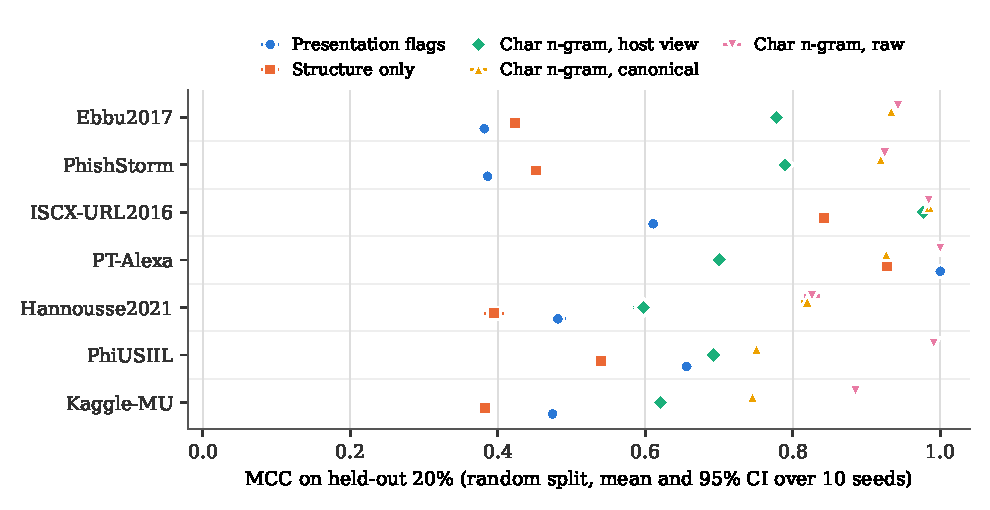
\includegraphics[width=\linewidth]{figures/fig_within.pdf}
\caption{Within-corpus MCC under a stratified random split (mean over 10 seeds; horizontal bars are 95\% CIs and are often narrower than the markers). Colour and marker shape both identify the detector. The lexical and presentation-plus-https detectors are omitted for legibility and appear in Table~\ref{tab:within_random}. The gap between the raw-string marker and the canonical marker measures dependence on presentation features; the gap between canonical and host-view markers measures dependence on path information, which includes the homepage-sampling artefact.}
\label{fig:within}
\end{figure}

\begin{table}[tp]
\centering
\caption{Within-corpus MCC (mean\,$\pm$\,95\% CI half-width over 10 repeated splits), stratified random 80/20 split. Pres.: the five presentation flags; Pres.+https adds the scheme-type flag.}
\label{tab:within_random}
\footnotesize
\setlength{\tabcolsep}{3pt}
\begin{adjustbox}{max width=\linewidth}
\begin{tabular}{@{}lrrrrrrr@{}}
\toprule
Corpus & Pres. & Pres.+https & Structure & Lexical & Char raw & Char canon. & Char host \\
\midrule
Ebbu2017 & 0.382\,$\pm$\,0.003 & 0.529\,$\pm$\,0.004 & 0.424\,$\pm$\,0.004 & 0.782\,$\pm$\,0.004 & 0.943\,$\pm$\,0.002 & 0.933\,$\pm$\,0.003 & 0.778\,$\pm$\,0.004 \\
PhishStorm & 0.386\,$\pm$\,0.004 & 0.386\,$\pm$\,0.003 & 0.452\,$\pm$\,0.008 & 0.752\,$\pm$\,0.003 & 0.925\,$\pm$\,0.002 & 0.919\,$\pm$\,0.002 & 0.789\,$\pm$\,0.004 \\
ISCX-URL2016 & 0.611\,$\pm$\,0.006 & 0.617\,$\pm$\,0.007 & 0.842\,$\pm$\,0.004 & 0.990\,$\pm$\,0.002 & 0.984\,$\pm$\,0.002 & 0.985\,$\pm$\,0.002 & 0.977\,$\pm$\,0.002 \\
PT-Alexa & 1.000\,$\pm$\,0.000 & 1.000\,$\pm$\,0.000 & 0.928\,$\pm$\,0.003 & 0.953\,$\pm$\,0.003 & 1.000\,$\pm$\,0.000 & 0.927\,$\pm$\,0.004 & 0.701\,$\pm$\,0.009 \\
Hannousse2021 & 0.482\,$\pm$\,0.010 & 0.482\,$\pm$\,0.010 & 0.395\,$\pm$\,0.013 & 0.738\,$\pm$\,0.006 & 0.826\,$\pm$\,0.011 & 0.820\,$\pm$\,0.008 & 0.598\,$\pm$\,0.014 \\
PhiUSIIL & 0.656\,$\pm$\,0.003 & 0.985\,$\pm$\,0.001 & 0.540\,$\pm$\,0.007 & 0.701\,$\pm$\,0.004 & 0.991\,$\pm$\,0.001 & 0.751\,$\pm$\,0.004 & 0.693\,$\pm$\,0.005 \\
Kaggle-MU & 0.474\,$\pm$\,0.004 & 0.513\,$\pm$\,0.005 & 0.383\,$\pm$\,0.007 & 0.564\,$\pm$\,0.008 & 0.885\,$\pm$\,0.002 & 0.745\,$\pm$\,0.004 & 0.621\,$\pm$\,0.007 \\
\bottomrule
\end{tabular}
\end{adjustbox}
\end{table}

\begin{table}[tp]
\centering
\caption{Presentation-probe ablation (MCC, random split, mean over 10 seeds). $-$X: probe without flag X (scheme: explicit scheme; slash: string ends in a slash; case: upper-case letter in the host). Path subset: probe trained and tested only on URLs that have a path, which removes the homepage-sampling contrast; --: fewer than 500 such URLs in one class. Last column: legitimate/phishing URLs with a path.}
\label{tab:probe}
\footnotesize
\setlength{\tabcolsep}{3pt}
\begin{adjustbox}{max width=\linewidth}
\begin{tabular}{@{}lrrrrrrrrr@{}}
\toprule
Corpus & All five & +https & $-$scheme & $-$www. & $-$slash & $-$\texttt{\&amp;} & $-$case & Path subset & $n$ with path (L/P) \\
\midrule
Ebbu2017 & 0.382 & 0.529 & 0.382 & 0.212 & 0.382 & 0.359 & 0.381 & 0.379 & 23,779/21,306 \\
PhishStorm & 0.386 & 0.386 & 0.386 & 0.228 & 0.386 & 0.359 & 0.386 & 0.383 & 24,920/24,941 \\
ISCX-URL2016 & 0.611 & 0.617 & 0.611 & 0.251 & 0.611 & 0.579 & 0.611 & 0.619 & 24,914/9,366 \\
PT-Alexa & 1.000 & 1.000 & 0.529 & 1.000 & 1.000 & 1.000 & 1.000 & -- & 0/11,024 \\
Hannousse2021 & 0.482 & 0.482 & 0.482 & 0.164 & 0.482 & 0.471 & 0.482 & 0.426 & 3,501/4,279 \\
PhiUSIIL & 0.656 & 0.985 & 0.656 & 0.475 & 0.640 & 0.654 & 0.656 & -- & 0/6,743 \\
Kaggle-MU & 0.474 & 0.513 & 0.454 & 0.176 & 0.474 & 0.474 & 0.474 & 0.609 & 21,949/18,349 \\
\bottomrule
\end{tabular}
\end{adjustbox}
\end{table}


\subsection{Removing presentation features}
\label{sec:canon}
Canonicalisation lowers the character model substantially on three corpora (Table~\ref{tab:tests}). On PhiUSIIL the MCC falls from \WPhiUSIILRandomCharRaw{} to \WPhiUSIILRandomCharCanon, a paired drop of \DRawVsCanonPhiUSIIL{} (ROC-AUC drop \DARawVsCanonPhiUSIIL); on Kaggle-MU it falls by \DRawVsCanonKaggleMU{} and on PT-Alexa by \DRawVsCanonPTAlexa. On the four other corpora the mean drop is below 0.01. Its corrected 95\% interval is widest on Hannousse2021 (\DLoRawVsCanonHannousse{} to \DHiRawVsCanonHannousse), so these data cannot exclude a formatting dependence of a few hundredths there, but they exclude one of the size seen on PhiUSIIL and Kaggle-MU. These four corpora have moderate presentation probes, yet their character models do not rely on the formatting flags.

Further controls test competing explanations (Tables~\ref{tab:controls} and~\ref{tab:controls2}). Kaggle-MU's drop could reflect its label inconsistencies rather than formatting, because many of its contested rows are scheme-less. On Kaggle-MU-clean, which removes the \KCleanNMixedRows{} rows of registered domains with both labels and the phishing rows that another corpus labels legitimate, the raw-string model reaches \KCleanCharRaw{} and the canonical model \KCleanCharCanon. That rule misses a second group of doubtful rows: \KCleanBareWwwPct\% of the remaining phishing class starts with a bare \texttt{www.}, mostly content pages of small software, publishing and research sites (largest registered domains \KWwwTopDomains), and only \KWwwKwShare\% of these rows contain a brand or credential keyword, against \KOtherKwShare\% of the other phishing rows. They look like a list of benign pages that received the phishing label. Without them the probe falls to \KCleanTwoPresentationHttps, while the raw-string model reaches \KCleanTwoCharRaw{} and the canonical model \KCleanTwoCharCanon, a drop of \KCleanTwoDrop. Kaggle-MU's character model therefore depends on formatting beyond these rows, but in a collection that mixes sources this way we cannot say how much of the dependence is a phishing feed's convention and how much marks the source a row came from. Among Kaggle-MU homepages the contrast is extreme: the probe reaches \HomeKaggleMUPresentationHttps, the raw-string model \HomeKaggleMUCharRaw{} and the canonical model \HomeKaggleMUCharCanon, because \HomeSlashLegitKaggleMU\% of legitimate homepage strings end in a slash against \HomeSlashPhishKaggleMU\% of phishing ones.

Adding a single token for an explicit \texttt{https} scheme to the canonical string raises PhiUSIIL from \WPhiUSIILRandomCharCanon{} to \CanonHttpsPhiUSIIL, so most of its formatting dependence is carried by the scheme type. This is not evidence of a server property: every legitimate PhiUSIIL string carries the same \texttt{https://www.} prefix, a curator's template. On the other corpora the token changes the canonical model by between \CanonHttpsGainPhishStorm{} and \CanonHttpsGainPTAlexa{} MCC. In the PhishTank dump, where submission times allow a time split, training on phishing URLs submitted up to 2019 (\TimeTrainHttps\% with \texttt{https}) and testing on 2020 submissions (\TimeTestHttps\%) gives the canonical model \TimeCharCanon{} against \TimeRandCharCanon{} for a split of the same size drawn from all years, and \TimeCharCanonHttps{} against \TimeRandCharCanonHttps{} with the scheme token, a loss of \TimeGapCharCanon{} and \TimeGapCharCanonHttps{} MCC when the phishing class of the test set is newer than that of the training set and the legitimate class is held fixed. The raw-string model and the probe stay at \TimeCharRaw{} and \TimePresentationHttps{}, because the scheme convention that separates PT-Alexa does not change over time.

Table~\ref{tab:precision} converts the test error rates into the precision a detector would reach at 1\% and 0.1\% phishing prevalence. At the default threshold of 0.5 the canonical model stays at or below \PrecOneEbbuRandomCharCanon{} at 1\% prevalence on every published corpus except ISCX-URL2016 (\PrecOneISCXURLRandomCharCanon{} random, \PrecOneISCXURLDomainCharCanon{} grouped). The raw-string model on PhiUSIIL is the exception that formatting allows: it made no false positive in any of the 10 seeds, each with \NLegTestPhiUSIIL{} legitimate test URLs, so a conservative per-seed 95\% upper bound on its false-positive rate is about 3 in \NLegTestPhiUSIIL. A threshold chosen on validation data for a false-positive rate of at most 0.1\% keeps that rate on the test part of the same corpus: the realised rate of the canonical model lies between \VFprHannousseCharCanon\% (Hannousse2021) and \VFprEbbuCharCanon\% (Ebbu2017). At 1\% prevalence this gives the canonical model a precision of \VPrecOneEbbuCharCanon{} on Ebbu2017, \VPrecOnePhishStormCharCanon{} on PhishStorm and \VPrecOneKaggleMUCharCanon{} on Kaggle-MU, at true-positive rates of \VTprEbbuCharCanon, \VTprPhishStormCharCanon{} and \VTprKaggleMUCharCanon. At 0.1\% prevalence no published corpus gives the canonical model a precision above \VPrecTenthISCXURLCharCanon, so most alarms would still be false. The low rate is reached at a cost in recall that the balanced MCC hides; on Hannousse2021 the true-positive rate falls to \VTprHannousseCharCanon, and its \VNZeroHannousseCharCanon{} legitimate test URLs over ten seeds yield only \VFPHannousseCharCanon{} false positives, so its rates are imprecise.

\begin{table}[tp]
\centering
\caption{Test-set error rates and the precision a within-corpus detector would reach at 1\% and 0.1\% phishing prevalence (random split, 10 seeds). Validation threshold: 20\% of the training part is held out, the model is fitted on the rest, and the threshold with the highest validation true-positive rate at a validation false-positive rate of at most 0.1\% is applied to the test part; FPR and TPR are the realised test rates. @0.5: the model fitted on the full training part at threshold 0.5. Rates are pooled over seeds before precision is computed.}
\label{tab:precision}
\footnotesize
\setlength{\tabcolsep}{3pt}
\begin{adjustbox}{max width=\linewidth}
\begin{tabular}{@{}lrrrrrrrrrr@{}}
\toprule
 & \multicolumn{5}{c}{Char raw} & \multicolumn{5}{c}{Char canon.} \\
\cmidrule(lr){2-6}\cmidrule(lr){7-11}
 & \multicolumn{4}{c}{Validation threshold} & @0.5 & \multicolumn{4}{c}{Validation threshold} & @0.5 \\
\cmidrule(lr){2-5}\cmidrule(lr){6-6}\cmidrule(lr){7-10}\cmidrule(lr){11-11}
Corpus & FPR (\%) & TPR & Prec.\ 1\% & Prec.\ 0.1\% & Prec.\ 1\% & FPR (\%) & TPR & Prec.\ 1\% & Prec.\ 0.1\% & Prec.\ 1\% \\
\midrule
Ebbu2017 & 0.14 & 0.766 & 0.850 & 0.360 & 0.277 & 0.16 & 0.730 & 0.820 & 0.311 & 0.293 \\
PhishStorm & 0.12 & 0.753 & 0.862 & 0.382 & 0.279 & 0.11 & 0.712 & 0.869 & 0.398 & 0.265 \\
ISCX-URL2016 & 0.10 & 0.974 & 0.908 & 0.494 & 0.906 & 0.11 & 0.947 & 0.900 & 0.472 & 0.847 \\
PT-Alexa & 0.00 & 1.000 & 1.000 & 1.000 & 1.000 & 0.11 & 0.779 & 0.879 & 0.420 & 0.611 \\
Hannousse2021 & 0.07 & 0.343 & 0.832 & 0.329 & 0.101 & 0.05 & 0.206 & 0.798 & 0.282 & 0.128 \\
PhiUSIIL & 0.10 & 0.995 & 0.913 & 0.509 & 1.000 & 0.13 & 0.585 & 0.820 & 0.311 & 0.128 \\
Kaggle-MU & 0.15 & 0.199 & 0.570 & 0.116 & 0.153 & 0.11 & 0.127 & 0.548 & 0.107 & 0.055 \\
\bottomrule
\end{tabular}
\end{adjustbox}
\end{table}

\begin{table}[tp]
\centering
\caption{Controls (MCC, random split, mean over 10 seeds). Homepage subset: only URLs without a path, so that both classes are sampled at the same granularity; $n$: legitimate and phishing homepages in the capped sample; --: fewer than 500 such URLs in one class. Full corpus: the canonical model of Table~\ref{tab:within_random} and the same model with a token for an explicit \texttt{https} scheme prepended to the canonical string.}
\label{tab:controls}
\footnotesize
\begin{adjustbox}{max width=\linewidth}
\begin{tabular}{@{}lrrrrrr@{}}
\toprule
 & \multicolumn{4}{c}{Homepage subset (no path in either class)} & \multicolumn{2}{c}{Full corpus} \\
\cmidrule(lr){2-5}\cmidrule(lr){6-7}
Corpus & $n$ (L/P) & Pres.+https & Char raw & Char canon. & Char canon. & Canon.+https \\
\midrule
Ebbu2017 & 1,248/509 & 0.464 & 0.779 & 0.721 & 0.933 & 0.942 \\
PhishStorm & 90/60 & -- & -- & -- & 0.919 & 0.919 \\
ISCX-URL2016 & 81/370 & -- & -- & -- & 0.985 & 0.987 \\
PT-Alexa & 15,753/2,193 & 1.000 & 0.999 & 0.698 & 0.927 & 0.947 \\
Hannousse2021 & 2,213/1,077 & 0.556 & 0.783 & 0.708 & 0.820 & 0.828 \\
PhiUSIIL & 25,000/18,433 & 0.996 & 0.991 & 0.709 & 0.751 & 0.967 \\
Kaggle-MU & 3,033/6,607 & 0.933 & 0.925 & 0.503 & 0.745 & 0.751 \\
\bottomrule
\end{tabular}
\end{adjustbox}
\end{table}

\begin{table}[tp]
\centering
\caption{Kaggle-MU subsets and a time split (MCC, mean over seeds). Kaggle-MU rows: random split, 10 seeds, at most 25,000 URLs per class; $n$: legitimate/phishing rows before the cap. Kaggle-MU-clean drops registered domains with both labels and phishing URLs that another corpus labels legitimate; the next row also drops phishing URLs that start with a bare \texttt{www.} (the rule also removes phishing URLs on Alexa top-1,000 domains, but none remain after the first rule). PT-Alexa rows: 3 seeds; $n$: phishing URLs for training/testing, with as many legitimate URLs drawn at random; the time split trains on phishing URLs submitted up to 2019 and tests on 2020 submissions, the matched control draws the same numbers from all years.}
\label{tab:controls2}
\footnotesize
\setlength{\tabcolsep}{3pt}
\begin{adjustbox}{max width=\linewidth}
\begin{tabular}{@{}>{\raggedright\arraybackslash}p{4.2cm}rrrrr@{}}
\toprule
Control & $n$ & Pres.+https & Char raw & Char canon. & Canon.+https \\
\midrule
Kaggle-MU, full & 509,092 in all & 0.513 & 0.885 & 0.745 & -- \\
Kaggle-MU-clean & 312,932/52,034 & 0.474 & 0.904 & 0.739 & -- \\
Kaggle-MU-clean without bare-\texttt{www.} phishing & 312,932/37,968 & 0.351 & 0.904 & 0.763 & -- \\
\midrule
PT-Alexa, random years (matched) & 2,373/5,000 & 1.000 & 1.000 & 0.898 & 0.924 \\
PT-Alexa, train $\le$2019, test 2020 & 2,373/5,000 & 1.000 & 1.000 & 0.865 & 0.897 \\
\bottomrule
\end{tabular}
\end{adjustbox}
\end{table}


\begin{table}[tp]
\centering
\caption{Differences paired by seed over 10 repeated splits: mean MCC and ROC-AUC difference with a 95\% interval that uses the variance correction of \citet{nadeau2003}, and a Holm-adjusted $p$-value from the corrected resampled $t$-test across the seven corpora of each comparison. For the random-versus-grouped comparisons the two settings share the sample of a seed but not the split. Differences smaller than 0.0005 in absolute value print as $+$0.000; small $p$-values for such rows reflect very small seed variance, not a material effect.}
\label{tab:tests}
\footnotesize
\scriptsize
\setlength{\tabcolsep}{3pt}
\begin{adjustbox}{max width=\linewidth}
\begin{tabular}{@{}lrrrr@{}}
\toprule
Comparison and corpus & $\Delta$MCC [95\% CI] & $p_\mathrm{Holm}$ & $\Delta$AUC [95\% CI] & $p_\mathrm{Holm}$ \\
\midrule
\multicolumn{5}{@{}l}{\emph{Char raw $-$ canonical (random split)}} \\
\quad Ebbu2017 & +0.009 [+0.004, +0.014] & 0.012 & +0.001 [+0.001, +0.002] & 0.006 \\
\quad PhishStorm & +0.006 [+0.002, +0.009] & 0.017 & +0.001 [+0.000, +0.001] & 0.008 \\
\quad ISCX-URL2016 & $-$0.001 [$-$0.005, +0.003] & 1.000 & +0.000 [+0.000, +0.000] & 0.008 \\
\quad PT-Alexa & +0.073 [+0.066, +0.080] & $<$0.001 & +0.010 [+0.008, +0.012] & $<$0.001 \\
\quad Hannousse2021 & +0.006 [$-$0.014, +0.027] & 1.000 & +0.005 [+0.001, +0.010] & 0.028 \\
\quad PhiUSIIL & +0.240 [+0.234, +0.246] & $<$0.001 & +0.070 [+0.066, +0.073] & $<$0.001 \\
\quad Kaggle-MU & +0.140 [+0.133, +0.147] & $<$0.001 & +0.038 [+0.037, +0.039] & $<$0.001 \\
\multicolumn{5}{@{}l}{\emph{Char raw $-$ host view (random split)}} \\
\quad Ebbu2017 & +0.165 [+0.156, +0.173] & $<$0.001 & +0.040 [+0.037, +0.042] & $<$0.001 \\
\quad PhishStorm & +0.136 [+0.129, +0.143] & $<$0.001 & +0.033 [+0.031, +0.035] & $<$0.001 \\
\quad ISCX-URL2016 & +0.007 [+0.003, +0.012] & 0.003 & +0.000 [+0.000, +0.001] & 0.016 \\
\quad PT-Alexa & +0.299 [+0.282, +0.317] & $<$0.001 & +0.078 [+0.072, +0.085] & $<$0.001 \\
\quad Hannousse2021 & +0.228 [+0.208, +0.248] & $<$0.001 & +0.086 [+0.077, +0.095] & $<$0.001 \\
\quad PhiUSIIL & +0.298 [+0.290, +0.307] & $<$0.001 & +0.089 [+0.085, +0.094] & $<$0.001 \\
\quad Kaggle-MU & +0.264 [+0.252, +0.277] & $<$0.001 & +0.084 [+0.081, +0.087] & $<$0.001 \\
\multicolumn{5}{@{}l}{\emph{Random $-$ grouped split, char canonical}} \\
\quad Ebbu2017 & +0.025 [+0.017, +0.033] & $<$0.001 & +0.003 [+0.001, +0.005] & 0.020 \\
\quad PhishStorm & +0.037 [+0.023, +0.050] & 0.001 & +0.007 [+0.003, +0.010] & 0.017 \\
\quad ISCX-URL2016 & +0.030 [+0.018, +0.042] & 0.002 & +0.002 [+0.001, +0.002] & 0.004 \\
\quad PT-Alexa & +0.011 [+0.001, +0.022] & 0.118 & +0.001 [$-$0.002, +0.004] & 0.798 \\
\quad Hannousse2021 & +0.006 [$-$0.014, +0.026] & 1.000 & +0.005 [+0.001, +0.008] & 0.059 \\
\quad PhiUSIIL & +0.003 [$-$0.008, +0.014] & 1.000 & +0.001 [$-$0.003, +0.005] & 0.798 \\
\quad Kaggle-MU & +0.077 [+0.042, +0.111] & 0.003 & +0.027 [+0.012, +0.042] & 0.017 \\
\multicolumn{5}{@{}l}{\emph{Random $-$ grouped split, lexical}} \\
\quad Ebbu2017 & +0.025 [+0.004, +0.045] & 0.132 & +0.008 [+0.000, +0.016] & 0.261 \\
\quad PhishStorm & +0.037 [$-$0.003, +0.077] & 0.267 & +0.013 [+0.000, +0.025] & 0.261 \\
\quad ISCX-URL2016 & +0.071 [+0.006, +0.136] & 0.182 & +0.005 [+0.000, +0.009] & 0.261 \\
\quad PT-Alexa & $-$0.001 [$-$0.009, +0.007] & 1.000 & $-$0.000 [$-$0.002, +0.001] & 1.000 \\
\quad Hannousse2021 & +0.015 [$-$0.006, +0.037] & 0.420 & +0.002 [$-$0.005, +0.009] & 1.000 \\
\quad PhiUSIIL & $-$0.001 [$-$0.007, +0.005] & 1.000 & +0.001 [$-$0.004, +0.006] & 1.000 \\
\quad Kaggle-MU & +0.082 [+0.035, +0.129] & 0.023 & +0.061 [+0.036, +0.085] & 0.002 \\
\multicolumn{5}{@{}l}{\emph{Random $-$ grouped split, char host view}} \\
\quad Ebbu2017 & +0.222 [+0.201, +0.243] & $<$0.001 & +0.078 [+0.063, +0.093] & $<$0.001 \\
\quad PhishStorm & +0.193 [+0.116, +0.271] & $<$0.001 & +0.077 [+0.035, +0.119] & 0.005 \\
\quad ISCX-URL2016 & +0.727 [+0.656, +0.798] & $<$0.001 & +0.208 [+0.144, +0.273] & $<$0.001 \\
\quad PT-Alexa & +0.298 [+0.266, +0.330] & $<$0.001 & +0.222 [+0.208, +0.236] & $<$0.001 \\
\quad Hannousse2021 & +0.051 [+0.018, +0.083] & 0.012 & +0.037 [+0.018, +0.055] & 0.004 \\
\quad PhiUSIIL & +0.012 [$-$0.001, +0.026] & 0.072 & +0.005 [+0.000, +0.010] & 0.033 \\
\quad Kaggle-MU & +0.189 [+0.146, +0.232] & $<$0.001 & +0.104 [+0.071, +0.137] & $<$0.001 \\
\bottomrule
\end{tabular}
\end{adjustbox}
\end{table}


\subsection{Host view and registered-domain grouping}
\label{sec:domain}
The host view removes the path as well. Under the random split it costs the character model between \DRawVsHostISCXURL{} (ISCX-URL2016) and \DRawVsHostPTAlexa{} (PT-Alexa) MCC. Part of that information is genuine, since phishing kits sit in deep paths; part is the sampling artefact of homepage-only legitimate sets. The grouped split separates the two for one corpus. On ISCX-URL2016 the host-view model reaches \WISCXURLRandomCharHost{} under the random split and \WISCXURLDomainCharHost{} under the grouped split, because a random split lets it memorise the \RegLegitISCXURL{} legitimate registered domains.

Grouping by registered domain gives a lower mean MCC for the canonical character model on every corpus, by between \DCanonRandomVsDomainPhiUSIIL{} (PhiUSIIL) and \DCanonRandomVsDomainKaggleMU{} (Kaggle-MU); the difference survives Holm adjustment on four corpora (Ebbu2017, PhishStorm, ISCX-URL2016 and Kaggle-MU). The two splits of a seed share the sample but not the partition, so these comparisons are paired by seed only. The lexical model changes significantly only on Kaggle-MU. Domain leakage thus inflates the full-URL n-gram and lexical models by up to \DLexicalRandomVsDomainKaggleMU{} MCC (lexical model on Kaggle-MU) and host-only models by much more: the host-view drop ranges from \DHostRandomVsDomainPhiUSIIL{} to \DHostRandomVsDomainISCXURL. The stratified group partition keeps the test share and the class prior of the grouped split equal to those of the random split to within 0.01 on every corpus, so these differences are not caused by a change of prior. A detector that sees no domain information serves as a check: on PhiUSIIL the presentation probe gives \WPhiUSIILRandomPresentation{} under the random and \WPhiUSIILDomainPresentation{} under the grouped split. Table~\ref{tab:within_domain} gives all grouped-split results.

\begin{table}[tp]
\centering
\caption{Within-corpus MCC (mean\,$\pm$\,95\% CI half-width over 10 repeated splits), stratified 80/20 split with disjoint registered domains (first fold of a shuffled stratified group 5-fold partition). Pres.: the five presentation flags; Pres.+https adds the scheme-type flag.}
\label{tab:within_domain}
\footnotesize
\setlength{\tabcolsep}{3pt}
\begin{adjustbox}{max width=\linewidth}
\begin{tabular}{@{}lrrrrrrr@{}}
\toprule
Corpus & Pres. & Pres.+https & Structure & Lexical & Char raw & Char canon. & Char host \\
\midrule
Ebbu2017 & 0.294\,$\pm$\,0.049 & 0.546\,$\pm$\,0.019 & 0.410\,$\pm$\,0.020 & 0.757\,$\pm$\,0.011 & 0.924\,$\pm$\,0.004 & 0.908\,$\pm$\,0.006 & 0.556\,$\pm$\,0.013 \\
PhishStorm & 0.287\,$\pm$\,0.043 & 0.280\,$\pm$\,0.044 & 0.413\,$\pm$\,0.018 & 0.715\,$\pm$\,0.019 & 0.894\,$\pm$\,0.006 & 0.883\,$\pm$\,0.007 & 0.596\,$\pm$\,0.042 \\
ISCX-URL2016 & 0.599\,$\pm$\,0.070 & 0.599\,$\pm$\,0.069 & 0.786\,$\pm$\,0.042 & 0.919\,$\pm$\,0.035 & 0.962\,$\pm$\,0.008 & 0.955\,$\pm$\,0.007 & 0.250\,$\pm$\,0.039 \\
PT-Alexa & 1.000\,$\pm$\,0.000 & 1.000\,$\pm$\,0.000 & 0.927\,$\pm$\,0.003 & 0.954\,$\pm$\,0.002 & 1.000\,$\pm$\,0.000 & 0.916\,$\pm$\,0.004 & 0.403\,$\pm$\,0.010 \\
Hannousse2021 & 0.454\,$\pm$\,0.015 & 0.454\,$\pm$\,0.015 & 0.368\,$\pm$\,0.039 & 0.722\,$\pm$\,0.011 & 0.816\,$\pm$\,0.009 & 0.814\,$\pm$\,0.008 & 0.547\,$\pm$\,0.011 \\
PhiUSIIL & 0.674\,$\pm$\,0.011 & 0.984\,$\pm$\,0.002 & 0.564\,$\pm$\,0.013 & 0.702\,$\pm$\,0.004 & 0.990\,$\pm$\,0.001 & 0.748\,$\pm$\,0.006 & 0.680\,$\pm$\,0.007 \\
Kaggle-MU & 0.413\,$\pm$\,0.025 & 0.464\,$\pm$\,0.019 & 0.353\,$\pm$\,0.017 & 0.482\,$\pm$\,0.022 & 0.850\,$\pm$\,0.026 & 0.669\,$\pm$\,0.017 & 0.432\,$\pm$\,0.023 \\
\bottomrule
\end{tabular}
\end{adjustbox}
\end{table}


\subsection{A neural character model}
\label{sec:cnn}
The character CNN separates the corpora in the same way as the n-gram model (Table~\ref{tab:cnn}). Canonicalisation costs it \CNNDropPhiUSIILRandom{} MCC on PhiUSIIL, \CNNDropKaggleMURandom{} on Kaggle-MU and \CNNDropPTAlexaRandom{} on PT-Alexa under the random split, and between \CNNDropISCXURLRandom{} and \CNNDropHannousseRandom{} on the four other corpora. On PhiUSIIL the raw CNN reaches \CNNPhiUSIILRandomRaw{} and the canonical CNN \CNNPhiUSIILRandomCanon{}, close to the values of the logistic model; the CNN as trained here finds no more phishing evidence in the canonical strings than the n-gram model. The CNN depends on formatting more than the n-gram model on the four other corpora: its drop is \CNNDropEbbuRandom{} on Ebbu2017 against \DRawVsCanonEbbu{} for the n-gram model, and under the grouped split it reaches \CNNDropISCXURLDomain{} on ISCX-URL2016 and \CNNDropPhishStormDomain{} on PhishStorm. The CNN is trained for a fixed five epochs without a validation set and with three seeds, and on ISCX-URL2016 under the grouped split its canonical MCC ranges from \CNNMinISCXURLDomainCanon{} to \CNNMaxISCXURLDomainCanon{} across seeds. We therefore read it as a check on the direction of the effect, not as a competitor, and do not test its differences.

\begin{table}[tp]
\centering
\caption{Character-level CNN (URLNet character branch) against the character n-gram logistic regression (LR): MCC, mean (standard deviation) over seeds 0--2 for the CNN and mean over seeds 0--9 for LR, same caps and split procedure. The CNN is trained for a fixed five epochs without a validation set.}
\label{tab:cnn}
\footnotesize
\begin{adjustbox}{max width=\linewidth}
\begin{tabular}{@{}lrrrrrr@{}}
\toprule
 & \multicolumn{3}{c}{Random split} & \multicolumn{3}{c}{Grouped split} \\
\cmidrule(lr){2-4}\cmidrule(lr){5-7}
Corpus & CNN raw & CNN canon. & LR raw / canon. & CNN raw & CNN canon. & LR raw / canon. \\
\midrule
Ebbu2017 & 0.923 (0.006) & 0.901 (0.005) & 0.943 / 0.933 & 0.907 (0.015) & 0.879 (0.020) & 0.924 / 0.908 \\
PhishStorm & 0.901 (0.006) & 0.885 (0.004) & 0.925 / 0.919 & 0.862 (0.034) & 0.832 (0.045) & 0.894 / 0.883 \\
ISCX-URL2016 & 0.987 (0.001) & 0.983 (0.003) & 0.984 / 0.985 & 0.934 (0.050) & 0.885 (0.108) & 0.962 / 0.955 \\
PT-Alexa & 1.000 (0.000) & 0.948 (0.006) & 1.000 / 0.927 & 1.000 (0.000) & 0.946 (0.005) & 1.000 / 0.916 \\
Hannousse2021 & 0.777 (0.017) & 0.751 (0.009) & 0.826 / 0.820 & 0.766 (0.020) & 0.749 (0.027) & 0.816 / 0.814 \\
PhiUSIIL & 0.997 (0.001) & 0.751 (0.003) & 0.991 / 0.751 & 0.997 (0.001) & 0.753 (0.007) & 0.990 / 0.748 \\
Kaggle-MU & 0.893 (0.004) & 0.679 (0.005) & 0.885 / 0.745 & 0.833 (0.022) & 0.607 (0.025) & 0.850 / 0.669 \\
\bottomrule
\end{tabular}
\end{adjustbox}
\end{table}


\subsection{Transfer across corpora}
\label{sec:cross}
Figure~\ref{fig:cross} and Table~\ref{tab:pair_url} report transfer between corpora after the URL purge. The presentation probe transfers at chance on average (mean ROC-AUC \XUrlPresentationMeanAUC) but not uniformly: its pair-level AUC ranges from \XUrlPresentationMinAUC{} to \XUrlPresentationMaxAUC. An AUC far below 0.5 means that the formatting property that marks legitimate URLs in the training corpus marks phishing URLs in the test corpus. The presentation signal is therefore a property of each collection, with a direction that changes from corpus to corpus.

Canonicalisation improves average transfer modestly. Averaged over the test corpora of each training corpus, the canonical character model has a higher ROC-AUC than the raw-string model by \XTUrlCharCanonMinusCharRawAucCorpus{} (95\% CI \XTUrlCharCanonMinusCharRawAucCorpusLo{} to \XTUrlCharCanonMinusCharRawAucCorpusHi; higher for \XTUrlCharCanonMinusCharRawAucCorpusBetter{} of 7 training corpora, Wilcoxon $p=\XTUrlCharCanonMinusCharRawAucP$) and a higher MCC by \XTUrlCharCanonMinusCharRawMccCorpus{} (\XTUrlCharCanonMinusCharRawMccCorpusBetter{} of 7, $p=\XTUrlCharCanonMinusCharRawMccP$). With seven units the attainable two-sided values are 0.016, 0.031, 0.047 and larger, so these are the third-smallest and the smallest, and the AUC interval touches zero; the AUC gain is consistent but modest. It is also concentrated. In the \XInvN{} pairs where the presentation probe has an AUC below 0.5, that is, where the formatting conventions of the two corpora point in opposite directions, canonicalisation raises AUC by \XInvGain{} on average; in the other \XOthN{} pairs by \XOthGain. Without Kaggle-MU, which we do not recommend as an independent benchmark, the corpus-level gain is \XNoKGain{} (95\% CI \XNoKLo{} to \XNoKHi; higher for \XNoKBetter{} of \XNoKN, $p=\XNoKP$). Canonical input therefore mainly prevents failures caused by inverted conventions; it does not make a detector generalise in general. Pair-level results are not independent, because each test corpus appears in six pairs. Averaging per test corpus instead gives a gain of \XByTestGain{} (higher for \XByTestBetter{} of \XByTestN, $p=\XByTestP$), and \XByTestNoKGain{} without Kaggle-MU (\XByTestNoKBetter{} of \XByTestNoKN, $p=\XByTestNoKP$); we do not model the two dependences jointly. The host view does not transfer better than the raw string (AUC difference \XTUrlCharHostMinusCharRawAucCorpus, $p=\XTUrlCharHostMinusCharRawAucP$). The canonical character model also beats the lexical feature model (AUC difference \XTUrlCharCanonMinusLexicalAucCorpus, $p=\XTUrlCharCanonMinusLexicalAucP$). The stricter domain purge leaves these conclusions unchanged (Table~\ref{tab:pair_domain}): the canonical model's mean AUC moves from \XUrlCharCanonMeanAUC{} to \XDomainCharCanonMeanAUC{} and the raw model's from \XUrlCharRawMeanAUC{} to \XDomainCharRawMeanAUC.

Artefacts can also inflate transfer. A raw-string model trained on Ebbu2017, whose legitimate URLs carry \texttt{https} far more often than its phishing URLs, ranks PhiUSIIL almost perfectly (AUC \XCUrlCharRawEbbuPhiUSIIL); after canonicalisation the same pair falls to \XCUrlCharCanonEbbuPhiUSIIL. A single transfer result therefore cannot certify that a detector learned phishing, since the training and test corpora may share a formatting convention by chance. The reverse also occurs: raw-string models trained on Kaggle-MU and on PT-Alexa rank PhiUSIIL below chance (AUC \XCUrlCharRawKaggleMUPhiUSIIL{} and \XCUrlCharRawPTAlexaPhiUSIIL), consistent with formatting conventions that point the other way in PhiUSIIL. Ordering the pairs by the publication year of each corpus gives a coarse view of time, with two caveats: publication year is a proxy, since Kaggle-MU (2021) reuses older collections, and the \XTimeSameNPairs{} pairs between corpora of the same year are left out. PT-Alexa is placed in 2020, the last year of its PhishTank dump, and Ebbu2017 in 2019, the year of its paper. The canonical model reaches a mean AUC of \XTimeForwardCharCanon{} when it is trained on an older corpus and tested on a newer one (\XTimeForwardNPairs{} pairs) and \XTimeBackwardCharCanon{} in the other direction (\XTimeBackwardNPairs{} pairs), against \XTimeForwardCharRaw{} and \XTimeBackwardCharRaw{} for raw strings, so the canonical advantage holds in both directions. A threshold chosen on validation data from the training corpus does not keep its false-positive rate on another corpus. Set for a validation false-positive rate of at most 0.1\%, the canonical model has a median realised rate of \XVFprCharCanon\% over the \XVNPairsCharCanon{} pairs, more than ten times the target in \XVOverTenCharCanon{} of them, which gives a median precision of \XVPrecOneCharCanon{} at 1\% prevalence and \XVPrecTenthCharCanon{} at 0.1\%; the raw-string model has a median rate of \XVFprCharRaw\%. Set for 1\%, the canonical model's median realised rate is \XVFprOnePctCharCanon\%, and at threshold 0.5 it is \XVFprHalfCharCanon{} (precision \XVPrecOneHalfCharCanon{} at 1\%).

\begin{figure}[t]
\centering
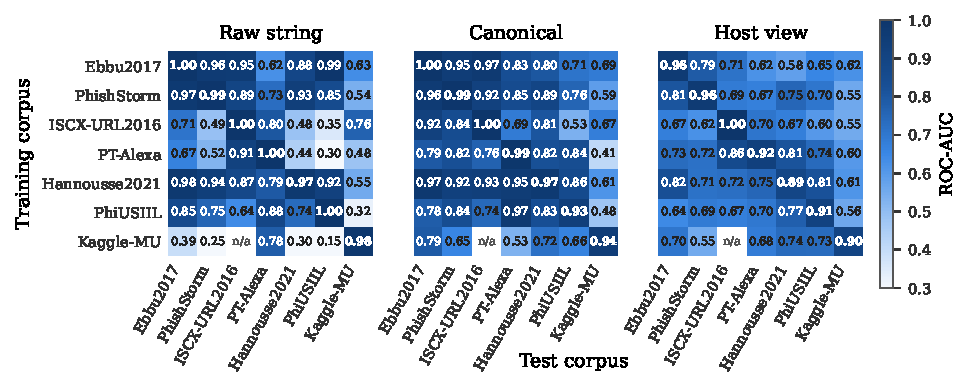
\includegraphics[width=\linewidth]{figures/fig_cross.pdf}
\caption{ROC-AUC of character n-gram models trained on one corpus (rows) and tested on another (columns), for raw strings, canonical strings and the host view. Off-diagonal cells average three seeds after removing test URLs whose canonical form occurs anywhere in the training corpus; diagonal cells (bold) are within-corpus random-split results averaged over ten seeds, without purging, and are shown for reference only. The cell marked n/a has no legitimate test URL left after purging. Darker cells are higher; the colour scale runs from 0.3 to 1.0 and values below 0.3 take the lightest colour.}
\label{fig:cross}
\end{figure}

\begin{table}[tp]
\centering
\caption{Cross-corpus transfer: ROC-AUC (MCC at threshold 0.5) averaged over the test corpora of each training corpus (five for Kaggle-MU, whose ISCX-URL2016 test set is empty after purging), and over all ordered pairs that keep both classes after purging; three seeds. Purging changes the size and class prior of a test set, which affects MCC but not ROC-AUC; per-pair sizes and priors are stored with the results. Test URLs whose canonical form occurs anywhere in the full training corpus are removed.}
\label{tab:pair_url}
\footnotesize
\begin{adjustbox}{max width=\linewidth}
\begin{tabular}{@{}lrrrrrr@{}}
\toprule
Training corpus & Pres. & Pres.+https & Lexical & Char raw & Char canon. & Char host \\
\midrule
Ebbu2017 & 0.519 (0.122) & 0.548 (-0.035) & 0.828 (0.490) & 0.840 (0.425) & 0.823 (0.487) & 0.661 (0.240) \\
PhishStorm & 0.554 (0.063) & 0.572 (0.063) & 0.771 (0.339) & 0.818 (0.481) & 0.826 (0.517) & 0.695 (0.279) \\
ISCX-URL2016 & 0.302 (-0.446) & 0.444 (-0.224) & 0.573 (-0.002) & 0.598 (0.173) & 0.744 (0.289) & 0.637 (0.153) \\
PT-Alexa & 0.506 (0.007) & 0.506 (0.007) & 0.581 (0.156) & 0.554 (0.016) & 0.741 (0.203) & 0.742 (0.346) \\
Hannousse2021 & 0.543 (0.042) & 0.589 (0.042) & 0.855 (0.567) & 0.841 (0.454) & 0.875 (0.606) & 0.739 (0.318) \\
PhiUSIIL & 0.544 (0.009) & 0.542 (0.059) & 0.623 (0.198) & 0.698 (0.083) & 0.771 (0.261) & 0.671 (0.243) \\
Kaggle-MU & 0.462 (0.191) & 0.527 (-0.024) & 0.630 (0.099) & 0.372 (0.009) & 0.670 (0.248) & 0.680 (0.253) \\
\midrule
All 41 pairs & 0.491 (-0.007) & 0.533 (-0.016) & 0.696 (0.268) & 0.682 (0.240) & 0.781 (0.376) & 0.690 (0.262) \\
\bottomrule
\end{tabular}
\end{adjustbox}
\end{table}

\begin{table}[tp]
\centering
\caption{Cross-corpus transfer: ROC-AUC (MCC at threshold 0.5) averaged over the test corpora of each training corpus (five for Kaggle-MU, whose ISCX-URL2016 test set is empty after purging), and over all ordered pairs that keep both classes after purging; three seeds. Purging changes the size and class prior of a test set, which affects MCC but not ROC-AUC; per-pair sizes and priors are stored with the results. Test URLs whose canonical form or registered domain occurs anywhere in the full training corpus are removed.}
\label{tab:pair_domain}
\footnotesize
\begin{adjustbox}{max width=\linewidth}
\begin{tabular}{@{}lrrrrrr@{}}
\toprule
Training corpus & Pres. & Pres.+https & Lexical & Char raw & Char canon. & Char host \\
\midrule
Ebbu2017 & 0.522 (0.130) & 0.551 (-0.027) & 0.822 (0.472) & 0.837 (0.413) & 0.815 (0.462) & 0.623 (0.185) \\
PhishStorm & 0.562 (0.073) & 0.577 (0.073) & 0.782 (0.350) & 0.831 (0.483) & 0.838 (0.522) & 0.679 (0.242) \\
ISCX-URL2016 & 0.300 (-0.452) & 0.444 (-0.229) & 0.575 (-0.002) & 0.595 (0.168) & 0.743 (0.285) & 0.630 (0.138) \\
PT-Alexa & 0.511 (0.024) & 0.511 (0.024) & 0.605 (0.187) & 0.533 (0.031) & 0.736 (0.214) & 0.689 (0.242) \\
Hannousse2021 & 0.546 (0.046) & 0.586 (0.046) & 0.841 (0.542) & 0.823 (0.429) & 0.864 (0.580) & 0.691 (0.253) \\
PhiUSIIL & 0.531 (-0.020) & 0.544 (0.041) & 0.636 (0.207) & 0.691 (0.080) & 0.769 (0.271) & 0.648 (0.210) \\
Kaggle-MU & 0.435 (0.192) & 0.512 (-0.038) & 0.592 (0.054) & 0.347 (-0.013) & 0.640 (0.190) & 0.638 (0.175) \\
\midrule
All 41 pairs & 0.488 (-0.006) & 0.533 (-0.015) & 0.696 (0.264) & 0.673 (0.233) & 0.775 (0.365) & 0.657 (0.207) \\
\bottomrule
\end{tabular}
\end{adjustbox}
\end{table}


Pooling six corpora does not remove corpus-specific conventions (Table~\ref{tab:loco}), and canonical input does not help everywhere. On held-out PT-Alexa the pooled raw-string model reaches an AUC of \LAUrlPTAlexaCharRaw{} and the canonical model \LAUrlPTAlexaCharCanon, while the five presentation flags alone reach \LAUrlPTAlexaPresentation. In the pooled training data almost all scheme-less strings come from Kaggle-MU, where they are somewhat more common among legitimate than among phishing URLs (Table~\ref{tab:artefacts}); the pooled probe can thus learn the direction that separates PT-Alexa, which is consistent with its high AUC. On held-out PhiUSIIL the probe with the scheme-type flag reaches \LAUrlPhiUSIILPresentationHttps, and here the raw-string model (\LAUrlPhiUSIILCharRaw) beats the canonical model (\LAUrlPhiUSIILCharCanon): the pooled raw model profits from a convention it shares with the test corpus, as in the Ebbu2017 example above. The domain purge leaves these patterns in place. ISCX-URL2016 cannot be held out, because Kaggle-MU contains every one of its legitimate URLs. On held-out Kaggle-MU every detector stays between \LAUrlKaggleMUPresentation{} and \LAUrlKaggleMUCharCanon{} AUC, which is consistent with the label inconsistencies documented in Section~\ref{sec:files} but does not prove that they cause it.

\begin{table}[tp]
\centering
\caption{Leave-one-corpus-out: ROC-AUC (MCC at 0.5) on the held-out corpus for a detector trained on the other six; three seeds. URL purge: test URLs whose canonical form occurs in any training corpus are removed; domain purge: also those whose registered domain occurs there. ISCX-URL2016 has no row because every legitimate ISCX-URL2016 URL also occurs in Kaggle-MU, so the purged test set has one class.}
\label{tab:loco}
\footnotesize
\begin{adjustbox}{max width=\linewidth}
\begin{tabular}{@{}lrrrrrr@{}}
\toprule
Held-out corpus & Pres. & Pres.+https & Lexical & Char raw & Char canon. & Char host \\
\midrule
\multicolumn{7}{@{}l}{\emph{URL purge}} \\
Ebbu2017 & 0.737 (0.385) & 0.576 (0.311) & 0.931 (0.696) & 0.986 (0.853) & 0.978 (0.831) & 0.846 (0.504) \\
PhishStorm & 0.710 (0.330) & 0.492 (0.064) & 0.850 (0.415) & 0.914 (0.473) & 0.930 (0.598) & 0.739 (0.353) \\
PT-Alexa & 0.942 (0.933) & 0.965 (0.971) & 0.947 (0.770) & 0.733 (0.037) & 0.931 (0.632) & 0.772 (0.365) \\
Hannousse2021 & 0.726 (-0.054) & 0.687 (0.436) & 0.935 (0.697) & 0.927 (0.598) & 0.957 (0.746) & 0.828 (0.411) \\
PhiUSIIL & 0.803 (0.642) & 0.988 (0.654) & 0.824 (0.619) & 0.932 (0.637) & 0.849 (0.585) & 0.772 (0.351) \\
Kaggle-MU & 0.524 (0.180) & 0.524 (0.188) & 0.578 (0.041) & 0.550 (0.087) & 0.593 (0.115) & 0.582 (0.165) \\
\midrule
\multicolumn{7}{@{}l}{\emph{Domain purge}} \\
Ebbu2017 & 0.697 (0.363) & 0.579 (0.277) & 0.918 (0.670) & 0.975 (0.800) & 0.968 (0.788) & 0.709 (0.288) \\
PhishStorm & 0.759 (0.389) & 0.478 (0.042) & 0.817 (0.330) & 0.929 (0.439) & 0.937 (0.611) & 0.718 (0.291) \\
PT-Alexa & 0.922 (0.916) & 0.946 (0.959) & 0.928 (0.722) & 0.647 (-0.046) & 0.895 (0.541) & 0.687 (0.230) \\
Hannousse2021 & 0.743 (-0.068) & 0.708 (0.403) & 0.924 (0.681) & 0.903 (0.529) & 0.934 (0.674) & 0.719 (0.248) \\
PhiUSIIL & 0.797 (0.632) & 0.987 (0.645) & 0.812 (0.607) & 0.927 (0.628) & 0.839 (0.573) & 0.760 (0.326) \\
Kaggle-MU & 0.470 (0.214) & 0.469 (0.225) & 0.558 (0.012) & 0.610 (0.071) & 0.621 (0.121) & 0.616 (0.185) \\
\bottomrule
\end{tabular}
\end{adjustbox}
\end{table}


\subsection{What the raw-string model weights}
\label{sec:ngrams}
Table~\ref{tab:ngrams} lists the n-grams with the largest weights in the raw-string model. On PT-Alexa the top phishing n-grams are fragments of \texttt{http://}. On PhiUSIIL the top legitimate n-grams are fragments of \texttt{s://www.} and the top phishing n-grams fragments of \texttt{http://}. On ISCX-URL2016 and Kaggle-MU fragments of \texttt{www.} carry phishing weight, while on PhishStorm and Hannousse2021 the same fragments carry legitimate weight. On Ebbu2017, PhishStorm and Hannousse2021 the content n-gram \texttt{.php} is among the strongest phishing features. The weights agree with the probe ablation: where a single flag separates a corpus, the raw-string model's strongest features spell that flag.

\begin{table}[tp]
\centering
\caption{Character n-grams with the largest positive (phishing) and negative (legitimate) weights in the raw-string model (seed 0, full training cap).}
\label{tab:ngrams}
\footnotesize
\begin{tabularx}{\linewidth}{@{}lXX@{}}
\toprule
Corpus & Top phishing n-grams & Top legitimate n-grams \\
\midrule
Ebbu2017 & \texttt{e/}, \texttt{php}, \texttt{.php}, \texttt{.ph}, \texttt{x/}, \texttt{hp} & \texttt{.pd}, \texttt{.pdf}, \texttt{pdf}, \texttt{e-}, \texttt{s-}, \texttt{ww} \\
PhishStorm & \texttt{php}, \texttt{hp}, \texttt{.php}, \texttt{.ph}, \texttt{.com.}, \texttt{ph} & \texttt{ww}, \texttt{://w}, \texttt{//w}, \texttt{.e}, \texttt{//www}, \texttt{://ww} \\
ISCX-URL2016 & \texttt{ww}, \texttt{/w}, \texttt{w.}, \texttt{/ww}, \texttt{/www}, \texttt{www} & \texttt{s-}, \texttt{e-}, \texttt{-t}, \texttt{a-}, \texttt{n-}, \texttt{-s} \\
PT-Alexa & \texttt{ht}, \texttt{:/}, \texttt{htt}, \texttt{http}, \texttt{ttp}, \texttt{//} & \texttt{.c}, \texttt{.com}, \texttt{.co}, \texttt{com}, \texttt{om}, \texttt{co} \\
Hannousse2021 & \texttt{php}, \texttt{.php}, \texttt{.ph}, \texttt{hp}, \texttt{pp}, \texttt{app} & \texttt{ww}, \texttt{s://w}, \texttt{//www}, \texttt{//ww}, \texttt{://ww}, \texttt{/www.} \\
PhiUSIIL & \texttt{p://w}, \texttt{p:/}, \texttt{p:}, \texttt{p://}, \texttt{ttp:}, \texttt{ttp:/} & \texttt{s://w}, \texttt{ww}, \texttt{/www.}, \texttt{www.}, \texttt{ww.}, \texttt{//www} \\
Kaggle-MU & \texttt{ww}, \texttt{www}, \texttt{www.}, \texttt{ww.}, \texttt{w.}, \texttt{://} & \texttt{.com/}, \texttt{com/}, \texttt{om/}, \texttt{m/}, \texttt{s-}, \texttt{u/} \\
\bottomrule
\end{tabularx}
\end{table}


\subsection{Does feature attribution reveal the shortcut?}
\label{sec:shap}
Phishing URL detectors are often reported with SHAP plots as evidence of what they learned \citep{mia2024}, and a security team that selects a detector with access to the model but not to the means of rebuilding its benchmark may rely on such plots. Explanation methods have known failure modes in security settings \citep{warnecke2020,nadeem2023}. We ask a narrower question: would SHAP \citep{lundberg2017} have flagged the dependence that the interventions above measure (Table~\ref{tab:shap})? Two detectors are explained on 2,000 test URLs per seed. A tree model on all 30 hand-crafted features is explained with TreeSHAP \citep{lundberg2020}, and its attribution is summed per feature group; its formatting share is the presentation flags plus the https flag, and the table lists the two apart because the scheme type can carry real signal. The raw-string n-gram model is explained with linear SHAP values, $\phi_j = w_j (x_j - \mu_j)$, which are exact on the log-odds scale when the features are treated as independent. For this model we take two per-URL shares of $|\phi|$. The own share counts n-grams that occur in a URL's raw string but not in its own canonical string. It misses n-grams absent from the URL, which also receive attribution ($-w_j \mu_j$) and carry \ShAbsentMin{} to \ShAbsentMax{} of every URL's total; a legitimate PT-Alexa entry is a bare domain equal to its canonical form, so its own share is zero by construction. The symmetric share therefore counts n-grams that are at least twice as frequent in raw as in canonical training strings, whether the URL contains them or not. Each share is set against two quantities. Drop scores the same fitted model on canonical test input and measures how much the explained model uses formatting; Loss retrains the detector without formatting and measures whether the information is needed at all.

Attribution ranks the corpora well by how much the explained model uses formatting. The rank correlation over the seven corpora between formatting share and Drop is \ShRhoTreeSame{} for the tree model ($p$ \ShRhoTreeSameP) and \ShRhoCharSymSame{} for the symmetric n-gram share ($p = \ShRhoCharSymSameP$). TreeSHAP places the largest formatting shares on PT-Alexa (\ShTreeFmtPTAlexa), PhiUSIIL (\ShTreeFmtPhiUSIIL, of which \ShHttpsPhiUSIIL{} on the https flag) and Kaggle-MU (\ShTreeFmtKaggleMU), the corpus with the largest tree Loss (\ShTreeDepKaggleMU). Against Loss, the n-gram shares still rank the corpora closely (\ShRhoChar{} for the own share and \ShRhoCharSym{} for the symmetric share, $p = \ShRhoCharP$ for both). The tree share does not ($\rho = \ShRhoTree$), but only because of PT-Alexa; without it $\rho = \ShRhoTreeNoPT$ ($p = \ShRhoTreeNoPTP$). These are descriptive figures from seven points.

What attribution does not give is the size of the loss after retraining. On PT-Alexa TreeSHAP credits \texttt{\ShTopPTAlexa} with all of the attribution, and the fitted tree fails on canonical input (Drop \ShTreeSamePTAlexa). A tree retrained without the flags loses only \ShTreeDepPTAlexa{}, because lexical features separate this corpus almost as well (MCC \WPTAlexaRandomLexical); TreeSHAP credits the feature the trees happened to split on, whether or not another feature could replace it. Ebbu2017 shows the same gap (Drop \ShTreeSameEbbu, Loss \ShTreeDepEbbu), as does the n-gram model on Hannousse2021 (Drop \ShCharSameHannousse, Loss \ShCharDepHannousse). The \texttt{has\_www} flag ranks among the three most attributed tree features on \ShWwwTopThreeN{} of the seven corpora, ISCX-URL2016 included, where the fitted tree drops by \ShTreeSameISCXURL{} on canonical input and the retrained one by \ShTreeDepISCXURL. The choice of n-gram share matters for single classes: legitimate PT-Alexa URLs move from \ShCharOwnLegitPTAlexa{} to \ShCharSymLegitPTAlexa{} under the symmetric share, and legitimate Kaggle-MU URLs from \ShCharOwnLegitKaggleMU{} to \ShCharSymLegitKaggleMU. A vocabulary-level criterion, n-grams that never occur in any canonical string, assigns at most \ShCharFmtOnlyMax{} of the attribution, because fragments such as \texttt{http} and \texttt{www} also occur inside paths and queries. The vocabularies range from \ShVocabMin{} to \ShVocabMax{} n-grams, so shares are comparable as ranks across corpora but not as levels.

A formatting-dominated attribution is thus a warning that the explained detector relies on how a corpus was recorded, a Clever Hans pattern in the sense of \citet{lapuschkin2019} and one source of the spurious correlations listed by \citet{arp2022}. Its size does not say whether a detector trained without formatting would lose anything, and a modest share is no proof that formatting is harmless; that question needs a retraining intervention such as canonicalisation.

\begin{table}[tp]
\centering
\caption{Feature attribution against two measures of dependence (random split, means over seeds 0--2, 2,000 explained test URLs per seed; MCC: Matthews correlation coefficient). Tree: gradient-boosted trees on the five presentation flags, the https flag, five structure and 19 lexical features, explained with TreeSHAP; Pres., https, Str., Lex.: shares of mean absolute SHAP value per feature group, where the formatting share used in the text is Pres.\ plus https. Char raw: the raw-string n-gram model, explained with linear SHAP (training mean as baseline, features treated as independent, log-odds scale). Own: share of a URL's $|\phi|$ on n-grams present in its raw string but absent from its own canonical string; Sym.: share on n-grams whose training document frequency in raw strings exceeds twice that in canonical strings plus five, whether present in the URL or not. Drop: MCC of the same fitted model on raw minus canonical test input. Loss: MCC of a detector retrained without formatting (the lexical model and the canonical n-gram model of Table~\ref{tab:within_random}, same seeds) subtracted from that of the explained model. Shares and MCC vary by at most 0.019 between seeds.}
\label{tab:shap}
\footnotesize
\setlength{\tabcolsep}{2.5pt}
\begin{adjustbox}{max width=\linewidth}
\begin{tabular}{@{}lrrrrrrrrrrr@{}}
\toprule
 & \multicolumn{7}{c}{Tree, 30 features (TreeSHAP)} & \multicolumn{4}{c}{Char raw (linear SHAP)} \\
\cmidrule(lr){2-8}\cmidrule(lr){9-12}
Corpus & MCC & Pres. & https & Str. & Lex. & Drop & Loss & Own & Sym. & Drop & Loss \\
\midrule
Ebbu2017 & 0.865 & 0.193 & 0.122 & 0.170 & 0.514 & 0.324 & 0.078 & 0.082 & 0.143 & 0.036 & 0.011 \\
PhishStorm & 0.818 & 0.192 & 0.003 & 0.147 & 0.659 & 0.283 & 0.063 & 0.075 & 0.116 & 0.074 & 0.005 \\
ISCX-URL2016 & 0.995 & 0.158 & 0.013 & 0.362 & 0.467 & 0.035 & 0.007 & 0.047 & 0.092 & 0.055 & $-$0.001 \\
PT-Alexa & 1.000 & 1.000 & 0.000 & 0.000 & 0.000 & 1.000 & 0.047 & 0.146 & 0.359 & 0.403 & 0.074 \\
Hannousse2021 & 0.787 & 0.180 & 0.023 & 0.132 & 0.665 & 0.136 & 0.050 & 0.133 & 0.226 & 0.246 & 0.016 \\
PhiUSIIL & 0.997 & 0.401 & 0.372 & 0.015 & 0.213 & 0.997 & 0.300 & 0.335 & 0.634 & 0.991 & 0.241 \\
Kaggle-MU & 0.892 & 0.481 & 0.011 & 0.108 & 0.401 & 0.557 & 0.328 & 0.085 & 0.162 & 0.328 & 0.144 \\
\bottomrule
\end{tabular}
\end{adjustbox}
\end{table}


\section{Discussion}
\label{sec:discussion}

\subsection{Implications for reported results}
The seven corpora fall into three groups. PhiUSIIL and the PT-Alexa construction are separable by recording conventions, and the contrast persists among homepages alone (Table~\ref{tab:controls}): \texttt{https://www.} in front of every legitimate PhiUSIIL string, a missing scheme in front of every legitimate PT-Alexa string, and no path in any legitimate URL of either. On these corpora raw-string scores say little about phishing detection; canonical results are the more informative numbers, and they are lower by \DRawVsCanonPhiUSIIL{} and \DRawVsCanonPTAlexa{} MCC. Because their legitimate classes contain only homepages, even canonical results there partly measure the homepage contrast, which no transformation of the strings can remove.

Kaggle-MU is a different case. Its character model depends on formatting (a drop of \DRawVsCanonKaggleMU, \KCleanDrop{} on the cleaned subset and \KCleanTwoDrop{} without the bare-\texttt{www.} phishing rows), but the larger problem is its labels: thousands of canonical strings and registered domains with both labels, a standards body as its largest phishing domain, thousands of URLs that PhishStorm labels the other way, and thousands of benign-looking pages labelled phishing. Formatting and source mixing cannot be separated in this collection. It also contains \ISCXInKagglePct\% of ISCX-URL2016. It should not be used as an independent benchmark next to ISCX-URL2016 or PhishStorm. Its low transfer scores are consistent with these label inconsistencies, although we have not tested that they cause them.

Ebbu2017, PhishStorm, ISCX-URL2016 and Hannousse2021 have moderate presentation probes, but a character n-gram model loses less than 0.01 MCC on average when the formatting is removed (a CNN up to \CNNDropHannousseRandom{} under the random split), and grouping by registered domain costs the canonical n-gram model at most \DCanonRandomVsDomainPhishStorm{} MCC there, the lexical model up to \DLexicalRandomVsDomainISCXURL{} and the CNN up to \CNNGroupCostISCXURL{} on ISCX-URL2016. They are the most usable of the seven for URL-only detection, with one caveat: ISCX-URL2016 draws its legitimate class from \RegLegitISCXURL{} registered domains, so any detector that weights the host heavily needs a grouped split there.

For a security operations team the operating point matters more than the balanced score. Within a corpus, a threshold set on validation data for a false-positive rate of 0.1\% holds that rate on the test data and gives the canonical model a precision between \VPrecOneKaggleMUCharCanon{} and \VPrecOneISCXURLCharCanon{} at 1\% prevalence (Table~\ref{tab:precision}), at true-positive rates between \VTprKaggleMUCharCanon{} and \VTprISCXURLCharCanon. Across corpora the same procedure fails: the realised false-positive rate has a median of \XVFprCharCanon\% and exceeds ten times the target in \XVOverTenCharCanon{} of \XVNPairsCharCanon{} pairs, and the median precision at 1\% prevalence would be \XVPrecOneCharCanon, close to the base rate itself. A threshold therefore has to be set on traffic from the deployment, and a benchmark score does not tell an operator where to set it. A filter tuned on PhiUSIIL raw strings would also have learned that \texttt{https://www.} homepages are legitimate, which is the opposite of what a defender wants once phishing sites use HTTPS. These findings do not show that published detectors are weak. They show that reported numbers mix detection skill with corpus-specific conventions in unknown proportions, and that the proportions differ sharply between corpora.

What a deployed detector sees also differs from what these corpora store. A mail gateway or a browser extension sees full URLs with a scheme, often wrapped by a rewriting service or a click tracker that has to be unwrapped first; a DNS resolver, or a proxy without TLS interception, sees only the host name. For the second group the host-view results are the relevant ones, and they are the results most affected by domain leakage. Phishing hosted on legitimate platforms is a further limit of URL-only detection: \texttt{\LargestPhishPhiUSIIL}, \texttt{\LargestPhishPTAlexa} and \texttt{\LargestPhishISCXURL} are the registered domains with the most phishing URLs in PhiUSIIL, PT-Alexa and ISCX-URL2016, so a host-only model cannot separate those URLs from benign pages on the same platform.


\subsection{A reporting checklist for URL benchmarks}
Table~\ref{tab:checklist} turns the audit into checks that a benchmark paper can run with the audit code. None of them requires page content or access to the original collection pipeline, and the full set ran in \RunMinutes{} minutes for all seven corpora on four CPU cores. The last column gives the action we suggest when a check fails; the thresholds are judgement calls informed by the spread of our results, not statistical cut-offs.

\begin{table}[tp]
\centering
\caption{Checks recommended before reporting results on a URL corpus, with a suggested action when a check fails. The audit code implements C1 to C5, C7, C8 and the transfer part of C6; the time-ordered split of C6 is implemented only for the PhishTank dump, the one source with submission times.}
\label{tab:checklist}
\footnotesize
\begin{tabularx}{\linewidth}{@{}>{\raggedright\arraybackslash}p{2.7cm}>{\raggedright\arraybackslash}X>{\raggedright\arraybackslash}X@{}}
\toprule
Check & What to report & Action if it fails \\
\midrule
C1 Duplicates and containment & Exact and canonical duplicate counts, strings carrying both labels, and the share of the corpus contained in other benchmark corpora. & De-duplicate canonically before splitting; do not count contained corpora as independent evidence. \\
C2 Presentation probe & MCC of a classifier on presentation flags only, with and without the scheme type, and the per-flag ablation. & If the probe is high, run C3 and C4 before interpreting any raw-string score. \\
C3 Canonical input & Results on canonical strings next to raw-string results, with paired differences over repeated splits and a corrected test. & If the drop exceeds a few hundredths of MCC, report canonical results as the primary numbers. \\
C4 Sampling probe & Structure-only and host-only results, and the probe on path and homepage subsets. & If one class has no paths, say so and report homepage-subset results. \\
C5 Domain grouping & Share of test URLs whose registered domain occurs in training, and results under a stratified split grouped by registered domain. & Report grouped results as primary for host-weighted detectors. \\
C6 Transfer and time & ROC-AUC on at least one other corpus after purging test URLs against the full training corpus by canonical URL and by registered domain, and a time-ordered split where collection dates exist. & Check whether a good transfer result rests on a convention shared with the test corpus (C2 on both). \\
C7 Operating point & Precision at a realistic prevalence at the reported threshold and at a threshold set on validation data for a fixed low false-positive rate, with the realised test rate. & Report the threshold and how it was chosen. \\
C8 Provenance & Mirror or archive version, file digests and the upstream chain, because public copies of one corpus differ in presentation. & Name the exact copy used. \\
\bottomrule
\end{tabularx}
\end{table}

\subsection{Threats to validity}
\label{sec:threats}
\paragraph{Construct validity} The boundary between artefact and signal is not sharp. The \texttt{https} flag is partly a real property whose prevalence among phishing URLs rose over the years these corpora span (in the PhishTank dump behind PT-Alexa from \PTHttpsEarly\% of submissions up to 2017 to \PTHttpsTwenty\% in 2020), so a scheme-type contrast mixes collection year with collection pipeline; we report every probe with and without it. The PhishTank series describes the submitted URL, often the lure link of a message, not necessarily the landing page, and it is therefore the view of a mail gateway rather than of a browser. On PhiUSIIL the flag cannot be read as a server property at all, because every legitimate string carries the same \texttt{https://www.} prefix, which is a curator's template. A missing \texttt{www.} or scheme is not equivalent to its presence under the URI standard \citep{rfc3986}, and we claim only that in these corpora such differences mainly track the pipeline. Canonicalisation keeps userinfo, ports, path, query and fragment, so it removes no attacker-controlled content beyond the formatting flags, but a phishing campaign that prefers \texttt{http://} or omits \texttt{www.} would lose a weak genuine cue. Structure features are not pure artefact either, since phishing pages do sit deeper in sites, and the fragment we keep is partly a pipeline property too, because crawls rarely record fragments while feeds store what reporters pasted. The canonicaliser drops ports 80 and 443 whatever the scheme, treats a defanged scheme such as \texttt{hxxp://} as a scheme, and does not normalise hexadecimal or decimal IP hosts. Internationalised host names are not converted between Unicode and punycode, so a feed that stores one form and a crawl that stores the other would differ in a property we do not audit.

\paragraph{Internal validity} No corpus in this study was collected by one pipeline for both classes, so we have no positive control in which the probe should fall to chance. The path and homepage subsets are the closest substitutes: they remove the sampling contrast but not the collection pipeline. Corpora are capped at 25,000 URLs per class, which changes the class ratio of several corpora (Table~\ref{tab:corpora} gives the original ratios); for Hannousse2021 and PT-Alexa the cap exceeds the class sizes, so their ten seeds vary only the split. The registered-domain grouping relies on a Public Suffix List snapshot, and URL shorteners or hosting providers outside its private section can place unrelated URLs in one group, which makes the grouped split conservative. The CNN is a single architecture trained with three seeds, fixed hyper-parameters and a fixed number of epochs. The Kaggle-MU-clean subset removes rows by rules we chose after seeing the conflicts, so it is a sensitivity check, not a corrected corpus.

\paragraph{External validity} We audit public mirrors, not the original releases, and copies of one corpus differ in the properties we measure (Section~\ref{sec:corpora}); results for a corpus hold for the named mirror and commit. Phishing feeds themselves contain entries that are not phishing pages \citep{marchal2018}, which adds label noise we cannot measure. All corpora are balanced or close to balanced, while deployment base rates are far lower \citep{marchal2018,dalton2025}; the precision conversion in Section~\ref{sec:canon} is an estimate that assumes the false-positive rate of the test split carries over to live traffic. The corpora span 2014 to 2024. We model time through the publication-year ordering of transfer pairs, a proxy that misplaces corpora such as Kaggle-MU that reuse older collections, and through one time split of the PhishTank dump, the only source with submission times; collection windows inside the other corpora are mostly undocumented. Phishing URLs are short-lived and blocklists react within hours to days \citep{oest2020phishtime,oest2020sunrise}, so a snapshot of a feed can over-represent campaigns that stayed online long enough to be reported and verified.

\section{Conclusion}
\label{sec:conclusion}
Seven public phishing URL corpora were audited for presentation artefacts, sampling artefacts and registered-domain leakage. On PhiUSIIL a scheme-type and \texttt{www.} pattern separates the classes almost perfectly, also when both classes are restricted to homepages, and on the PT-Alexa construction the scheme flag alone does. Kaggle-MU mixes sources so that thousands of benign-looking pages carry the phishing label, and its formatting dependence cannot be separated from that mixing. Canonicalising the strings lowers a character n-gram detector by \DRawVsCanonPhiUSIIL{} MCC on PhiUSIIL, \DRawVsCanonKaggleMU{} on Kaggle-MU and \DRawVsCanonPTAlexa{} on PT-Alexa, and a character CNN loses \CNNDropPhiUSIILRandom{} and \CNNDropKaggleMURandom{} on the first two and \CNNDropPTAlexaRandom{} on PT-Alexa. On the other four corpora the formatting signal exists, but removing it costs the n-gram model less than 0.01 MCC on average and the CNN at most \CNNDropHannousseRandom{} under the random split. Grouping by registered domain costs the full-URL models up to \DLexicalRandomVsDomainKaggleMU{} MCC for the n-gram and lexical models and \CNNGroupCostISCXURL{} for the CNN, while it removes most of the score of a host-only model on ISCX-URL2016. The public files also contain duplicates, contained corpora and cross-file label conflicts that inflate or confuse results before any model is trained.

The practical message is modest. Raw-string scores on these corpora should not be compared across papers without the checks in Table~\ref{tab:checklist}, and Kaggle-MU should not serve as an independent benchmark. Canonical input helps transfer mainly where corpora use opposite conventions, and a threshold set for a low false-positive rate on one corpus does not hold that rate on another, so a detector moved to a new corpus would produce mostly false alarms at realistic prevalence until its threshold is set on the new traffic. Feature attribution ranks the corpora by how much a fitted detector uses formatting, including the two template corpora and Kaggle-MU, but it does not show whether a detector retrained without formatting would lose accuracy, so it can direct an audit but not replace the canonical intervention. A presentation probe, canonical and domain-grouped results and a purged transfer test take minutes with the audit code. Future work should repeat the audit on corpora in which both classes pass through one collection pipeline, such as telemetry-based collections, which would supply the positive control this study lacks, and should use collection dates instead of publication years.


\FloatBarrier
\bibliographystyle{elsarticle-harv}
\bibliography{refs}

\end{document}
